% CS.tex
\chapter{Grille Cubed-Sphere}
\label{chap:3}

\section{Définition géométrique de la Cubed-Sphere}

\subsection{La sphère $\mathbb{S}_a^2$}

L'objectif de ce chapitre est de construire le maillage qui sera utilisée pour résoudre des équations aux dérivées partielles sur la Sphère. Pour cela, nous avons besoin de définitions utiles dans la suite. On note $\mathbb{S}_a^2$ \textit{la sphère} de centre $\mathbf{O} (0,0,0) \in \mathbb{R}^3$ et de rayon $a>0$ :

\begin{equation}
\mathbb{S}_a^2 = \left\lbrace
\mathbf{x} (x,y,z) \in \mathbb{R}^3 \text{ tels que } x^2+y^2+z^2 = a^2
\right\rbrace.
\end{equation} 

Un \textit{grand cercle} est un cercle de centre $\mathbf{O}$ et de rayon $a$ tracé sur la sphère $\mathbb{S}_a^2$.
Soit $C$ un grand cercle et $\mathbf{x}_0 \in C$ un point fixé. On choisit l'un des deux sens de parcours le long de $C$ à partir de $\mathbf{x}_0$ et on définit \textit{l'abscisse curviligne} de $\mathbf{x} \in C$ par la distance séparant $\mathbf{x}$ de $\mathbf{x}_0$ le long de $C$. La relation suivante est vérifiée :
\begin{equation}
\longarc(\mathbf{x}_0  \mathbf{x}) = a \alpha
\end{equation}
où $\alpha \in [ 0, 2 \pi[$ désigne l'angle $\widehat{\mathbf{x}_0 \mathbf{x}} = (\mathbf{Ox_0}, \mathbf{Ox})$ dans le sens choisi (Fig. \ref{fig: grand cercle}). L'angle $\alpha$ est \textit{l'angle géodésique} entre $\mathbf{x}_0$ et $\mathbf{x}$.

\begin{figure}[htbp]
\begin{center}
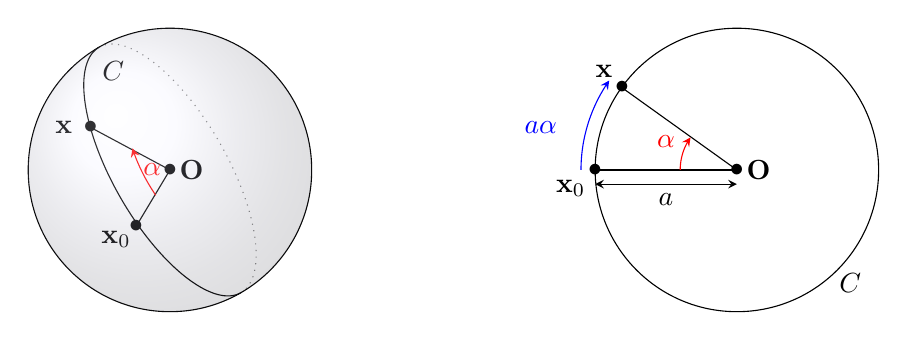
\begin{tikzpicture}[scale=1.8]
	% \draw [color=gray] (-1.5,-1.5) grid[step=0.1] (1.5,1.5); 
	\draw [rotate=-60,samples=100,domain=0:-180] plot({cos(\x)},{0.4*sin(\x)});
	\draw [rotate=-60,samples=100,domain=0:-180,color=gray,dotted] plot({cos(\x)},{-0.4*sin(\x)});
	\draw (-0.4,0.7) node {$C$} ; 
	\draw (-0.24,-0.4) node {$\bullet$} ;
	\draw (-0.38,-0.49) node {$\mathbf{x}_0$} ;
	\draw (0,0) node {$\bullet$} ;
	\draw (0,0) node[right] {$\mathbf{O}$} ;
	\draw (0,0) -- (-0.56,0.3) ;
	\draw (0,0) -- (-0.24,-0.4) ;
	\draw (-0.56,0.3) node {$\bullet$} ;
	\draw (-0.75,0.3) node {$\mathbf{x}$} ;
	\draw [rotate=-60,>=stealth, ->,color=red,domain=-78:-122] plot({0.5*cos(\x)},{0.18*sin(\x)});
	\draw [color=red] (-0.125,0) node {$\alpha$} ;
    \draw (0,0) circle (1cm);
    \shade[ball color=blue!10!white,opacity=0.20] (0,0) circle (1cm);

    \draw (4,0) circle (1cm);
    \draw (4,0) node {$\bullet$};
    \draw (4,0) node[right] {$\mathbf{O}$};
    \draw (3,0) node {$\bullet$};
    \draw (3,0) node[below left] {$\mathbf{x}_0$};
    \draw (4-.81,.58) node {$\bullet$};
    \draw (4-.81,.58) node[above left] {$\mathbf{x}$};
    \draw (3,0) -- (4,0);
    \draw (4-.81,.58) -- (4,0);
    \draw [>=stealth, <-,color=red,domain=145:180] plot({4+.4*cos(\x)},{.4*sin(\x)});
    \draw (3.5,.2) node[color=red] {$\alpha$};
    \draw [>=stealth, <-,color=blue,domain=145:180] plot({4+1.1*cos(\x)},{1.1*sin(\x)});
    \draw (2.8,.3) node[left, color=blue] {$a \alpha$};
    \draw [>=stealth, <->] (3,-.1) -- (4,-.1);
    \draw (3.5,-.1) node[below] {$a$}; 
    \draw (4.8,-.8) node {$C$};
\end{tikzpicture}
\end{center}
\caption{Un grand cercle sur la sphère $\mathbb{S}_a^2$. L'angle $\alpha$ est tel que $\widehat{\mathbf{x}_0 \mathbf{x}} = \alpha$ et l'abscisse curviligne de $\mathbf{x}$ comptée à partir de $\mathbf{x}_0$ est $a \alpha$.}
\label{fig: grand cercle}
\end{figure}

Soit $\overline{\mathbf{x}} \in \mathbb{S}_a^2$ fixé. Soient $C_1$ et $C_2$ deux grands cercles distincts arbitraires tels que $\overline{\mathbf{x}} \in C_1 \cap C_2$.
Soient $\alpha$ et $\beta$ les abscisses curvilignes le long de $C_1$ et $C_2$, définies à partir de $\mathbf{x}_{1,0} \in C_1$ et $\mathbf{x}_{2,0} \in C_2$ arbitrairement choisis. On définit les vecteurs $\mathbf{e}_{\alpha}(\overline{\mathbf{x}})$ et $\mathbf{e}_{\beta}(\overline{\mathbf{x}})$ (Fig. \ref{fig: e_alpha et e_beta}) par

\begin{equation}
\mathbf{e}_{\alpha}(\overline{\mathbf{x}}) = \dfrac{d \mathbf{x}}{d \alpha}(\overline{\mathbf{x}}) \text{ et } \mathbf{e}_{\beta}(\overline{\mathbf{x}}) = \dfrac{d \mathbf{x}}{d \beta}(\overline{\mathbf{x}}).
\end{equation}
Les vecteurs $\mathbf{e}_{\alpha}(\overline{\mathbf{x}})$ et $\mathbf{e}_{\beta}(\overline{\mathbf{x}})$ sont tangents aux cercles $C_1$ et $C_2$. On note $\alpha \mapsto \mathbf{x}(\alpha)$ (resp.  $\beta \mapsto \mathbf{x}(\beta)$) le paramétrage du cercle $C_1$ (resp. $C_2$) par l'angle $\alpha$ (resp. $\beta$).

\begin{figure}[htbp]
\begin{center}
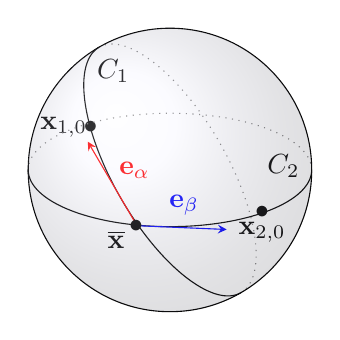
\begin{tikzpicture}[scale=1.8]
	\draw [rotate=-60,samples=100,domain=0:-180] plot({cos(\x)},{0.4*sin(\x)});
	\draw [rotate=-60,samples=100,domain=0:-180,color=gray,dotted] plot({cos(\x)},{-0.4*sin(\x)});
	\draw (-.56,.3) node {$\bullet$} ;
	\draw (-0.75,0.3) node {$\mathbf{x}_{1,0}$} ;
	\draw (-0.4,0.7) node {$C_1$} ; 
	
	\draw [samples=100,domain=0:-180] plot({cos(\x)},{0.4*sin(\x)});
	\draw [samples=100,domain=0:-180,color=gray,dotted] plot({cos(\x)},{-0.4*sin(\x)});
	\draw (0.65,-0.3) node {$\bullet$} ;
	\draw (0.65,-0.3) node[below] {$\mathbf{x}_{2,0}$} ;
	\draw (0.8,0.03) node {$C_2$} ;
	
	\draw [>=stealth, ->, color=blue] (-0.24,-0.393) -- (0.4,-0.42) ;
	\draw [color=blue] (0.1,-0.25) node {$\mathbf{e}_{\beta}$} ;	
	\draw [>=stealth, ->, color=red] (-0.24,-0.38) -- (-0.58,0.20) ;	
	\draw [color=red] (-0.25,0) node {$\mathbf{e}_{\alpha}$} ;
	
	\draw (-0.24,-0.4) node {$\bullet$} ;
	\draw (-0.38,-0.49) node {$\overline{\mathbf{x}}$} ;
	\draw (0,0) circle (1cm);
    \shade[ball color=blue!10!white,opacity=0.20] (0,0) circle (1cm);
\end{tikzpicture}
\end{center}
\caption{Vecteurs $\mathbf{e}_{\alpha}$ et $\mathbf{e}_{\beta}$ associés au cercles $C_1$ et $C_2$ de $\mathbb{S}_a^2$.}
\label{fig: e_alpha et e_beta}
\end{figure}



En tout point $\mathbf{x} \in \mathbb{S}_a^2$, le \textit{plan tangent} $\mathbb{T}_{\mathbf{x}} \mathbb{S}_a^2$ est défini par :

\begin{definition}
On appelle \textit{plan tangent} à la sphère $\mathbb{S}_a^2$ au point $\overline{\mathbf{x}}$ le plan :
\begin{equation}
\mathbb{T}_{\overline{\mathbf{x}}} \mathbb{S}_a^2 = \left\lbrace \mathbf{m} \in \mathbb{R}^3 \ \overrightarrow{\overline{\mathbf{x}} \mathbf{m}} \perp \overrightarrow{O\mathbf{\overline{x}}} \right\rbrace.
\end{equation}
\end{definition}

\begin{proposition}
Soit $\overline{\mathbf{x}} \in \mathbb{S}_a^2$, alors :
\begin{equation}
\mathbf{e}_{\alpha}(\overline{\mathbf{x}})\text{, } \mathbf{e}_{\beta}(\overline{\mathbf{x}}) \in \mathbb{T}_{\overline{\mathbf{x}}} \mathbb{S}_a^2.
\end{equation}
\end{proposition}


\begin{proof}
Soit $\mathbf{x}$ est un point quelconque de $\mathbb{S}_a^2$. Nous adoptons la notation $\| \mathbf{x} \|= \| \mathbf{Ox} \|$. On a $\| \mathbf{x} \|^2 = \mathbf{x} \cdot \mathbf{x} = a^2$ constant. Alors en dérivant par rapport à $\alpha$, on a :
 
\begin{equation*}
\begin{array}{rcl}
0 & = & \dfrac{d}{d \alpha} ( a^2 )\\
  & = & \dfrac{d}{d \alpha} ( \mathbf{x} \cdot \mathbf{x} )\\
  & = & 2 \mathbf{x} \cdot \dfrac{d \mathbf{x}}{d \alpha}.
\end{array}
\end{equation*}
En particulier, en $\overline{\mathbf{x}}$, on a :
\begin{equation}
\overline{\mathbf{x}} \cdot \mathbf{e}_{\alpha}(\overline{\mathbf{x}}) = 0
\end{equation}
donc $\mathbf{e}_{\alpha}(\overline{\mathbf{x}}) \in \mathbb{T}_{\overline{\mathbf{x}}} \mathbb{S}_a^2$. En dérivant par rapport à $\beta$, on a $\mathbf{e}_{\beta}(\overline{\mathbf{x}}) \in \mathbb{T}_{\overline{\mathbf{x}}} \mathbb{S}_a^2$.
\end{proof}

Les vecteurs $\mathbf{e}_{\alpha}(\overline{\mathbf{x}})$ et $\mathbf{e}_{\beta}(\overline{\mathbf{x}})$ sont dans le plan $\mathbb{T}_{\overline{\mathbf{x}}}\mathbb{S}_a^2$. De plus, $C_1 \neq C_2$ donc $\mathbf{e}_{\alpha}(\overline{\mathbf{x}})$ et $\mathbf{e}_{\beta}(\overline{\mathbf{x}})$ ne sont pas colinéaires. On en déduit que $\mathbf{e}_{\alpha}(\overline{\mathbf{x}})$ et $\mathbf{e}_{\beta}(\overline{\mathbf{x}})$ engendrent $\mathbb{T}_{\overline{\mathbf{x}}} \mathbb{S}_a^2$. En général, $\mathbf{e}_{\alpha}(\overline{\mathbf{x}})$ et $\mathbf{e}_{\beta}(\overline{\mathbf{x}})$ ne sont pas orthogonaux.

\begin{definition}
On définit $(\mathbf{e}^{\alpha}(\overline{\mathbf{x}}), \mathbf{e}^{\beta}(\overline{\mathbf{x}}))$ la \textit{base duale} de $(\mathbf{e}_{\alpha}(\overline{\mathbf{x}}), \mathbf{e}_{\beta}(\overline{\mathbf{x}}))$.
Les vecteurs $\mathbf{e}^{\alpha}(\overline{\mathbf{x}})$ et $\mathbf{e}^{\beta}(\overline{\mathbf{x}})$ sont les vecteurs de $\mathbb{T}_{\overline{\mathbf{x}}}\mathbb{S}_a^2$ vérifiant :

\begin{equation}
\left\lbrace
\begin{array}{rcccl}
\mathbf{e}_{\alpha}(\overline{\mathbf{x}}) \cdot \mathbf{e}^{\alpha}(\overline{\mathbf{x}}) & = & 1 & = & \mathbf{e}_{\beta}(\overline{\mathbf{x}}) \cdot \mathbf{e}^{\beta}(\overline{\mathbf{x}}) \\
\mathbf{e}_{\alpha}(\overline{\mathbf{x}}) \cdot \mathbf{e}^{\beta}(\overline{\mathbf{x}}) & = & 0 & = & \mathbf{e}_{\beta}(\overline{\mathbf{x}}) \cdot \mathbf{e}^{\alpha}(\overline{\mathbf{x}}).
\end{array}
\right.
\label{eq: dualite alpha beta}
\end{equation}
\end{definition}

\begin{proposition}
La base $(\mathbf{e}^{\alpha}(\overline{\mathbf{x}}), \mathbf{e}^{\beta}(\overline{\mathbf{x}}))$, duale de $(\mathbf{e}_{\alpha}(\overline{\mathbf{x}}), \mathbf{e}_{\beta}(\overline{\mathbf{x}}))$ est définie de façon unique.
\end{proposition}

\begin{proof}
Il suffit de remarquer que
\begin{equation}
\begin{bmatrix}
\mathbf{e}_{\alpha}(\overline{\mathbf{x}}) , \mathbf{e}_{\beta}(\overline{\mathbf{x}})
\end{bmatrix}^T \cdot 
\begin{bmatrix}
\mathbf{e}^{\alpha}(\overline{\mathbf{x}}) , \mathbf{e}^{\beta}(\overline{\mathbf{x}})
\end{bmatrix} = \Id.
\end{equation}
Alors 
\begin{equation}
\begin{bmatrix}
\mathbf{e}^{\alpha}(\overline{\mathbf{x}}) , \mathbf{e}^{\beta}(\overline{\mathbf{x}})
\end{bmatrix} = 
\begin{bmatrix}
\mathbf{e}_{\alpha}(\overline{\mathbf{x}}) , \mathbf{e}_{\beta}(\overline{\mathbf{x}})
\end{bmatrix}^{-T}.
\end{equation}
\end{proof}

A partir de ces différentes bases, le \textit{gradient} est donné par la définition suivante.

\begin{definition}
Soit $h : \mathbb{S}_a^2 \rightarrow \mathbb{R}$ une fonction régulière. Le gradient de $h$, $\nabla_T h(\mathbf{x}) \in \mathbb{T}_{\mathbf{x}}\mathbb{S}^2_a$, est défini par
\begin{equation}
\nabla_{T} h(\overline{\mathbf{x}}) = \dfrac{\partial}{\partial \alpha} \left( h(\overline{\mathbf{x}}) \right)_{| \mathbf{x} \in C_1} \mathbf{e}^{\alpha}(\overline{\mathbf{x}}) + \dfrac{\partial}{\partial \beta}\left(  h(\overline{\mathbf{x}}) \right)_{| \mathbf{x} \in C_2} \mathbf{e}^{\beta}(\overline{\mathbf{x}}).
\label{eq: gradient}
\end{equation}
\end{definition}
Pour alléger les notations, nous noterons abusivement les quantités $h$, $\mathbf{e}_{\alpha}$, $\mathbf{e}^{\beta}$ etc. au lieu de $h(\bar{\mathbf{x}})$, $\mathbf{e}_{\alpha}(\bar{\mathbf{x}})$, $\mathbf{e}^{\beta}(\bar{\mathbf{x}})$, etc.


\begin{proposition}
Soit $u: \mathbb{R}^3 \mapsto \mathbb{R}$ et $\mathbf{x} \in \mathbb{R}^3$. On pose $\hat{u} : = u_{|\mathbb{S}_a^2}$ la restriction de $u$ à la sphère $\mathbb{S}_a^2$. Alors $\nabla_{T} \hat{u} (\mathbf{x})$ est la projection orthogonale de $\nabla_{\mathbb{R}^3} u (\mathbf{x})$ sur le plan tangent $\mathbb{T}_{\mathbf{x}} \mathbb{S}_a^2$ :

\begin{equation}
\nabla_T \hat{u} = \nabla_{\mathbb{R}^3} u - \mathbf{n} \left( \mathbf{n} \cdot \nabla_{\mathbb{R}^3} u \right)
\end{equation}

avec $\mathbf{n}$ la normale unitaire extérieure.
\label{prop:gradient_project}
\end{proposition}

\begin{proof}
On montre que les deux termes sont égaux dans trois directions distinctes. On pose $\mathbf{n}$ la normale unitaire extérieure à la sphère $\mathbb{S}_a^2$.
\begin{itemize}
\item Direction $\mathbf{e}_{\alpha}$ :
d'une part on a :
\begin{equation}
\nabla_T \hat{u} \cdot \mathbf{e}_{\alpha} = \dfrac{\partial \hat{u}}{\partial \alpha}_{| \mathbf{x} \in C_1}= \dfrac{\partial u}{\partial \alpha}_{| \mathbf{x} \in C_1}.
\end{equation}
D'autre part, on a :
\begin{equation}
\left( \nabla_{\mathbb{R}^3} u - \mathbf{n} \left( \mathbf{n} \cdot \nabla_{\mathbb{R}^3} u \right) \right) \cdot \mathbf{e}_{\alpha} = \nabla_{\mathbb{R}^3} u \cdot \mathbf{e}_{\alpha}
\end{equation}
car $\mathbf{n}$ est normal à la sphère donc $\mathbf{n}$ est normal à $\mathbf{e}_{\alpha}$.
Or :
\begin{equation}
\nabla_{\mathbb{R}^3} u \cdot \mathbf{e}_{\alpha} = \dfrac{\partial u}{\partial \alpha}_{| \mathbf{x} \in C_1} = \nabla_T \hat{u} \cdot \mathbf{e}_{\alpha}.
\end{equation}

\item Dans la direction $\mathbf{e}_{\beta}$, on a de la même manière :
\begin{equation}
\nabla_{\mathbb{R}^3} u \cdot \mathbf{e}_{\beta} = \nabla_T \hat{u} \cdot \mathbf{e}_{\beta}.
\end{equation}

\item Dans la direction $\mathbf{n}$ on a d'une part :
\begin{equation}
\nabla_T \hat{u} \cdot \mathbf{n} = 0 
\end{equation}
car $\nabla_T \hat{u}$ est tangent à la sphère. D'autre part :
\begin{equation}
\left( \nabla_{\mathbb{R}^3} u - \mathbf{n} \left( \mathbf{n} \cdot \nabla_{\mathbb{R}^3} u \right) \right) \cdot \mathbf{n} = \nabla_{\mathbb{R}^3} u \cdot \mathbf{n}- \mathbf{n} \cdot \nabla_{\mathbb{R}^3} u = 0.
\end{equation}
\end{itemize}
Or, $(\mathbf{e}_{\alpha}, \mathbf{e}_{\beta}, \mathbf{n})$ est une base de $\mathbb{R}^3$, d'où l'égalité souhaitée.
\end{proof}




















\subsection{Définition de la Cubed-Sphere}

Dans cette partie, on définit la Grille Cubed-Sphere associée à la base orthonormée $(\mathbf{i}, \mathbf{j}, \mathbf{k})$ de $\mathbb{R}^3$.
On définit les points suivants (Voir Figure \ref{fig: sphere NSEWFB}) sur la sphère $\mathbb{S}_a^2$ :
\begin{itemize}
\item $\mathbf{N}$ le point de coordonnées dans $\mathbb{R}^3$ : $(0,0,a)$,
\item $\mathbf{S}$ le point de coordonnées $(0,0,-a)$,
\item $\mathbf{E}$ le point de coordonnées $(0,a,0)$,
\item $\mathbf{W}$ le point de coordonnées $(0,-a,0)$,
\item $\mathbf{F}$ le point de coordonnées $(a,0,0)$,
\item $\mathbf{B}$ le point de coordonnées $(-a,0,0)$.
\end{itemize}


\begin{figure}[htbp]
\begin{center}
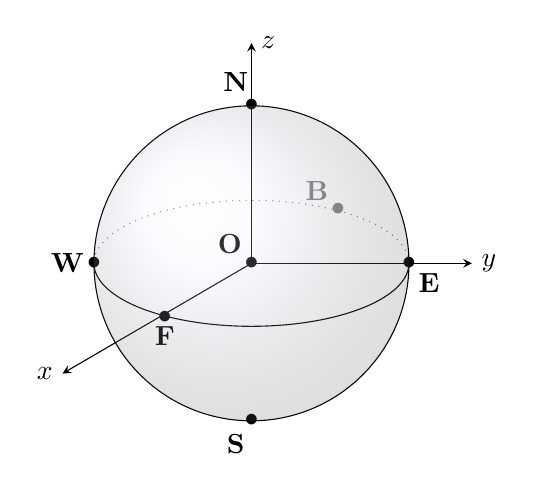
\begin{tikzpicture}[scale=2]
	\draw [samples=100,domain=-180:0] plot({cos(\x)},{0.4*sin(\x)});
	\draw [dotted, color=black!50, samples=100,domain=0:180] plot({cos(\x)},{0.4*sin(\x)});

	\draw  (0,0) node {$\bullet$} ;
	\draw  (0,0) node[above left] {$\mathbf{O}$} ;
	\draw  (0,1) node {$\bullet$} ;
	\draw  (-0.1,1.15) node {$\mathbf{N}$} ;
	\draw  (0,-1) node {$\bullet$} ;
	\draw  (-0.1,-1.15) node {$\mathbf{S}$} ;
	\draw  (1,0) node {$\bullet$} ;
	\draw  (1,0) node[below right] {$\mathbf{E}$} ;
	\draw  (-1,0) node {$\bullet$} ;
	\draw  (-1,0) node[left] {$\mathbf{W}$} ;	
	\draw  (-0.55,-0.34) node {$\bullet$} ;
	\draw  (-0.55,-0.34) node[below] {$\mathbf{F}$} ;	
	\draw  (0.55,0.34) node[color=black!50] {$\bullet$} ;
	\draw  (0.55,0.34) node[color=black!50, above left] {$\mathbf{B}$} ;	
	
	\draw [>=stealth, ->] (0,0) -- (-1.2,-0.7) ;
	\draw  (-1.2,-0.7) node[left] {$x$} ;
	\draw [>=stealth, ->] (0,0) -- (0,1.4) ;
	\draw  (0,1.4) node[right] {$z$} ;
	\draw [>=stealth, ->] (0,0) -- (1.4,0) ;
	\draw  (1.4,0) node[right] {$y$} ;
	\draw (0,0) circle (1cm);
    \shade[ball color=blue!10!white,opacity=0.20] (0,0) circle (1cm);
\end{tikzpicture}
\end{center}
\caption{Sphère $\mathbb{S}_a^2$ avec les 6 points $\mathbf{N}$ (Nord), $\mathbf{S}$ (Sud), $\mathbf{E}$ (Est), $\mathbf{W}$ (Ouest), $\mathbf{F}$ (Avant) et $\mathbf{B}$ (Arrière).}
\label{fig: sphere NSEWFB}
\end{figure}

Un grand cercle est l'intersection de la sphère $\mathbb{S}_a^2$ avec un plan contenant le point $\mathbf{O}$. On définit les grands cercles suivants (Fig. \ref{fig:grandscerclespanelI}) :

\begin{itemize}
\item $C_V^1 = \Vect(\mathbf{i}-\mathbf{j}, \mathbf{k}) \cap \mathbb{S}_a^2$,
\item $C_V^2 = \Vect(\mathbf{i}+\mathbf{j}, \mathbf{k}) \cap \mathbb{S}_a^2$, il s'agit d'une rotation de $C_V^1$ d'un angle de $\pi/2$ autour de $(Oz)$,
\item $C_{II}^1 = \Vect(\mathbf{i}+\mathbf{k}, \mathbf{j}) \cap \mathbb{S}_a^2$,
\item $C_{II}^2 = \Vect(\mathbf{i}-\mathbf{k}, \mathbf{j}) \cap \mathbb{S}_a^2$, le cercle $C_{II}^2$ est une rotation de $C_{II}^1$ d'un angle de $\pi/2$ autour de $(Oy)$,
\item $C_I^1=\Vect(\mathbf{j}-\mathbf{k},\mathbf{i}) \cap \mathbb{S}_a^2$,
\item $C_I^2=\Vect(\mathbf{j}+\mathbf{k},\mathbf{i}) \cap \mathbb{S}_a^2$, $C_I^2$ est une rotation de $C_I^1$ autour de $(Ox)$ d'un angle de $\pi/2$.
\end{itemize}

\begin{figure}[htbp]
\begin{center}
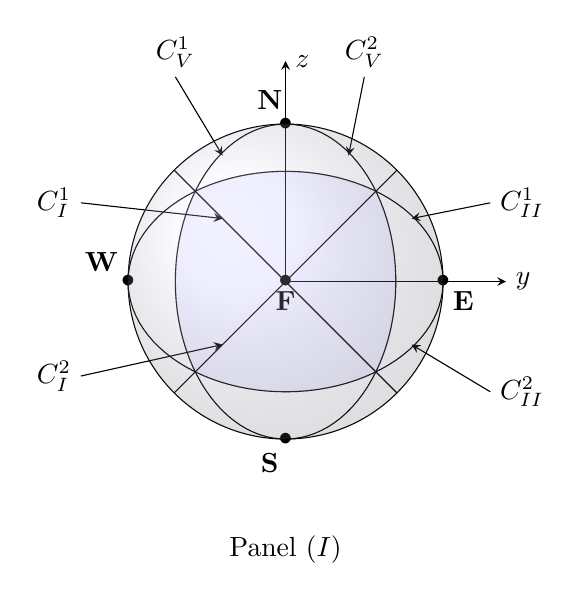
\begin{tikzpicture}[scale=2]
	%\draw [color=gray] (-1.5,-1.5) grid[step=0.1] (1.5,1.5);
	\draw [samples=100,domain=-180:180] plot({cos(\x)},{0.7*sin(\x)});
	\draw [samples=100,domain=180:-180] plot({0.7*cos(\x)},{sin(\x)}); 
	
	\filldraw[draw=black,fill=blue!30!white,opacity=0.20]
	plot [smooth,domain=-35:35] ({0.7*cos(\x)},{sin(\x)})
	-- plot [smooth,domain=55:125] ({cos(\x)},{0.7*sin(\x)})
	-- plot [smooth,domain=140:215] ({0.7*cos(\x)},{sin(\x)})
	-- plot [smooth,domain=230:305] ({cos(\x)},{0.7*sin(\x)})
	-- cycle;
	
	\draw (-0.707,0.707) -- (0.707,-0.707) ;
	\draw [>=stealth, <-] (-0.4,0.4) -- (-1.3,0.5) ;
	\draw  (-1.3,0.5) node[left] {$C_I^1$} ;
	\draw (-0.707,-0.707) -- (0.707,0.707) ;
	\draw [>=stealth, <-] (-0.4,-0.4) -- (-1.3,-0.6) ;
	\draw  (-1.3,-0.6) node[left] {$C_I^2$} ;
	
	\draw [>=stealth, ->] (0.5,1.3) -- (0.4,0.8) ;
	\draw  (0.5,1.3) node[above] {$C_V^2$} ;
	\draw [>=stealth, ->] (-0.7,1.3) -- (-0.4,0.8) ;
	\draw  (-0.7,1.3) node[above] {$C_V^1$} ;
	\draw [>=stealth, ->] (1.3,0.5) -- (0.8,0.4) ;
	\draw  (1.3,0.5) node[right] {$C_{II}^1$} ;
	\draw [>=stealth, ->] (1.3,-0.7) -- (0.8,-0.4) ;
	\draw  (1.3,-0.7) node[right] {$C_{II}^2$} ;
	
	\draw [>=stealth, ->] (0,0) -- (0,1.4) ;
	\draw  (0,1.4) node[right] {$z$} ;
	\draw [>=stealth, ->] (0,0) -- (1.4,0) ;
	\draw  (1.4,0) node[right] {$y$} ;
	
	\draw  (0,1) node {$\bullet$} ;
	\draw  (-0.1,1.15) node {$\mathbf{N}$} ;
	\draw  (0,-1) node {$\bullet$} ;
	\draw  (-0.1,-1.15) node {$\mathbf{S}$} ;
	\draw  (1,0) node {$\bullet$} ;
	\draw  (1,0) node[below right] {$\mathbf{E}$} ;
	\draw  (-1,0) node {$\bullet$} ;
	\draw  (-1,0) node[above left] {$\mathbf{W}$} ;
	\draw  (0,0) node {$\bullet$} ;
	\draw  (0,0) node[below] {$\mathbf{F}$} ;
	
	\draw  (0,-1.7) node {Panel $(I)$} ;

	\draw (0,0) circle (1cm);
    \shade[ball color=blue!10!white,opacity=0.20] (0,0) circle (1cm);

\end{tikzpicture}
\caption{\label{fig:grandscerclespanelI} Les 6 grands cercles $C_I^1$, $C_I^2$, $C_{II}^1$, $C_{II}^2$, $C_V^1$ et $C_V^1$ vus depuis le panel $(I)$.}
\end{center}
\end{figure}

La construction de la Cubed-Sphere fait intervenir six zones recouvrant la sphère $\mathbb{S}_a^2$ appelées \textit{panels}. Chaque panel est délimité par quatre grands cercles (Fig. \ref{fig: panel I to VI}).

\begin{definition}
\begin{itemize}
\item  \textbf{Panels $\mathbf{(I)}$ et $\mathbf{(III)}$ : }Les panels $(I)$ et $(III)$ sont définis par les points de $\mathbb{S}_a^2$ délimités par les grands cercles $C_V^1$, $C_V^2$, $C_{II}^1$ et $C_{II}^2$. Le panel $(III)$ est le symétrique du panel $(I)$ par la symétrie ponctuelle de centre $\mathbf{O}$. Le panel $(I)$ ne contient que des points $(x,y,z)$ tels que $x>0$, le panel $(III)$ ne contient que des points tels que $x<0$.
\item \textbf{Panels $\mathbf{(II)}$ et $\mathbf{(IV)}$ : }Les panels $(II)$ et $(IV)$ sont définis par les points de $\mathbb{S}_a^2$ délimités par les grands cercles $C_V^1$, $C_V^2$, $C_{I}^1$ et $C_{I}^2$. Le panel $(IV)$ est le symétrique du panel $(II)$ par la symétrie ponctuelle de centre $\mathbf{O}$. Le panel $(II)$ ne contient que des points $(x,y,z)$ tels que $y>0$, le panel $(IV)$ ne contient que des points tels que $y<0$.
\item \textbf{Panels $\mathbf{(V)}$ et $\mathbf{(VI)}$ : }Les panels $(V)$ et $(VI)$ sont définis par les points de $\mathbb{S}_a^2$ délimités par les grands cercles $C_I^1$, $C_I^2$, $C_{II}^1$ et $C_{II}^2$. Le panel $(VI)$ est le symétrique du panel $(V)$ par la symétrie ponctuelle de centre $\mathbf{O}$. Le panel $(V)$ ne contient que des points $(x,y,z)$ tels que $z>0$, le panel $(VI)$ ne contient que des points tels que $z<0$.
\end{itemize}
\end{definition}






\begin{figure}[htbp]
\begin{center}
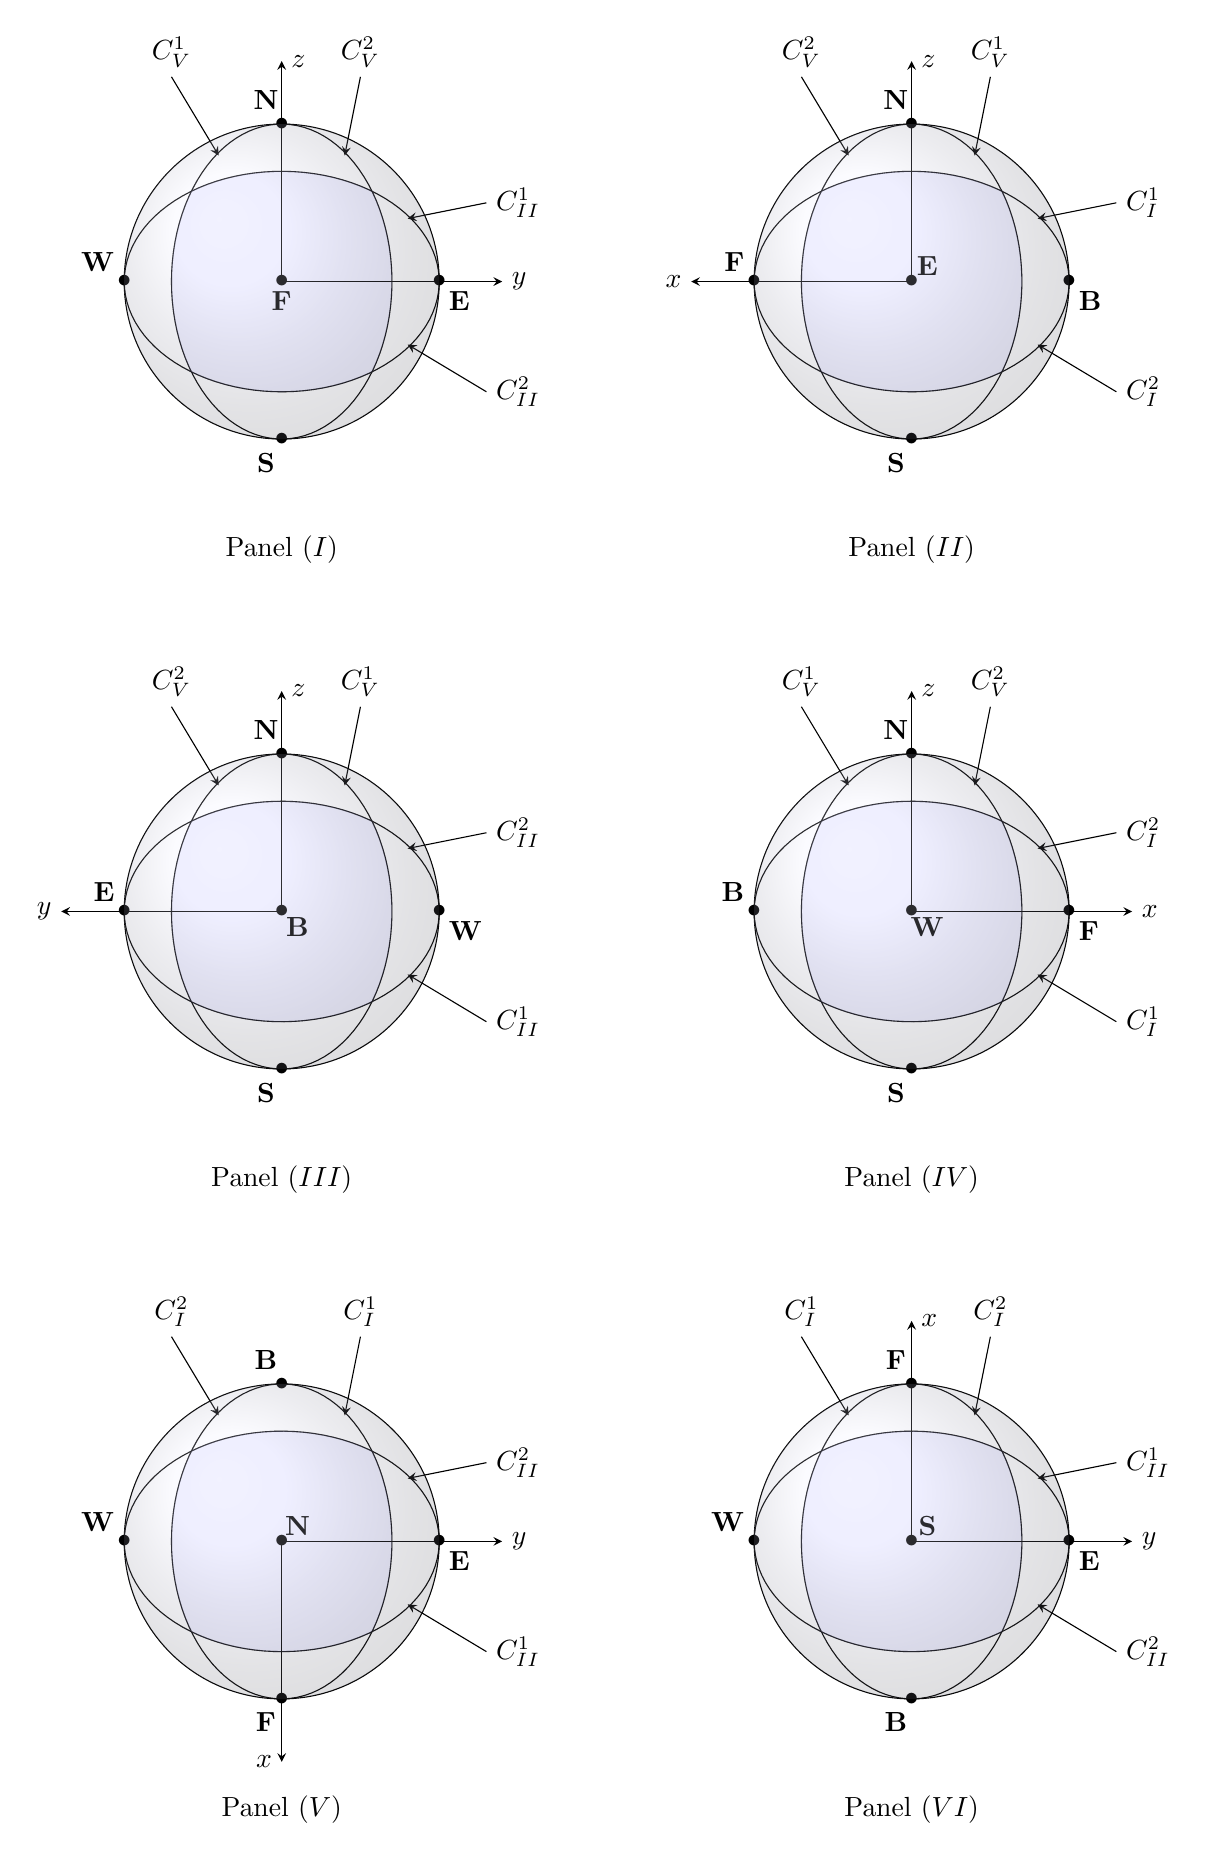
\begin{tikzpicture}[scale=2]
	%\draw [color=gray] (-1.5,-1.5) grid[step=0.1] (1.5,1.5);
	\draw [samples=100,domain=-180:180] plot({cos(\x)},{0.7*sin(\x)});
	\draw [samples=100,domain=180:-180] plot({0.7*cos(\x)},{sin(\x)}); 
	
	\filldraw[draw=black,fill=blue!30!white,opacity=0.20]
	plot [smooth,domain=-35:35] ({0.7*cos(\x)},{sin(\x)})
	-- plot [smooth,domain=55:125] ({cos(\x)},{0.7*sin(\x)})
	-- plot [smooth,domain=140:215] ({0.7*cos(\x)},{sin(\x)})
	-- plot [smooth,domain=230:305] ({cos(\x)},{0.7*sin(\x)})
	-- cycle;
	
	\draw [>=stealth, ->] (0.5,1.3) -- (0.4,0.8) ;
	\draw  (0.5,1.3) node[above] {$C_V^2$} ;
	\draw [>=stealth, ->] (-0.7,1.3) -- (-0.4,0.8) ;
	\draw  (-0.7,1.3) node[above] {$C_V^1$} ;
	\draw [>=stealth, ->] (1.3,0.5) -- (0.8,0.4) ;
	\draw  (1.3,0.5) node[right] {$C_{II}^1$} ;
	\draw [>=stealth, ->] (1.3,-0.7) -- (0.8,-0.4) ;
	\draw  (1.3,-0.7) node[right] {$C_{II}^2$} ;
	
	\draw [>=stealth, ->] (0,0) -- (0,1.4) ;
	\draw  (0,1.4) node[right] {$z$} ;
	\draw [>=stealth, ->] (0,0) -- (1.4,0) ;
	\draw  (1.4,0) node[right] {$y$} ;
	
	\draw  (0,1) node {$\bullet$} ;
	\draw  (-0.1,1.15) node {$\mathbf{N}$} ;
	\draw  (0,-1) node {$\bullet$} ;
	\draw  (-0.1,-1.15) node {$\mathbf{S}$} ;
	\draw  (1,0) node {$\bullet$} ;
	\draw  (1,0) node[below right] {$\mathbf{E}$} ;
	\draw  (-1,0) node {$\bullet$} ;
	\draw  (-1,0) node[above left] {$\mathbf{W}$} ;
	\draw  (0,0) node {$\bullet$} ;
	\draw  (0,0) node[below] {$\mathbf{F}$} ;
	
	\draw  (0,-1.7) node {Panel $(I)$} ;

	\draw (0,0) circle (1cm);
    \shade[ball color=blue!10!white,opacity=0.20] (0,0) circle (1cm);




	\draw [samples=100,domain=-180:180] plot({4+cos(\x)},{0.7*sin(\x)});
	\draw [samples=100,domain=180:-180] plot({4+0.7*cos(\x)},{sin(\x)}); 
	
	\filldraw[draw=black,fill=blue!30!white,opacity=0.20]
	plot [smooth,domain=-35:35] ({4+0.7*cos(\x)},{sin(\x)})
	-- plot [smooth,domain=55:125] ({4+cos(\x)},{0.7*sin(\x)})
	-- plot [smooth,domain=140:215] ({4+0.7*cos(\x)},{sin(\x)})
	-- plot [smooth,domain=230:305] ({4+cos(\x)},{0.7*sin(\x)})
	-- cycle;
	
	\draw [>=stealth, ->] (4.5,1.3) -- (4.4,0.8) ;
	\draw  (4.5,1.3) node[above] {$C_V^1$} ;
	\draw [>=stealth, ->] (3.3,1.3) -- (3.6,0.8) ;
	\draw  (3.3,1.3) node[above] {$C_V^2$} ;
	\draw [>=stealth, ->] (5.3,0.5) -- (4.8,0.4) ;
	\draw  (5.3,0.5) node[right] {$C_{I}^1$} ;
	\draw [>=stealth, ->] (5.3,-0.7) -- (4.8,-0.4) ;
	\draw  (5.3,-0.7) node[right] {$C_{I}^2$} ;
	
	\draw [>=stealth, ->] (4,0) -- (4,1.4) ;
	\draw  (4,1.4) node[right] {$z$} ;
	\draw [>=stealth, ->] (4,0) -- (4-1.4,0) ;
	\draw  (4-1.4,0) node[left] {$x$} ;
	
	\draw  (4,1) node {$\bullet$} ;
	\draw  (4-0.1,1.15) node {$\mathbf{N}$} ;
	\draw  (4,-1) node {$\bullet$} ;
	\draw  (4-0.1,-1.15) node {$\mathbf{S}$} ;
	\draw  (5,0) node {$\bullet$} ;
	\draw  (5,0) node[below right] {$\mathbf{B}$} ;
	\draw  (4-1,0) node {$\bullet$} ;
	\draw  (4-1,0) node[above left] {$\mathbf{F}$} ;
	\draw  (4,0) node {$\bullet$} ;
	\draw  (4.1,0.1) node {$\mathbf{E}$} ;
	
	\draw  (4,-1.7) node {Panel $(II)$} ;

	\draw (4,0) circle (1cm);
    \shade[ball color=blue!10!white,opacity=0.20] (4,0) circle (1cm);






	\draw [samples=100,domain=-180:180] plot({cos(\x)},{-4+0.7*sin(\x)});
	\draw [samples=100,domain=180:-180] plot({0.7*cos(\x)},{-4+sin(\x)}); 
	
	\filldraw[draw=black,fill=blue!30!white,opacity=0.20]
	plot [smooth,domain=-35:35] ({0.7*cos(\x)},{-4+sin(\x)})
	-- plot [smooth,domain=55:125] ({cos(\x)},{-4+0.7*sin(\x)})
	-- plot [smooth,domain=140:215] ({0.7*cos(\x)},{-4+sin(\x)})
	-- plot [smooth,domain=230:305] ({cos(\x)},{-4+0.7*sin(\x)})
	-- cycle;
	
	\draw [>=stealth, ->] (0.5,-4+1.3) -- (0.4,-4+0.8) ;
	\draw  (0.5,-4+1.3) node[above] {$C_V^1$} ;
	\draw [>=stealth, ->] (-0.7,-4+1.3) -- (-0.4,-4+0.8) ;
	\draw  (-0.7,-4+1.3) node[above] {$C_V^2$} ;
	\draw [>=stealth, ->] (1.3,-4+0.5) -- (0.8,-4+0.4) ;
	\draw  (1.3,-4+0.5) node[right] {$C_{II}^2$} ;
	\draw [>=stealth, ->] (1.3,-4-0.7) -- (0.8,-4-0.4) ;
	\draw  (1.3,-4-0.7) node[right] {$C_{II}^1$} ;
	
	\draw [>=stealth, ->] (0,-4) -- (0,-4+1.4) ;
	\draw  (0,-4+1.4) node[right] {$z$} ;
	\draw [>=stealth, ->] (0,-4) -- (-1.4,-4) ;
	\draw  (-1.4,-4) node[left] {$y$} ;
	
	\draw  (0,-4+1) node {$\bullet$} ;
	\draw  (-0.1,-4+1.15) node {$\mathbf{N}$} ;
	\draw  (0,-4-1) node {$\bullet$} ;
	\draw  (-0.1,-4-1.15) node {$\mathbf{S}$} ;
	\draw  (1,-4) node {$\bullet$} ;
	\draw  (1,-4) node[below right] {$\mathbf{W}$} ;
	\draw  (-1,-4) node {$\bullet$} ;
	\draw  (-1,-4) node[above left] {$\mathbf{E}$} ;
	\draw  (0,-4) node {$\bullet$} ;
	\draw  (0.1,-4.1) node {$\mathbf{B}$} ;
	
	\draw  (0,-4-1.7) node {Panel $(III)$} ;

	\draw (0,-4) circle (1cm);
    \shade[ball color=blue!10!white,opacity=0.20] (0,-4) circle (1cm);




	\draw [samples=100,domain=-180:180] plot({4+cos(\x)},{-4+0.7*sin(\x)});
	\draw [samples=100,domain=180:-180] plot({4+0.7*cos(\x)},{-4+sin(\x)}); 
	
	\filldraw[draw=black,fill=blue!30!white,opacity=0.20]
	plot [smooth,domain=-35:35] ({4+0.7*cos(\x)},{-4+sin(\x)})
	-- plot [smooth,domain=55:125] ({4+cos(\x)},{-4+0.7*sin(\x)})
	-- plot [smooth,domain=140:215] ({4+0.7*cos(\x)},{-4+sin(\x)})
	-- plot [smooth,domain=230:305] ({4+cos(\x)},{-4+0.7*sin(\x)})
	-- cycle;
	
	\draw [>=stealth, ->] (4+0.5,-4+1.3) -- (4+0.4,-4+0.8) ;
	\draw  (4+0.5,-4+1.3) node[above] {$C_V^2$} ;
	\draw [>=stealth, ->] (4-0.7,-4+1.3) -- (4-0.4,-4+.8) ;
	\draw  (4-0.7,-4+1.3) node[above] {$C_V^1$} ;
	\draw [>=stealth, ->] (4+1.3,-4+0.5) -- (4+0.8,-4+0.4) ;
	\draw  (4+1.3,-4+.5) node[right] {$C_{I}^2$} ;
	\draw [>=stealth, ->] (4+1.3,-4-0.7) -- (4+0.8,-4-0.4) ;
	\draw  (4+1.3,-4-0.7) node[right] {$C_{I}^1$} ;
	
	\draw [>=stealth, ->] (4,-4) -- (4,-4+1.4) ;
	\draw  (4,-4+1.4) node[right] {$z$} ;
	\draw [>=stealth, ->] (4,-4) -- (5.4,-4) ;
	\draw  (5.4,-4) node[right] {$x$} ;
	
	\draw  (4,-4+1) node {$\bullet$} ;
	\draw  (4-0.1,-4+1.15) node {$\mathbf{N}$} ;
	\draw  (4,-4-1) node {$\bullet$} ;
	\draw  (4-0.1,-4-1.15) node {$\mathbf{S}$} ;
	\draw  (5,-4) node {$\bullet$} ;
	\draw  (5,-4) node[below right] {$\mathbf{F}$} ;
	\draw  (4-1,-4) node {$\bullet$} ;
	\draw  (4-1,-4) node[above left] {$\mathbf{B}$} ;
	\draw  (4,-4) node {$\bullet$} ;
	\draw  (4.1,-4.1) node {$\mathbf{W}$} ;
	
	\draw  (4,-4-1.7) node {Panel $(IV)$} ;

	\draw (4,-4) circle (1cm);
    \shade[ball color=blue!10!white,opacity=0.20] (4,-4) circle (1cm);




	\draw [samples=100,domain=-180:180] plot({cos(\x)},{-8+0.7*sin(\x)});
	\draw [samples=100,domain=180:-180] plot({0.7*cos(\x)},{-8+sin(\x)}); 
	
	\filldraw[draw=black,fill=blue!30!white,opacity=0.20]
	plot [smooth,domain=-35:35] ({0.7*cos(\x)},{-8+sin(\x)})
	-- plot [smooth,domain=55:125] ({cos(\x)},{0.7*sin(\x)-8})
	-- plot [smooth,domain=140:215] ({0.7*cos(\x)},{sin(\x)-8})
	-- plot [smooth,domain=230:305] ({cos(\x)},{0.7*sin(\x)-8})
	-- cycle;
	
	\draw [>=stealth, ->] (0.5,1.3-8) -- (0.4,0.8-8) ;
	\draw  (0.5,1.3-8) node[above] {$C_I^1$} ;
	\draw [>=stealth, ->] (-0.7,1.3-8) -- (-0.4,0.8-8) ;
	\draw  (-0.7,1.3-8) node[above] {$C_I^2$} ;
	\draw [>=stealth, ->] (1.3,0.5-8) -- (0.8,0.4-8) ;
	\draw  (1.3,0.5-8) node[right] {$C_{II}^2$} ;
	\draw [>=stealth, ->] (1.3,-0.7-8) -- (0.8,-0.4-8) ;
	\draw  (1.3,-0.7-8) node[right] {$C_{II}^1$} ;
	
	\draw [>=stealth, ->] (0,0-8) -- (0,-1.4-8) ;
	\draw  (0,-1.4-8) node[left] {$x$} ;
	\draw [>=stealth, ->] (0,0-8) -- (1.4,0-8) ;
	\draw  (1.4,0-8) node[right] {$y$} ;
	
	\draw  (0,1-8) node {$\bullet$} ;
	\draw  (-0.1,1.15-8) node {$\mathbf{B}$} ;
	\draw  (0,-1-8) node {$\bullet$} ;
	\draw  (-0.1,-1.15-8) node {$\mathbf{F}$} ;
	\draw  (1,0-8) node {$\bullet$} ;
	\draw  (1,0-8) node[below right] {$\mathbf{E}$} ;
	\draw  (-1,0-8) node {$\bullet$} ;
	\draw  (-1,0-8) node[above left] {$\mathbf{W}$} ;
	\draw  (0,0-8) node {$\bullet$} ;
	\draw  (0.1,0.1-8) node {$\mathbf{N}$} ;
	
	\draw  (0,-1.7-8) node {Panel $(V)$} ;

	\draw (0,0-8) circle (1cm);
    \shade[ball color=blue!10!white,opacity=0.20] (0,0-8) circle (1cm);



	\draw [samples=100,domain=-180:180] plot({4+cos(\x)},{0.7*sin(\x)-8});
	\draw [samples=100,domain=180:-180] plot({4+0.7*cos(\x)},{sin(\x)-8}); 
	
	\filldraw[draw=black,fill=blue!30!white,opacity=0.20]
	plot [smooth,domain=-35:35] ({4+0.7*cos(\x)},{sin(\x)-8})
	-- plot [smooth,domain=55:125] ({4+cos(\x)},{0.7*sin(\x)-8})
	-- plot [smooth,domain=140:215] ({4+0.7*cos(\x)},{sin(\x)-8})
	-- plot [smooth,domain=230:305] ({4+cos(\x)},{0.7*sin(\x)-8})
	-- cycle;
	
	\draw [>=stealth, ->] (4+0.5,1.3-8) -- (4+0.4,0.8-8) ;
	\draw  (4+0.5,1.3-8) node[above] {$C_I^2$} ;
	\draw [>=stealth, ->] (4-0.7,1.3-8) -- (4-0.4,0.8-8) ;
	\draw  (4-0.7,1.3-8) node[above] {$C_I^1$} ;
	\draw [>=stealth, ->] (4+1.3,0.5-8) -- (4+0.8,0.4-8) ;
	\draw  (4+1.3,0.5-8) node[right] {$C_{II}^1$} ;
	\draw [>=stealth, ->] (4+1.3,-0.7-8) -- (4+0.8,-0.4-8) ;
	\draw  (4+1.3,-0.7-8) node[right] {$C_{II}^2$} ;
	
	\draw [>=stealth, ->] (4,0-8) -- (4,1.4-8) ;
	\draw  (4,1.4-8) node[right] {$x$} ;
	\draw [>=stealth, ->] (4,0-8) -- (4+1.4,0-8) ;
	\draw  (4+1.4,0-8) node[right] {$y$} ;
	
	\draw  (4,1-8) node {$\bullet$} ;
	\draw  (4-0.1,1.15-8) node {$\mathbf{F}$} ;
	\draw  (4,-1-8) node {$\bullet$} ;
	\draw  (4-0.1,-1.15-8) node {$\mathbf{B}$} ;
	\draw  (5,0-8) node {$\bullet$} ;
	\draw  (5,0-8) node[below right] {$\mathbf{E}$} ;
	\draw  (4-1,0-8) node {$\bullet$} ;
	\draw  (4-1,0-8) node[above left] {$\mathbf{W}$} ;
	\draw  (4,0-8) node {$\bullet$} ;
	\draw  (4+0.1,0.1-8) node {$\mathbf{S}$} ;
	
	\draw  (4,-1.7-8) node {Panel $(VI)$} ;

	\draw (4,0-8) circle (1cm);
    \shade[ball color=blue!10!white,opacity=0.20] (4,0-8) circle (1cm);
\end{tikzpicture}
\end{center}
\caption{Délimitations des panels $(I)$ à $(VI)$ à l'aide des grands cercles}
\label{fig: panel I to VI}
\end{figure}

La grille Cubed-Sphere est constituée de l'intersection d'un ensemble de grands cercles sur chaque panel. On commence par introduire le système de coordonnées $(\xi,\eta)$ associés aux cercles centraux de chaque panel. Les paramètres $\xi$ et  $\eta$ sont définis comme suit :

\begin{definition}
Les lignes de coordonnées $\xi = 0$ et $\eta = 0$ sont les grands cercles équatoriaux, notés respectivement $C_0^{(1)}$ et $C_0^{(2)}$ (en pointillés gras sur la Figure sur \ref{fig: panel I xi eta} et sur \ref{fig: panel I}).  Les deux cercles passent par les points centraux de chaque panel. 

\begin{enumerate}
\item $C_0^{(1)}$ est le grand cercle passant par les points $\mathbf{N}$, $\mathbf{F}$ et $\mathbf{S}$.

\item $C_0^{(2)}$ est le grand cercle passant par les points $\mathbf{E}$, $\mathbf{F}$ et $\mathbf{W}$.
\end{enumerate} 
Les cercles $C_0^{(1)}$ et $C_0^{(2)}$ se coupent orthogonalement en $\mathbf{F}$ et $\mathbf{B}$. La donnée
 $\xi$ est l'angle géodésique mesuré sur $C_0^{(2)}$ et $\eta$ l'angle géodésique mesuré sur $C_0^{(1)}$. La valeur $\xi = 0$ correspond à l'équateur ordinaire et $\eta=0$ correspond à "l'équateur vertical".
\end{definition}

Sur chaque panel, tout $\mathbf{x}$ du panel est localisé par les angles géodésiques $\xi$ et $\eta$  (voir Fig. \ref{fig: panel I xi eta}).
Un panel est donné par le domaine
\begin{equation}
- \dfrac{\pi}{4} \leq \xi\text{, }\eta \leq \dfrac{\pi}{4},
\end{equation}

Soit $\mathbf{x}_{i,j}$ un point du panel $(k) \in \lbrace (I), (II), (III), (IV), (V), (VI) \rbrace$. C'est un point du maillage si ses coordonnées $(\xi_i, \eta_j)$ sont données par :
\begin{equation}
\xi_i = i \Delta \xi \text{ et } \eta_j = j \Delta \eta \text{ avec } -\dfrac{N}{2} \leq i,j \leq \dfrac{N}{2},
\end{equation}
Dans ce qui suit, nous supposerons $N$ pair. $\Delta \xi$ et $\Delta \eta$ représentent le pas angulaire séparant régulièrement les grands cercles dans le système de coordonnées $(\xi, \eta)$. On a
\begin{equation}
\Delta \xi = \Delta \eta = \dfrac{\pi}{2N}.
\end{equation} 













Le cercle $C_0^{(2)}$ fait le tour de la sphère en formant un angle longitudinal de $2 \pi$, on peut donc insérer les 4 panels notés $(I)$, $(II)$, $(III)$ et $(IV)$. De même, le long de $C_0^{(1)}$, sont présents les panels $(I)$, $(V)$, $(III)$ et $(VI)$.

\begin{figure}[htbp]
\begin{center}
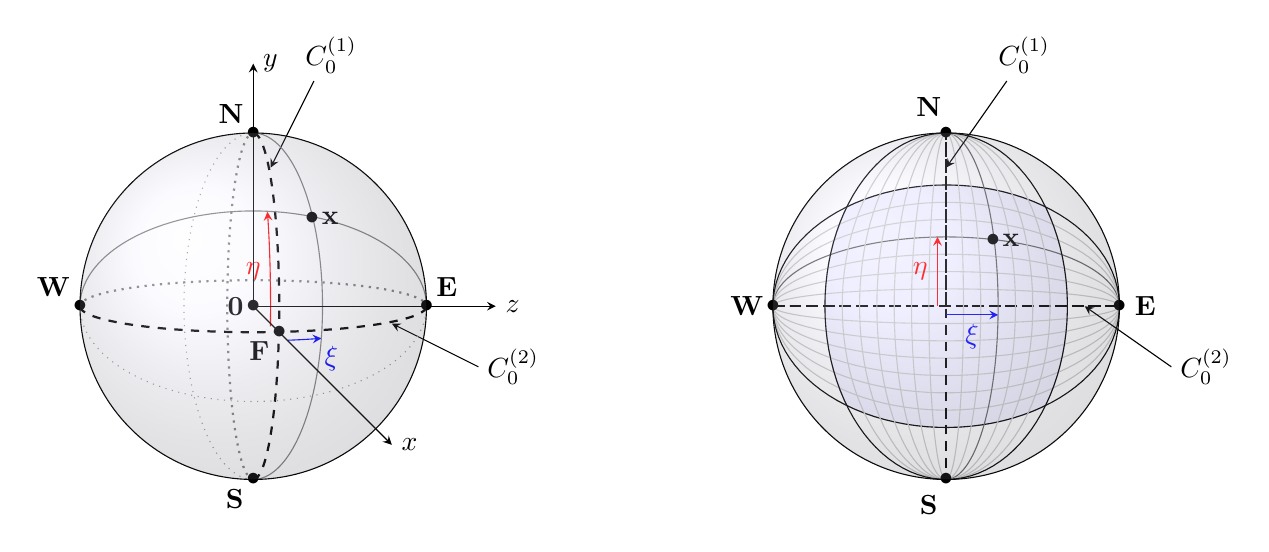
\begin{tikzpicture}[scale=2.2]
    \draw[>=stealth, ->, samples=100, color=blue, domain=-79:-68] plot({1.05*cos(\x)},{0.2*sin(\x)});
    \draw[color=blue] (.45,-.3) node{$\xi$} ;
    \draw[>=stealth, ->, samples=100, color=red, domain=-7:35] plot({0.1*cos(\x)},{0.95*sin(\x)});
    \draw[color=red] (0,0.2) node{$\eta$} ;

	\draw [dashed, line width=0.8pt, samples=100, domain=-180:0] plot({cos(\x)},{0.15*sin(\x)});
	\draw [dotted, line width=0.8pt, samples=100, domain=-180:0, color=gray] plot({cos(\x)},{-0.15*sin(\x)});
	\draw [dashed, line width=0.8pt, samples=100,domain=-90:90] plot({0.15*cos(\x)},{sin(\x)});
	\draw [dotted, line width=0.8pt, samples=100,domain=-90:90, color=gray] plot({-0.15*cos(\x)},{sin(\x)});
	\draw [>=stealth, ->] (1.3,-.35) -- (0.8,-0.1) ;
	\draw  (1.5,-.35) node {$C_0^{(2)}$} ;
	\draw [>=stealth, ->] (0.35,1.3) -- (0.1,0.8) ;
	\draw  (.45,1.45) node {$C_0^{(1)}$} ;
    
    
	\draw [samples=100, domain=-180:0, color=gray] plot({cos(\x)},{-0.55*sin(\x)});
	\draw [dotted, samples=100, domain=-180:0, color=gray!80] plot({cos(\x)},{0.55*sin(\x)});
	\draw [samples=100, domain=-90:90, color=gray] plot({0.4*cos(\x)},{sin(\x)});
	\draw [dotted, samples=100, domain=-90:90, color=gray!80] plot({-0.4*cos(\x)},{sin(\x)});
	\draw (.34,0.51) node {$\bullet$} ;
	\draw (.34,0.51) node[right]{$\mathbf{x}$} ;
	
	\draw (1,0) node {$\bullet$} ;
	\draw (1,0) node[above right]{$\mathbf{E}$} ;
	\draw (-1,0) node {$\bullet$} ;
	\draw (-1,0) node[above left]{$\mathbf{W}$} ;
	\draw (0,1) node {$\bullet$} ;
	\draw (0,1) node[above left]{$\mathbf{N}$} ;
	\draw (0,-1) node {$\bullet$} ;
	\draw (0,-1) node[below left]{$\mathbf{S}$} ;
	\draw (.15,-0.15) node {$\bullet$} ;
	\draw (.15,-0.15) node[below left]{$\mathbf{F}$} ;
	\draw (0,0) node {$\bullet$} ;
	\draw (0,0) node[left]{$\mathbf{0}$} ;
	
	\draw [>=stealth, ->] (0,0) -- (0,1.4) ;
	\draw  (0,1.4) node[right] {$y$} ;
	\draw [>=stealth, ->] (0,0) -- (1.4,0) ;
	\draw  (1.4,0) node[right] {$z$} ;
	\draw [>=stealth, ->] (0,0) -- (.8,-0.8) ;
	\draw  (.8,-0.8) node[right] {$x$} ;
	
	
    \draw (0,0) circle (1cm);
    \shade[ball color=blue!10!white,opacity=0.20] (0,0) circle (1cm);
    
    
    
    
    
    
    \filldraw[draw=black,fill=blue!30!white,opacity=0.20]
	plot [smooth,domain=-35:35] ({4+0.7*cos(\x)},{sin(\x)})
	-- plot [smooth,domain=55:125] ({4+cos(\x)},{0.7*sin(\x)})
	-- plot [smooth,domain=140:215] ({4+0.7*cos(\x)},{sin(\x)})
	-- plot [smooth,domain=230:305] ({4+cos(\x)},{0.7*sin(\x)})
	-- cycle;	
	
	\draw [dashed, line width=0.8pt, samples=100,domain=180:-180] plot({4+cos(\x)},{0*sin(\x)});
	\draw [samples=100,domain=180:-180,color=gray!40] plot({4+cos(\x)},{0.1*sin(\x)});
	\draw [samples=100,domain=180:-180,color=gray!40] plot({4+cos(\x)},{0.2*sin(\x)});
	\draw [samples=100,domain=180:-180,color=gray!40] plot({4+cos(\x)},{0.3*sin(\x)});
	\draw [samples=100,domain=180:0,color=gray!120] plot({4+cos(\x)},{0.4*sin(\x)});
	\draw [samples=100,domain=0:-180,color=gray!40] plot({4+cos(\x)},{0.4*sin(\x)});
	\draw [samples=100,domain=180:-180,color=gray!40] plot({4+cos(\x)},{0.5*sin(\x)});
	\draw [samples=100,domain=180:-180,color=gray!40] plot({4+cos(\x)},{0.6*sin(\x)});
	\draw [samples=100,domain=180:-180] plot({4+cos(\x)},{0.7*sin(\x)});
	\draw [dashed, line width=0.8pt, samples=100,domain=180:-180] plot({4+0*cos(\x)},{sin(\x)});
	\draw [samples=100,domain=180:-180,color=gray!40] plot({4+0.1*cos(\x)},{sin(\x)});
	\draw [samples=100,domain=180:-180,color=gray!40] plot({4+0.2*cos(\x)},{sin(\x)});
	\draw [samples=100,domain=-90:90,color=gray!120] plot({4+0.3*cos(\x)},{sin(\x)});
	\draw [samples=100,domain=90:270,color=gray!40] plot({4+0.3*cos(\x)},{sin(\x)});
	\draw [samples=100,domain=180:-180,color=gray!40] plot({4+0.4*cos(\x)},{sin(\x)});
	\draw [samples=100,domain=180:-180,color=gray!40] plot({4+0.5*cos(\x)},{sin(\x)});
	\draw [samples=100,domain=180:-180,color=gray!40] plot({4+0.6*cos(\x)},{sin(\x)});
	\draw [samples=100,domain=180:-180] plot({4+0.7*cos(\x)},{sin(\x)}); 
	
	\draw [>=stealth, ->] (5.3,-.35) -- (4.8,-0) ;
	\draw  (5.5,-.35) node {$C_0^{(2)}$} ;
	\draw [>=stealth, ->] (4.35,1.3) -- (4,0.8) ;
	\draw  (4.45,1.45) node {$C_0^{(1)}$} ;
	\draw  (4,1) node {$\bullet$} ;
	\draw  (3.9,1.15) node {$\mathbf{N}$} ;
	\draw  (4,-1) node {$\bullet$} ;
	\draw  (3.9,-1.15) node {$\mathbf{S}$} ;
	\draw  (5,0) node {$\bullet$} ;
	\draw  (5.15,0) node {$\mathbf{E}$} ;
	\draw  (3,0) node {$\bullet$} ;
	\draw  (4-1.15,0) node {$\mathbf{W}$} ;
	
	\draw  (4.27,0.38) node {$\bullet$} ;
	\draw  (4.27,0.38) node[right] {$\mathbf{x}$} ;
	\draw [>=stealth, ->, color=blue] (4,-0.05) -- (4.3,-0.05) ;
	\draw  (4.15,-0.05) node[color=blue, below] {$\xi$} ;
	\draw [>=stealth, ->, color=red] (3.95,0) -- (3.95,0.4) ;
	\draw  (3.95,0.2) node[color=red, left] {$\eta$} ;

	\draw (4,0) circle (1cm);
    \shade[ball color=blue!10!white,opacity=0.20] (4,0) circle (1cm);  
   
\end{tikzpicture}
\end{center}
\caption{Sur un panel, un point $\mathbf{x}$ est localisé par $\xi$ et $\eta$.}
\label{fig: panel I xi eta}
\end{figure}


On note $C^{(1)}_i$ le grand cercle obtenu par rotation de $C^{(1)}_0$ d'un angle géodésique $i \Delta \xi$ autour de l'axe $(Oz)$ et $C^{(2)}_j$ le cercle obtenu par rotation de $C^{(2)}_0$ d'angle $j \Delta \eta$ autour de $(Oy)$.

Le maillage associé au panel $(I)$ est constitué des points d'intersections des $N+1$ cercles $( C_i^{(1)} )_{-N/2 \leq i \leq N/2}$ et des $N+1$ cercles $(C_j^{(2)})_{-N/2 \leq j \leq N/2}$ (voir Figure \ref{fig: panel I}) sur le panel $(I)$. Le même procédé est reproduit sur chaque panel, il y a donc $(N+1)^2$ points d'intersections sur un panel.

\begin{figure}[htbp]
\begin{center}
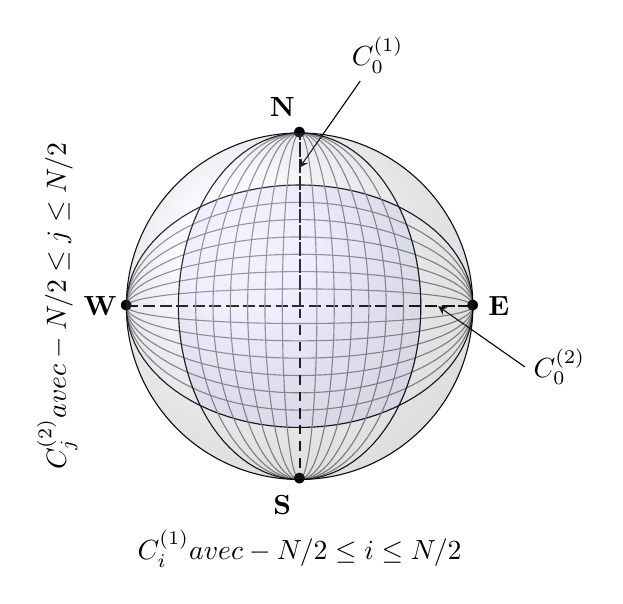
\begin{tikzpicture}[scale=2.2]
	%\draw [color=gray] (-2.5,-2.5) grid[step=0.1] (2.5,2.5);
	\filldraw[draw=black,fill=blue!30!white,opacity=0.20]
	plot [smooth,domain=-35:35] ({0.7*cos(\x)},{sin(\x)})
	-- plot [smooth,domain=55:125] ({cos(\x)},{0.7*sin(\x)})
	-- plot [smooth,domain=140:215] ({0.7*cos(\x)},{sin(\x)})
	-- plot [smooth,domain=230:305] ({cos(\x)},{0.7*sin(\x)})
	-- cycle;	
	
	\draw [dashed, line width=0.8pt, samples=100,domain=180:-180] plot({cos(\x)},{0*sin(\x)});
	\draw [samples=100,domain=180:-180,color=gray] plot({cos(\x)},{0.1*sin(\x)});
	\draw [samples=100,domain=180:-180,color=gray] plot({cos(\x)},{0.2*sin(\x)});
	\draw [samples=100,domain=180:-180,color=gray] plot({cos(\x)},{0.3*sin(\x)});
	\draw [samples=100,domain=180:-180,color=gray] plot({cos(\x)},{0.4*sin(\x)});
	\draw [samples=100,domain=180:-180,color=gray] plot({cos(\x)},{0.5*sin(\x)});
	\draw [samples=100,domain=180:-180,color=gray] plot({cos(\x)},{0.6*sin(\x)});
	\draw [samples=100,domain=180:-180] plot({cos(\x)},{0.7*sin(\x)});
	\draw [dashed, line width=0.8pt, samples=100,domain=180:-180] plot({0*cos(\x)},{sin(\x)});
	\draw [samples=100,domain=180:-180,color=gray] plot({0.1*cos(\x)},{sin(\x)});
	\draw [samples=100,domain=180:-180,color=gray] plot({0.2*cos(\x)},{sin(\x)});
	\draw [samples=100,domain=180:-180,color=gray] plot({0.3*cos(\x)},{sin(\x)});
	\draw [samples=100,domain=180:-180,color=gray] plot({0.4*cos(\x)},{sin(\x)});
	\draw [samples=100,domain=180:-180,color=gray] plot({0.5*cos(\x)},{sin(\x)});
	\draw [samples=100,domain=180:-180,color=gray] plot({0.6*cos(\x)},{sin(\x)});
	\draw [samples=100,domain=180:-180] plot({0.7*cos(\x)},{sin(\x)}); 
	
	\draw [>=stealth, ->] (1.3,-.35) -- (0.8,-0) ;
	\draw  (1.5,-.35) node {$C_0^{(2)}$} ;
	\draw [>=stealth, ->] (0.35,1.3) -- (0,0.8) ;
	\draw  (0.45,1.45) node {$C_0^{(1)}$} ;
	\draw  (0,1) node {$\bullet$} ;
	\draw  (-0.1,1.15) node {$\mathbf{N}$} ;
	\draw  (0,-1) node {$\bullet$} ;
	\draw  (-0.1,-1.15) node {$\mathbf{S}$} ;
	\draw  (1,0) node {$\bullet$} ;
	\draw  (1.15,0) node {$\mathbf{E}$} ;
	\draw  (-1,0) node {$\bullet$} ;
	\draw  (-1.15,0) node {$\mathbf{W}$} ;

	\draw (0,0) circle (1cm);
    \shade[ball color=blue!10!white,opacity=0.20] (0,0) circle (1cm);
    
    \draw  (-1.4,0) node[rotate=90] {$ C_j^{(2)}\text{ avec }-N/2\leq j \leq N/2$} ;
    \draw  (0,-1.4) node {$ C_i^{(1)}\text{ avec }-N/2\leq i \leq N/2$} ;

\end{tikzpicture}
\end{center}
\caption{Le panel $(I)$ est constitué des points d'intersections d'un ensemble de grands cercles.}
\label{fig: panel I}
\end{figure}  

En reproduisant le procédé pour chaque panel, on constitue la Cubed-Sphere associée à la base $(\mathbf{i},\mathbf{j},\mathbf{k})$ et de paramètre $N \in \mathbb{N}^{\star}$.

\begin{definition}
La Cubed-Sphere est une grille de la sphère $\mathbb{S}_a^2$. La sphère est couverte par 6 panels identiques notés panel $(I)$ (Front), $(II)$ (East), $(III)$ (Bottom), $(IV)$ (West), $(V)$ (North) et $(VI)$ (South). Chaque panel est doté d'un système de coordonnées :
\begin{equation}
\left( \xi^{(k)}, \eta^{(k)} \right) \text{, } -\dfrac{\pi}{4} \leq \xi^{(k)}, \eta^{(k)} \leq \dfrac{\pi}{4} \text{, } (I) \leq (k) \leq (VI)
\end{equation}
défini précédemment. Les points de la Cubed-Sphere sont notés $\mathbf{x}_{i,j}^{(k)}$. Ils sont définis par leurs coordonnées $\left( \xi_i^{(k)}, \eta_j^{(k)}  \right)$ avec :
\begin{equation}
\xi_i^{(k)} = i \Delta \xi \text{, } \eta_j^{(k)} = j \Delta \eta \text{, } -N/2 \leq i, j \leq N/2 \text{ et } (I) \leq (k) \leq (VI),
\end{equation}
où le pas de discrétisation est :
\begin{equation}
\Delta \xi = \Delta \eta = \dfrac{\pi}{2 N}.
\end{equation}
\end{definition}

\begin{proposition}
La Cubed-Sphere est composée de $6N^2 +2$ points.
\end{proposition}

\begin{proof}
Il y a 6 intérieurs de panels de $(N-1)^2$ points, 12 arrêtes de $N-1$ points et 8 sommets. Ainsi le nombre de points sur la Cubed-Sphere est :
\begin{equation}
6 (N-1)^2 + 12 (N-1)+8=6N^2+2.
\end{equation}
\end{proof}

Les points $\mathbf{x}_{i,j}^{(k)}$ de chaque panel se répartissent en trois catégories :
\begin{itemize}
\item Les points intérieurs si :
\begin{equation}
- \dfrac{N}{2}+1 \leq i,j \leq \dfrac{N}{2}-1
\end{equation}
Ils sont au nombre de $(N-1)^2$ par panel.
\item Les $4(N-1)$ points de bords de chaque panel, si :
\begin{equation}
\left[ j=\pm \dfrac{N}{2} \text{ et } - \dfrac{N}{2}+1 \leq i \leq \dfrac{N}{2}-1 \right] \text{ ou } \left[ i=\pm \dfrac{N}{2} \text{ et } - \dfrac{N}{2}+1 \leq j \leq \dfrac{N}{2}-1 \right]
\end{equation}
\item Les $4$ points de coins si :
\begin{equation}
i, j = \pm \dfrac{N}{2}.
\end{equation}
\end{itemize}



\begin{figure}
\begin{center}
\includegraphics[height=14.3cm]{plot_CS.jpg}
\end{center}
\caption{Cubed-Sphere avec $N=16$.}
\end{figure}















\section{Coordonnées Gnomoniques}
\label{sec:gnomonique}

On considère un cube inscrit dans la sphère $\mathbb{S}_a^2$. Le demi côté de ce cube mesure $R=\frac{\sqrt{3}}{3}a$. Chaque face du cube est donnée par :
\begin{itemize}
\item la face centrée sur $F'=(R,0,0)$ : 
\begin{equation}
\left\lbrace
\mathbf{x}' = (R,y',z') \in \mathbb{R}^3 \text{ tels que } -R  \leq y',z' \leq R
\right\rbrace
\end{equation}

\item la face centrée sur $B'=(-R,0,0)$ : 
\begin{equation}
\left\lbrace
\mathbf{x}' = (-R,y',z') \in \mathbb{R}^3 \text{ tels que } -R  \leq y',z' \leq R
\right\rbrace ,
\end{equation}

\item la face centrée sur $E'=(0,R,0)$ : 
\begin{equation}
\left\lbrace
\mathbf{x}' = (x',R,z') \in \mathbb{R}^3 \text{ tels que } -R  \leq x',z' \leq R
\right\rbrace ,
\end{equation}

\item la face centrée sur $W'=(0,-R,0)$ : 
\begin{equation}
\left\lbrace
\mathbf{x}' = (x',-R,z') \in \mathbb{R}^3 \text{ tels que } -R  \leq x',z' \leq R
\right\rbrace ,
\end{equation}

\item la face centrée sur $N'=(0,0,R)$ : 
\begin{equation}
\left\lbrace
\mathbf{x}' = (x',y',R) \in \mathbb{R}^3 \text{ tels que } -R  \leq x',y' \leq R
\right\rbrace ,
\end{equation}

\item la face centrée sur $S'=(0,0,-R)$ : 
\begin{equation}
\left\lbrace
\mathbf{x}' = (x',y',-R) \in \mathbb{R}^3 \text{ tels que } -R  \leq x',y' \leq R
\right\rbrace .
\end{equation}
\end{itemize}

Le point $\mathbf{F}$ est la projection gnomonique du point $F'$ sur la sphère $\mathbb{S}_a^2$, $\mathbf{E}$ celle de $E'$, etc.
Si l'on considère par exemple le panel $(I)$, un point $\mathbf{x}'=(x',y',z')$ de la face centrée sur $F'$ est projeté en $\mathbf{x} = (x,y,z)$ un point du panel $(I)$ (voir Fig. \ref{fig: projection gnomonique}). Chaque panel est la projection de l'une des faces du cube.

\begin{figure}[htbp]
\begin{center}
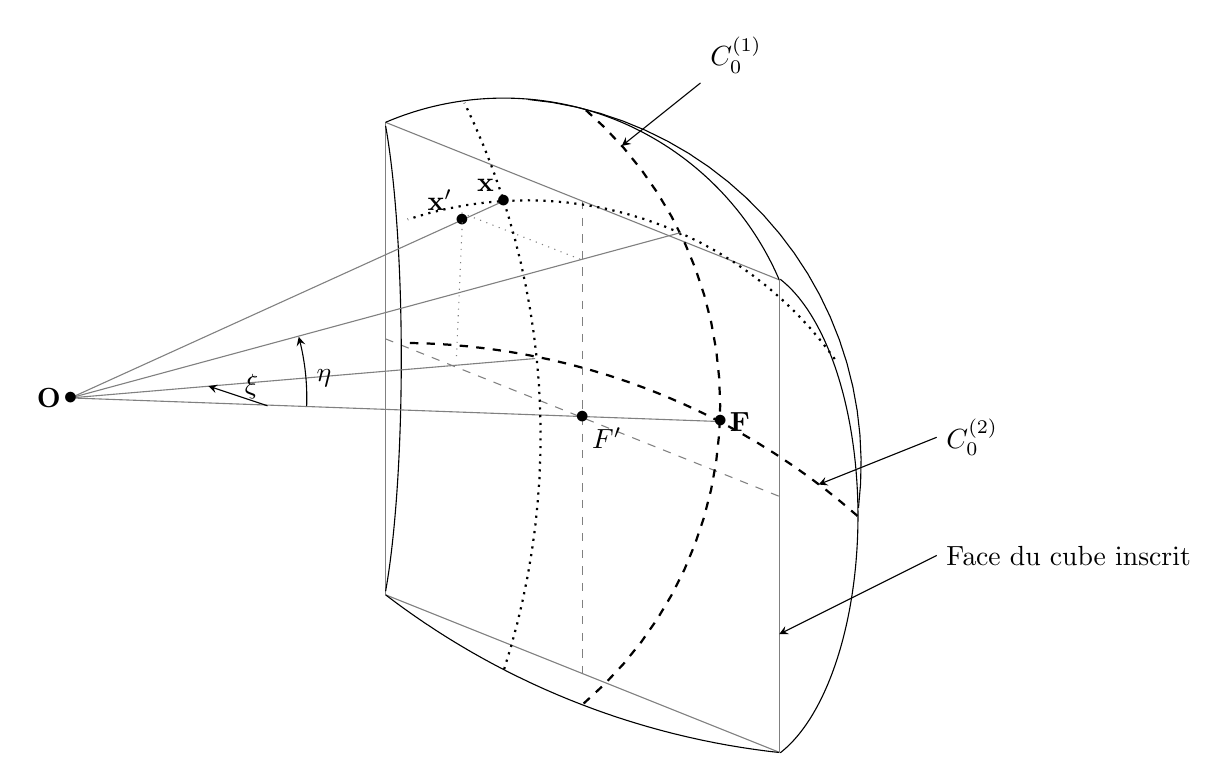
\begin{tikzpicture}[scale=1]
	\draw [color=gray] (0,3) -- (0,-3) ;
	\draw [color=gray] (0,-3) -- (5,-5) ;
	\draw [color=gray] (5,-5) -- (5,1) ;
	\draw [color=gray] (5,1) -- (0,3) ;
	\draw [dashed, color=gray] (0,.25) -- (5,-1.75) ;
	\draw [dashed, color=gray] (2.5,2) -- (2.5,-4) ;
	
	\draw [samples=100,domain=-70:70] plot({4.5+1.5*cos(\x)},{-2+3.2*sin(\x)});
	\draw [samples=100,domain=-53:53] plot({-0.3+0.5*cos(\x)},{3.7*sin(\x)});
	\draw [samples=100,domain=113.2:23.2] plot({1.5+sqrt(14.5)*cos(\x)},{-.5+sqrt(14.5)*sin(\x)});
	\draw [samples=100,domain=-96.24:-127.41] plot({6.09+sqrt(100.46)*cos(\x)},{4.96+sqrt(100.46)*sin(\x)});
	
	\draw [shift={(1.39,-1.34)}] plot[domain=-0.12:1.48,variable=\t]({1*4.65*cos(\t r)+0*4.65*sin(\t r)},{0*4.65*cos(\t r)+1*4.65*sin(\t r)});
	
	
	\draw [color=gray] (-4,-.5) -- (4.25,-0.8) ;
	\draw  (2.5,-.75) node {$\bullet$} ;
	\draw  (2.5,-.75) node[below right] {$F'$} ;
	\draw  (4.25,-0.8) node {$\bullet$} ;
	\draw  (4.25,-0.8) node[right] {$\mathbf{F}$} ;
	
	\draw [dashed, line width=0.8pt, shift={(-0.74,-0.6)}] plot[domain=-0.86:0.86,variable=\t]({1*4.99*cos(\t r)+0*4.99*sin(\t r)},{0*4.99*cos(\t r)+1*4.99*sin(\t r)});
	\draw [dashed, line width=0.8pt, shift={(0.16,-8.64)}] plot[domain=0.85:1.56,variable=\t]({1*8.84*cos(\t r)+0*8.84*sin(\t r)},{0*8.84*cos(\t r)+1*8.84*sin(\t r)});
	
	\draw [color=gray] (-4,-.5) -- (1.5,2) ;
	\draw  (1.5,2) node {$\bullet$} ;
	\draw  (1.5,2) node[above left] {$\textbf{x}$} ;
	
	\draw [dotted, line width=0.8pt, shift={(1.79,-2.8)}] plot[domain=0.62:1.89,variable=\t]({1*4.81*cos(\t r)+0*4.81*sin(\t r)},{0*4.81*cos(\t r)+1*4.81*sin(\t r)});
	\draw [dotted, line width=0.8pt, shift={(-7.75,-0.98)}] plot[domain=-0.31:0.45,variable=\t]({1*9.72*cos(\t r)+0*9.72*sin(\t r)},{0*9.72*cos(\t r)+1*9.72*sin(\t r)});

	\draw [color=gray] (-4,-.5) -- (1.9,0) ;
	\draw [color=gray] (-4,-.5) -- (3.75,1.6) ;
	
	\draw  (.97,1.75) node {$\bullet$} ;
	\draw  (.97,1.75) node[above left] {$\textbf{x}'$} ;
	\draw [dotted, color=gray] (.965,1.85) -- (2.5,1.25) ;
	\draw [dotted, color=gray] (.975,1.73) -- (.9,0) ;
	
	\draw  (-4,-.5) node {$\bullet$} ;
	\draw  (-4,-.5) node[left] {$\mathbf{O}$} ;
	
	\draw [>=stealth, ->] (-1.5,-.6) -- (-2.25,-.35) ;
	\draw  (-1.7,-.35) node {$\xi$} ;
	\draw [>=stealth, ->,domain=-2:15] plot({-4+3*cos(\x)},{-.5+3*sin(\x)});
	\draw  (-1,-.25) node[right] {$\eta$} ;
	
	\draw [>=stealth, <-] (5.5,-1.6) -- (7,-1) ;
	\draw  (7,-1) node[right] {$C_0^{(2)}$} ;
	\draw [>=stealth, <-] (3,2.7) -- (4,3.5) ;
	\draw  (4,3.5) node[above right] {$C_0^{(1)}$} ;
	\draw [>=stealth, <-] (5,-3.5) -- (7,-2.5) ;
	\draw  (7,-2.5) node[right] {Face du cube inscrit} ;

\end{tikzpicture}
\end{center}
\caption{Projection gnomonique.}
\label{fig: projection gnomonique}
\end{figure}  

On a les relations suivantes :
\begin{equation}
\tan \xi = \dfrac{y'}{x'} = \dfrac{y}{x} \text{ et } \tan \eta = \dfrac{z'}{x'} = \dfrac{z}{x}
\end{equation}
Or $\mathbf{x}'(x',y',z')$ est un point de la face du cube centrée en $F'$, donc $x'=R=\frac{\sqrt{3}}{3}a$ :
\begin{equation}
\tan \xi = \dfrac{y'}{R} = \dfrac{y}{x} \text{ et } \tan \eta = \dfrac{z'}{R} = \dfrac{z}{x}
\end{equation}
Sur chaque panel, on définit les coordonnées gnomoniques $(X,Y)$ par :

\begin{definition}
Les coordonnées gnomoniques $(X,Y) \in [-1,1]^2$ sont définies par :
\begin{equation}
X=\tan \xi \text{ et } Y= \tan \eta.
\end{equation}
\end{definition}

Un point de la sphère est localisé de manière unique par sa face et ses coordonnées gnomoniques. Si on se donne $(X,Y)$ un couple de coordonnées gnomoniques du panel $(I)$, on a :

\begin{eqsys}
x^2+y^2+z^2 = a^2\\
X = \dfrac{y}{x} \\
Y = \dfrac{z}{x}
\end{eqsys}
ainsi $x^2 \left( 1+X^2+Y^2 \right) = a^2$, d'où :
\begin{equation}
\left\lbrace
\begin{array}{rclcl}
x & = & \pm \dfrac{a}{\sqrt{1+X^2+Y^2}}& = & \dfrac{a}{\sqrt{1+X^2+Y^2}}\\
y & = & xX &&\\
z & = & xY. &&
\end{array}
\right.
\end{equation}

Le signe de $x$ est prescrit car $\mathbf{x}$ est un point du panel $(I)$ qui ne contient que des points d'abscisse positive.
De plus, la fonction $\tan$ est une bijection de $\left[ -\dfrac{\pi}{4}, \dfrac{\pi}{4} \right]$ dans $\left[-1,1\right]$, donc

\begin{theoreme}
Pour chaque panel, les coordonnées gnomoniques $(X,Y) \in [-1,1]^2$ et $(\xi, \eta) \in \left[ - \dfrac{\pi}{4}, \dfrac{\pi}{4} \right]^2$ forment deux systèmes de coordonnées admissibles.
\end{theoreme}
On peut dériver les coordonnées d'un point $\mathbf{x}(x,y,z) \in \mathbb{R}^3$ en fonction de $\xi$ et $\eta$ :

\begin{equation}
\dfrac{\partial y}{\partial \xi} = \dfrac{\partial x}{\partial \xi} X + x \dfrac{\partial X}{\partial \xi} = \dfrac{\partial x}{\partial \xi} X + x(1+X^2)
\end{equation}

\begin{equation}
\dfrac{\partial z}{\partial \xi} = \dfrac{\partial x}{\partial \xi} Y + x \dfrac{\partial Y}{\partial \xi} = \dfrac{\partial x}{\partial \xi} Y .
\end{equation}
Le calcul de ces dérivées dépend de $\dfrac{\partial x}{\partial \xi}$ :

\begin{equation*}
\begin{array}{rcl}
0 & = & \dfrac{\partial}{\partial \xi} ( x^2+y^2+z^2) \\
  & = & 2x\dfrac{\partial x}{\partial \xi} + 2y\dfrac{\partial y}{\partial \xi}+ 2z\dfrac{\partial z}{\partial \xi} \\
  & = & x \dfrac{\partial x}{\partial \xi} ( 1 +X^2 + Y^2) + x^2 X (1+X^2)\\
  & = & x \dfrac{\partial x}{\partial \xi} \delta^2 + xy (1+X^2),
\end{array}
\end{equation*}
en posant $\delta = \sqrt{1+X^2+Y^2}$. Ainsi, chaque dérivée est connue et :

\begin{equation}
\left\lbrace
\begin{array}{rcl}
\dfrac{\partial x}{\partial \xi} & = & -\dfrac{y(1+X^2)}{\delta^2}\\
\dfrac{\partial y}{\partial \xi} & = & x \dfrac{1+X^2}{\delta^2} (1+Y^2)\\
\dfrac{\partial z}{\partial \xi} & = & - \dfrac{yY(1+X^2)}{\delta^2} .
\end{array}
\right.
\end{equation}
De la même manière, en dérivant par rapport à $\eta$ :
\begin{equation}
\left\lbrace
\begin{array}{rcl}
\dfrac{\partial x}{\partial \eta} & = & - z\dfrac{1+Y^2}{\delta^2}\\
\dfrac{\partial y}{\partial \eta} & = & - zX\dfrac{1+Y^2}{\delta^2}\\
\dfrac{\partial z}{\partial \eta} & = & - x(1+X^2) \dfrac{1+Y^2}{\delta^2}.
\end{array}
\right.
\end{equation}

On en déduit la base sur le panel $(I)$ : $\left( \mathbf{g}_{\xi}, \mathbf{g}_{\eta} \right)$, donnée par :

\begin{equation}
\mathbf{g}_{\xi} = \dfrac{\partial \mathbf{x}}{\partial \xi}= \dfrac{1+X^2}{\delta^2} \begin{bmatrix}
-y \\ x(1+Y^2) \\ -yY
\end{bmatrix} \text{ et } \mathbf{g}_{\eta} = \dfrac{\partial \mathbf{x}}{\partial \xi}= \dfrac{1+Y^2}{\delta^2} \begin{bmatrix}
-z \\ -zX \\ x(1+X^2)
\end{bmatrix} .
\label{eq: base locale I}
\end{equation}

Des calculs similaires peuvent être effectuées sur les autres panels. Les résultats sont donnés dans la Table \ref{tab: base g_xi g_eta}.

Le couple de vecteurs $(\mathbf{g}^{\xi}, \mathbf{g}^{\eta})$ est la base duale de $(\mathbf{g}_{\xi}, \mathbf{g}_{\eta})$. Cette base doit vérifier les relations suivantes :
\begin{equation}
\left\lbrace
\begin{array}{rcccl}
\mathbf{g}^{\xi} \cdot \mathbf{g}_{\xi} & = & 1 & = & \mathbf{g}^{\eta} \cdot \mathbf{g}_{\eta} \\
\mathbf{g}^{\xi} \cdot \mathbf{g}_{\eta} & = & 0 & = & \mathbf{g}^{\eta} \cdot \mathbf{g}_{\xi}. \\
\end{array}
\right.
\label{eq: normalisation g_xi g_eta}
\end{equation}
Les vecteurs $\mathbf{g}^{\xi}$ et $\mathbf{g}^{\eta}$ sont des vecteurs de $\mathbb{T}_{\mathbf{x}}\mathbb{S}_a^2$. Il existe $A$, $B$, $C$ et $D$ tels que :
\begin{equation}
\left\lbrace
\begin{array}{rcl}
\mathbf{g}^{\xi} & = & A \mathbf{g}_{\xi} + B \mathbf{g}_{\eta} \\
\mathbf{g}^{\eta} & = & C \mathbf{g}_{\xi} + D \mathbf{g}_{\eta} \\
\end{array}
\right.
\label{eq: A B C D}
\end{equation}
En effectuant des produit scalaires de \eqref{eq: A B C D} par $\mathbf{g}_{\xi}$ et $\mathbf{g}_{\eta}$, on obtient :
\begin{equation}
\begin{bmatrix}
A & B \\ C &  D
\end{bmatrix}
\times
\begin{bmatrix}
\mathbf{g}_{\xi} \cdot \mathbf{g}_{\xi} & \mathbf{g}_{\xi} \cdot \mathbf{g}_{\eta} \\
\mathbf{g}_{\eta} \cdot \mathbf{g}_{\xi} & \mathbf{g}_{\eta} \cdot \mathbf{g}_{\eta}
\end{bmatrix}
= \begin{bmatrix}
1 & 0 \\ 0 &  1
\end{bmatrix}.
\end{equation}
On en déduit :
\begin{equation}
\begin{bmatrix}
A & B \\ C &  D
\end{bmatrix} 
=
\begin{bmatrix}
\mathbf{g}_{\xi} \cdot \mathbf{g}_{\xi} & \mathbf{g}_{\xi} \cdot \mathbf{g}_{\eta} \\
\mathbf{g}_{\eta} \cdot \mathbf{g}_{\xi} & \mathbf{g}_{\eta} \cdot \mathbf{g}_{\eta}
\end{bmatrix}^{-1}.
\end{equation}


\begin{definition}
La matrice $\mathbf{G}$ est la métrique associée à $(\mathbf{g}_{\xi}, \mathbf{g}_{\eta})$ en $\mathbf{x}$:
\begin{equation}
\mathbf{G} = \begin{bmatrix}
\mathbf{g}_{\xi} \cdot \mathbf{g}_{\xi} & \mathbf{g}_{\xi} \cdot \mathbf{g}_{\eta} \\
\mathbf{g}_{\eta} \cdot \mathbf{g}_{\xi} & \mathbf{g}_{\eta} \cdot \mathbf{g}_{\eta}
\end{bmatrix} .
\end{equation}
\end{definition}

\begin{proposition}
La métrique $\mathbf{G}$ est invariante par changement de panel.
\end{proposition}

\begin{proof}
Soit $\mathbf{x}$ un point d'un panel $(k)$ de la Cubed-Sphere de coordonnées gnomoniques $(X,Y)$ et $\mathbf{x}'$ un point d'un autre panel $(k')$ de la Cubed-Sphere ayant les mêmes coordonnées gnomoniques $(X,Y)$. Il existe une rotation $R_f$ qui permet de transformer tout point du panel $(k)$ en un point du panel $(k')$ de mêmes coordonnées gnomoniques. De là, il découle :
\begin{equation}
\mathbf{x}' = R_f \mathbf{x}.
\end{equation}
Cette rotation est indépendante de $\xi$ et de $\eta$. Donc :
\begin{equation}
\mathbf{g'}_{\xi} = \dfrac{\partial}{\partial \xi} \left( R_f \mathbf{x} \right) = R_f \dfrac{\partial \mathbf{x}}{\partial \xi}  = R_f \mathbf{g}_{\xi}.
\end{equation}
De même, on a $\mathbf{g'}_{\eta} = R_f\mathbf{g}_{\eta}$.
Ainsi, si $\mathbf{G}$ est la métrique en $\mathbf{x}$ et $\mathbf{G}'$ la métrique en $\mathbf{x}'$, on a :

\begin{equation*}
\begin{array}{rcl}
\mathbf{G}' &=& \begin{bmatrix}
\mathbf{g'}_{\xi} \cdot \mathbf{g'}_{\xi} & \mathbf{g'}_{\xi} \cdot \mathbf{g'}_{\eta} \\
\mathbf{g'}_{\eta} \cdot \mathbf{g'}_{\xi} & \mathbf{g'}_{\eta} \cdot \mathbf{g'}_{\eta}
\end{bmatrix}\\[10pt]
&=&
\begin{bmatrix}
R_f \mathbf{g}_{\xi} \cdot R_f \mathbf{g}_{\xi} & R_f \mathbf{g}_{\xi} \cdot R_f \mathbf{g}_{\eta} \\
R_f \mathbf{g}_{\eta} \cdot R_f \mathbf{g}_{\xi} & R_f \mathbf{g}_{\eta} \cdot R_f \mathbf{g}_{\eta}
\end{bmatrix}\\[10pt]
&=&
\begin{bmatrix}
\mathbf{g}_{\xi} \cdot R_f^{T} R_f \mathbf{g}_{\xi} & \mathbf{g}_{\xi} \cdot  R_f^{T} R_f \mathbf{g}_{\eta} \\
\mathbf{g}_{\eta} \cdot  R_f^{T} R_f \mathbf{g}_{\xi} & \mathbf{g}_{\eta} \cdot  R_f^{T} R_f \mathbf{g}_{\eta}
\end{bmatrix}\\[10pt]
&=& \begin{bmatrix}
\mathbf{g}_{\xi} \cdot \mathbf{g}_{\xi} & \mathbf{g}_{\xi} \cdot \mathbf{g}_{\eta} \\
\mathbf{g}_{\eta} \cdot \mathbf{g}_{\xi} & \mathbf{g}_{\eta} \cdot \mathbf{g}_{\eta}
\end{bmatrix}\\[10pt]
& = & \mathbf{G}.
\end{array}
\end{equation*}
Donc la métrique $\mathbf{G}$ est invariante par changement de panel.
\end{proof}
L'expression de la métrique $\mathbf{G}$ en fonction de $(X,Y)$ est
\begin{equation}
\mathbf{G} = \begin{bmatrix}
G_{1,1} & G_{1,2} \\ G_{2,1} & G_{2,2}
\end{bmatrix} 
= a^2 \dfrac{(1+X^2)(1+Y^2)}{\delta^4} \begin{bmatrix}
1+X^2 & -XY \\ -XY & 1+Y^2
\end{bmatrix} .
\end{equation}
De même, on a
\begin{equation}
\mathbf{G}^{-1} = \begin{bmatrix}
G^{1,1} & G^{1,2} \\ G^{2,1} & G^{2,2}
\end{bmatrix} = \dfrac{\delta^2}{a^2 (1+X^2)(1+Y^2)} \begin{bmatrix}
1+Y^2 & XY \\ XY & 1+X^2
\end{bmatrix} .
\label{eq: metrique inverse}
\end{equation}
La base duale $(\mathbf{g}^{\xi}, \mathbf{g}^{\eta})$ sur le panel $(I)$ est donnée par :
\begin{equation}
\left\lbrace
\begin{array}{rcl}
\mathbf{g}^{\xi} & = & G^{1,1} \mathbf{g}_{\xi} + G^{1,2} \mathbf{g}_{\eta} \\
\mathbf{g}^{\eta} & = & G^{2,1} \mathbf{g}_{\eta} + G^{2,2} \mathbf{g}_{\eta}
\end{array}
\right.
\end{equation}
d'où :
\begin{equation}
\mathbf{g}^{\xi} = \dfrac{1}{x(1+X^2)}\begin{bmatrix}
-X \\ 1 \\ 0
\end{bmatrix} \text{ et } \mathbf{g}^{\eta} = \dfrac{1}{x(1+Y^2)}\begin{bmatrix}
-Y \\ 0 \\ 1
\end{bmatrix} .
\label{eq: base duale I}
\end{equation}



\begin{table}[htbp]
\begin{center}
%\rotatebox{90}{
\begin{tabular}{|c|c|c|}
\hline
\textbf{Panel} & \textbf{Coord. Gnomoniques} $(X,Y)$ & \textbf{Bases } $\left( \mathbf{g}_{\xi}, \mathbf{g}_{\eta} \right)$ et $\left( \mathbf{g}^{\xi}, \mathbf{g}^{\eta} \right)$\\

\hline
\hline
\multirow{2}{*}[-.5cm]{$(I)$} & \multirow{2}{*}[-.5cm]{$X=\dfrac{y}{x} \text{, } Y=\dfrac{z}{x}$} & $\mathbf{g}_{\xi} = \dfrac{1+X^2}{\delta^2} \begin{bmatrix}
-y \\ x(1+Y^2) \\ -yY
\end{bmatrix} \text{,} \mathbf{g}_{\eta} = \dfrac{1+Y^2}{\delta^2} \begin{bmatrix}
-z \\ -zX \\ x(1+X^2)
\end{bmatrix}$ \\[16pt]

\cline{3-3}
& &  $\mathbf{g}^{\xi} = \dfrac{1}{x(1+X^2)}\begin{bmatrix}
-X \\ 1 \\ 0
\end{bmatrix} \text{ et } \mathbf{g}^{\eta} = \dfrac{1}{x(1+Y^2)}\begin{bmatrix}
-Y \\ 0 \\ 1
\end{bmatrix}$ \\[16pt]
\hline
\hline
\multirow{2}{*}[-.5cm]{$(II)$} & \multirow{2}{*}[-.5cm]{$X=-\dfrac{x}{y} \text{, } Y=\dfrac{z}{y}$} & $\mathbf{g}_{\xi} = \dfrac{1+X^2}{\delta^2} \begin{bmatrix}
-y(1+Y^2) \\ x \\ xY
\end{bmatrix} \text{, } \mathbf{g}_{\eta} = \dfrac{1+Y^2}{\delta^2} \begin{bmatrix}
zX \\ -z \\ y(1+X^2)
\end{bmatrix}$ \\[16pt]

\cline{3-3}
 & & $\mathbf{g}^{\xi} = \dfrac{1}{y(1+X^2)}\begin{bmatrix}
-1 \\ -X \\ 0
\end{bmatrix} \text{, } \mathbf{g}^{\eta} = \dfrac{1}{y(1+Y^2)}\begin{bmatrix}
0 \\ -Y \\ 1
\end{bmatrix}$ \\[16pt]
\hline
\hline
\multirow{2}{*}[-.5cm]{$(III)$} & \multirow{2}{*}[-.5cm]{$X=-\dfrac{y}{x} \text{, } Y=-\dfrac{z}{x}$} & $\mathbf{g}_{\xi} = \dfrac{1+X^2}{\delta^2} \begin{bmatrix}
-y \\ x(1+Y^2) \\ yY
\end{bmatrix} \text{, } \mathbf{g}_{\eta} = \dfrac{1+Y^2}{\delta^2} \begin{bmatrix}
-z \\ -zX \\ x(1+X^2)
\end{bmatrix}$ \\[16pt]

 \cline{3-3}
 &  & $\mathbf{g}^{\xi} = \dfrac{1}{x(1+X^2)}\begin{bmatrix}
-X \\ 1 \\ 0
\end{bmatrix} \text{, } \mathbf{g}^{\eta} = \dfrac{1}{x(1+Y^2)}\begin{bmatrix}
-Y \\ 0 \\ -1
\end{bmatrix}$ \\[16pt]
\hline
\hline
\multirow{2}{*}[-.5cm]{$(IV)$} & \multirow{2}{*}[-.5cm]{$X=\dfrac{x}{y} \text{, } Y=-\dfrac{z}{y}$} & $\mathbf{g}_{\xi} = \dfrac{1+X^2}{\delta^2} \begin{bmatrix}
-y(1+Y^2) \\ x \\ -xY
\end{bmatrix} \text{, } \mathbf{g}_{\eta} = \dfrac{1+Y^2}{\delta^2} \begin{bmatrix}
-zX \\ z \\ -y(1+X^2)
\end{bmatrix}$ \\[16pt]

\cline{3-3}
&  & $\mathbf{g}^{\xi} = \dfrac{1}{y(1+X^2)}\begin{bmatrix}
-1 \\ -X \\ 0
\end{bmatrix} \text{, } \mathbf{g}^{\eta} = \dfrac{1}{y(1+Y^2)}\begin{bmatrix}
0 \\ -Y \\ -1
\end{bmatrix}$ \\[16pt]
\hline
\hline
\multirow{2}{*}[-.5cm]{$(V)$} & \multirow{2}{*}[-.5cm]{$X=\dfrac{y}{z} \text{, } Y=\dfrac{x}{z}$} & $\mathbf{g}_{\xi} = \dfrac{1+X^2}{\delta^2} \begin{bmatrix}
-yY \\ z(1+Y^2) \\ -y
\end{bmatrix} \text{, } \mathbf{g}_{\eta} = \dfrac{1+Y^2}{\delta^2} \begin{bmatrix}
-z(1+X^2) \\ xX \\ x
\end{bmatrix}$ \\[16pt]

\cline{3-3}
 &  & $\mathbf{g}^{\xi} = \dfrac{1}{z(1+X^2)}\begin{bmatrix}
0 \\ 1 \\ -X
\end{bmatrix} \text{, } \mathbf{g}^{\eta} = \dfrac{1}{z(1+Y^2)}\begin{bmatrix}
-1 \\ 0 \\ -Y
\end{bmatrix}$ \\[16pt]
\hline
\hline
\multirow{2}{*}[-.5cm]{$(VI)$} & \multirow{2}{*}[-.5cm]{$X=-\dfrac{y}{z} \text{, } Y=-\dfrac{x}{z}$} & $\mathbf{g}_{\xi} = \dfrac{1+X^2}{\delta^2} \begin{bmatrix}
-yY \\ -z(1+Y^2) \\ y
\end{bmatrix} \text{, } \mathbf{g}_{\eta} = \dfrac{1+Y^2}{\delta^2} \begin{bmatrix}
-z(1+X^2) \\ -xX \\ x
\end{bmatrix}$ \\[16pt]

\cline{3-3}
 &  & $\mathbf{g}^{\xi} = \dfrac{1}{z(1+X^2)}\begin{bmatrix}
0 \\ -1 \\ -X
\end{bmatrix} \text{, } \mathbf{g}^{\eta} = \dfrac{1}{z(1+Y^2)}\begin{bmatrix}
-1 \\ 0 \\ -Y
\end{bmatrix}$ \\[16pt]
\hline

\end{tabular}
%}
\end{center}
\caption{Coordonnées gnomoniques en fonction de $x$, $y$ et $z$ et bases $\left( \mathbf{g}_{\xi}, \mathbf{g}_{\eta} \right)$ et $\left( \mathbf{g}^{\xi}, \mathbf{g}^{\eta} \right)$ en fonction de $x$, $y$ et $z$  sur chaque panel, avec $\delta=\sqrt{1+X^2+Y^2}$.}
\label{tab: base g_xi g_eta}
\end{table}

Les champs de vecteur $( \mathbf{g}^{\xi}, \mathbf{g}^{\eta})$ et $( \mathbf{g}_ {\xi}, \mathbf{g}_{\eta})$ sont tangents à la sphère et sont fonctions de $\xi$ et $\eta$. On définit les \textit{symboles de Christoffel} par :

\begin{definition}
Les symboles de Christoffel $\Gamma_{\kappa,\nu}^{\tau}$ (avec $\kappa$, $\nu$ et $\tau$ dans $\lbrace \xi, \eta \rbrace$), sont définis par :
\begin{equation}
\left\lbrace
\begin{array}{rcl}
\dfrac{\partial \mathbf{g}_{\xi}}{\partial \xi} & = & \Gamma_{\xi,\xi}^{\xi} \mathbf{g}_{\xi} + \Gamma_{\xi,\xi}^{\eta} \mathbf{g}_{\eta}+ \Gamma_{\xi, \xi}^{r} \mathbf{n}\\

\dfrac{\partial \mathbf{g}_{\xi}}{\partial \eta} & = & \Gamma_{\eta,\xi}^{\xi} \mathbf{g}_{\xi} + \Gamma_{\eta,\xi}^{\eta} \mathbf{g}_{\eta}+ \Gamma_{\eta, \xi}^{r} \mathbf{n}\\

\dfrac{\partial \mathbf{g}_{\eta}}{\partial \xi} & = & \Gamma_{\xi,\eta}^{\xi} \mathbf{g}_{\xi} + \Gamma_{\xi,\eta}^{\eta} \mathbf{g}_{\eta}+ \Gamma_{\xi, \eta}^{r} \mathbf{n}\\

\dfrac{\partial \mathbf{g}_{\eta}}{\partial \eta} & = & \Gamma_{\eta,\eta}^{\xi} \mathbf{g}_{\xi} + \Gamma_{\eta,\eta}^{\eta} \mathbf{g}_{\eta}+ \Gamma_{\eta, \eta}^{r} \mathbf{n}\\
\end{array}
\right.
\end{equation}
où $\mathbf{n}$ est le vecteur unitaire normal extérieur à la sphère $\mathbb{S}_a^2$:
\begin{equation}
\mathbf{n}= \dfrac{\mathbf{x}}{a}.
\end{equation}
\label{def:christoffel}
\end{definition}

Les symboles de Christoffel s'écrivent en fonction de $\mathbf{g}_{\xi}$, $\mathbf{g}_{\eta}$ ainsi que de $\mathbf{g}^{\xi}$, $\mathbf{g}^{\eta}$ et de la normale extérieure $\mathbf{n}$ grâce à la proposition suivante :

\begin{proposition}
Les relations suivantes sont vérifiées :
\begin{equation}
\left\lbrace
\begin{array}{rcccl}
\Gamma_{\xi,\xi}^{\xi} & = & \left[ \dfrac{\partial \mathbf{g}_{\xi}}{\partial \xi} \right] \cdot \mathbf{g}^{\xi} & = & - \left[ \dfrac{\partial \mathbf{g}^{\xi}}{\partial \xi} \right] \cdot \mathbf{g}_ {\xi}\\

\Gamma_{\xi,\xi}^{\eta} & = & \left[ \dfrac{\partial \mathbf{g}_{\xi}}{\partial \xi} \right] \cdot \mathbf{g}^{\eta} & = & - \left[ \dfrac{\partial \mathbf{g}^{\eta}}{\partial \xi} \right] \cdot \mathbf{g}_ {\xi}\\

\Gamma_{\xi,\eta}^{\xi} & = & \left[ \dfrac{\partial \mathbf{g}_{\eta}}{\partial \xi} \right] \cdot \mathbf{g}^{\xi} & = & - \left[ \dfrac{\partial \mathbf{g}^{\xi}}{\partial \xi} \right] \cdot \mathbf{g}_ {\eta}\\

\Gamma_{\xi,\eta}^{\eta} & = & \left[ \dfrac{\partial \mathbf{g}_{\eta}}{\partial \xi} \right] \cdot \mathbf{g}^{\eta} & = & - \left[ \dfrac{\partial \mathbf{g}^{\eta}}{\partial \xi} \right] \cdot \mathbf{g}_ {\eta}\\

\Gamma_{\eta,\eta}^{\eta} & = & \left[ \dfrac{\partial \mathbf{g}_{\eta}}{\partial \eta} \right] \cdot \mathbf{g}^{\eta} & = & - \left[ \dfrac{\partial \mathbf{g}^{\eta}}{\partial \eta} \right] \cdot \mathbf{g}_ {\eta}\\

\Gamma_{\eta,\eta}^{\xi} & = & \left[ \dfrac{\partial \mathbf{g}_{\eta}}{\partial \eta} \right] \cdot \mathbf{g}^{\xi} & = & - \left[ \dfrac{\partial \mathbf{g}^{\xi}}{\partial \eta} \right] \cdot \mathbf{g}_ {\eta}\\

\Gamma_{\eta,\eta}^{r} & = & \left[ \dfrac{\partial \mathbf{g}_{\eta}}{\partial \eta} \right] \cdot \mathbf{n} & = & - \dfrac{1}{a}|\mathbf{g}_{\eta}|^2\\

\Gamma_{\xi,\xi}^{r} & = & \left[ \dfrac{\partial \mathbf{g}_{\xi}}{\partial \xi} \right] \cdot \mathbf{n} & = & - \dfrac{1}{a}|\mathbf{g}_{\xi}|^2\\

\Gamma_{\xi,\eta}^r & = & \left[ \dfrac{\partial \mathbf{g}_{\eta}}{\partial \xi} \right] \cdot \mathbf{n} & = & - \dfrac{1}{a} \mathbf{g}_{\eta} \cdot \mathbf{g}_{\xi}. \\

\end{array}
\right.
\end{equation}
\end{proposition}

\begin{proof}
Nous ne démontrons que la première égalité, les autres s'obtiennent de la même manière.
\begin{equation}
\left[ \dfrac{\partial \mathbf{g}_{\xi}}{\partial \xi} \right] \cdot \mathbf{g}^{\xi} = \left[ \Gamma_{\xi,\xi}^{\xi} \mathbf{g}_{\xi} + \Gamma_{\xi,\xi}^{\eta} \mathbf{g}_{\eta} + \Gamma_{\xi,\xi}^r \mathbf{n}\right] \cdot \mathbf{g}^{\xi}.
\end{equation}
Or $\mathbf{g}_{\xi} \cdot \mathbf{g}^{\xi} = 1$ et $\mathbf{g}_{\eta} \cdot \mathbf{g}^{\xi} = 0$, d'où la première partie :
\begin{equation}
\Gamma_{\xi,\xi}^{\xi} = \left[ \dfrac{\partial \mathbf{g}_{\xi}}{\partial \xi} \right] \cdot \mathbf{g}^{\xi}.
\end{equation}
D'autre part, on a :
\begin{equation}
\Gamma_{\xi,\xi}^{\xi} = \left[ \dfrac{\partial \mathbf{g}_{\xi}}{\partial \xi} \right] \cdot \mathbf{g}^{\xi} = \dfrac{\partial}{\partial \xi}  \underbrace{\left(\mathbf{g}_{\xi} \cdot \mathbf{g}^{\xi}\right)}_{=1}  - \left[ \dfrac{\partial \mathbf{g}^{\xi}}{\partial \xi}  \right] \cdot \mathbf{g}_{\xi} = - \left[ \dfrac{\partial \mathbf{g}^{\xi}}{\partial \xi}  \right] \cdot \mathbf{g}_{\xi}
\end{equation}
et la relation est démontrée.
\end{proof}

\begin{remarque}
On note que $\Gamma_{\eta,\xi}^{\xi}=\Gamma_{\xi,\eta}^{\xi}$ et $\Gamma_{\eta,\xi}^{\eta}=\Gamma_{\xi,\eta}^{\eta}$.

En effet :
$$\Gamma_{\xi, \eta}^{\eta} = \left( \dfrac{\partial \mathbf{g}_{\eta}}{\partial \xi} \right) \cdot \mathbf{g}^{\eta} = \left( \dfrac{\partial}{\partial \xi} \dfrac{\partial \mathbf{x}}{\partial \eta} \right) \cdot \mathbf{g}^{\eta} = \left( \dfrac{\partial}{\partial \eta} \dfrac{\partial \mathbf{x}}{\partial \xi} \right) \cdot \mathbf{g}^{\eta} = \left( \dfrac{\partial \mathbf{g}_{\xi}}{\partial \eta} \right) \cdot \mathbf{g}^{\eta} = \Gamma_{\eta, \xi}^{\eta}$$

de même pour $\Gamma_{\eta,\xi}^{\xi}=\Gamma_{\xi,\eta}^{\xi}$ et $\Gamma_{\eta,\xi}^{r}=\Gamma_{\xi,\eta}^{r}$.
\end{remarque}

Les symboles de Christoffel s'obtiennent en fonction des coordonnées gnomoniques $(X,Y)$ de la façon qui suit.
On peut calculer les dérivées suivantes :

\begin{equation}
\dfrac{\partial \mathbf{g}^{\xi}}{\partial \xi} = \dfrac{1}{\delta^2 x (1+X^2)} \begin{bmatrix}
X^2Y^2 - \delta^2 \\ -X(Y^2+\delta^2) \\ 0
\end{bmatrix}
\text{ et }
\dfrac{\partial \mathbf{g}^{\xi}}{\partial \eta} = \dfrac{1+Y^2}{\delta^2 x^2 (1+X^2)} \begin{bmatrix}
-X \\ 1 \\ 0
\end{bmatrix}
\end{equation}
de même :
\begin{equation}
\dfrac{\partial \mathbf{g}^{\eta}}{\partial \xi} = \dfrac{X(1+X^2)}{x \delta^2 (1+Y^2)} \begin{bmatrix}
-Y \\ 0 \\ 1
\end{bmatrix}
\text{ et }
\dfrac{\partial \mathbf{g}^{\eta}}{\partial \eta} = \dfrac{1}{x \delta^2 (1+Y^2)} \begin{bmatrix}
X^2 Y^2 - \delta^2 \\ 0 \\ -Y(X^2 - \delta^2)
\end{bmatrix}
\end{equation}
d'où les symboles de Christoffel :
\begin{equation}
\left\lbrace
\begin{array}{rcl}
\Gamma_{\xi,\eta}^{\xi} & = & - \dfrac{Y ( 1+Y^2)}{\delta^2},\\
\Gamma_{\xi,\eta}^{\eta} & = & - \dfrac{X(1+X^2)}{\delta^2},\\
\Gamma_{\eta,\eta}^{\xi} & = & 0, \\
\Gamma_{\xi,\xi}^{\eta} & = & 0, \\
\Gamma_{\eta,\eta}^{\eta} & = & \dfrac{2 X^2 Y}{\delta^2},\\
\Gamma_{\xi,\xi}^{\xi} & = & \dfrac{2 X Y^2}{\delta^2},\\
\Gamma_{\xi,\xi}^{r} & = & - \dfrac{a (1+Y^2)(1+X^2)^2}{\delta^4},\\
\Gamma_{\eta,\eta}^{r} & = & - \dfrac{a (1+Y^2)^2(1+X^2)}{\delta^4}, \\
\Gamma_{\xi,\eta}^r & = & a XY \dfrac{(1+X^2)(1+Y^2)}{\delta^4}.\\
\end{array}
\right.
\end{equation}

De plus, la proposition suivante permet de donner une expression des symboles de Christoffel sur chaque panel.

\begin{proposition}
Les symboles de Christoffel sont invariants par changement de panel.
\end{proposition}

\begin{proof}
Soit $\mathbf{x}$ un point d'un panel $(k)$ de la Cubed-Sphere de coordonnées gnomoniques $(X,Y)$ et $\mathbf{x}'$ un point d'un autre panel $(k')$ de la Cubed-Sphere ayant les mêmes coordonnées gnomoniques $(X,Y)$. Il existe une rotation $R_f$ qui permet de transformer tout point du panel $(k)$ en un point du panel $(k')$ de mêmes coordonnées gnomoniques :
\begin{equation}
\mathbf{x}' = R_f \mathbf{x}.
\end{equation}
Cette rotation est indépendante de $\xi$ et de $\eta$.

Soient $\tau$, $\upsilon \in \left\lbrace \xi, \eta \right\rbrace$. On a :
\begin{align*}
\left( \dfrac{\partial}{\partial \tau}  R_f \mathbf{g}_{\tau} \right) \cdot \left( R_f \mathbf{g}_{\upsilon} \right) & = \left( R_f \dfrac{\partial}{\partial \tau}   \mathbf{g}_{\tau} \right) \cdot \left( R_f \mathbf{g}_{\upsilon} \right)\\
	& =  \left( \dfrac{\partial}{\partial \tau}  \mathbf{g}_{\tau} \right) \cdot \left( R_f^{-1} R_f \mathbf{g}_{\upsilon} \right)\\
	& =  \left( \dfrac{\partial}{\partial \tau}  \mathbf{g}_{\tau} \right) \cdot \left( \mathbf{g}_{\upsilon} \right)
\end{align*}
donc :
\begin{equation}
\Gamma_{\tau, \mu}^{\tau}(\mathbf{x})=\Gamma_{\tau, \mu}^{\tau}(\mathbf{x}').
\end{equation}
D'où l'invariance par changement de panel.
\end{proof}

\begin{proposition}
\label{prop:christoffel_der}
Les égalités suivantes sont vérifiées :
\begin{equation}
\left\lbrace
\begin{array}{rcl}
\dfrac{\partial \mathbf{g}^{\xi}}{\partial \xi} & = & - \Gamma_{\xi, \xi}^{\xi} \mathbf{g}^{\xi} - \Gamma_{\xi, \eta}^{\xi} \mathbf{g}^{\eta}- \dfrac{1}{a} \mathbf{n}\\

\dfrac{\partial \mathbf{g}^{\xi}}{\partial \eta} & = & - \Gamma_{\xi, \eta}^{\xi} \mathbf{g}^{\xi} - \Gamma_{\eta, \eta}^{\xi} \mathbf{g}^{\eta}\\

\dfrac{\partial \mathbf{g}^{\eta}}{\partial \eta} & = & - \Gamma_{\xi, \eta}^{\eta} \mathbf{g}^{\xi} - \Gamma_{\eta, \eta}^{\eta} \mathbf{g}^{\eta}- \dfrac{1}{a} \mathbf{n}\\

\dfrac{\partial \mathbf{g}^{\eta}}{\partial \xi} & = & - \Gamma_{\xi, \xi}^{\eta} \mathbf{g}^{\xi} - \Gamma_{\xi, \eta}^{\eta} \mathbf{g}^{\eta}.\\
\end{array}
\right.
\end{equation}
\end{proposition}

\begin{proof}
$(\mathbf{g}^{\xi}, \mathbf{g}^{\eta}, \mathbf{n})$ forme une base de $\mathbb{R}^3$, donc il existe $A_{\xi}$, $A_{\eta}$ et $A_r$ tels que 
\begin{equation}
\dfrac{\partial \mathbf{g}^{\xi}}{\partial \xi} = A_{\xi} \mathbf{g}^{\xi} + A_{\eta} \mathbf{g}^{\eta} + A_r \mathbf{n}.
\end{equation}
Par produit scalaire, on a 
\begin{equation}
\dfrac{\partial \mathbf{g}^{\xi}}{\partial \xi} \cdot \mathbf{g}_{\xi} = A_{\xi} = - \Gamma_{\xi, \xi}^{\xi}.
\end{equation}
De la même manière, on a 
\begin{equation}
\dfrac{\partial \mathbf{g}^{\xi}}{\partial \xi} \cdot \mathbf{g}_{\eta} = A_{\eta} = - \Gamma_{\xi, \eta}^{\xi},
\end{equation}
ainsi que
\begin{equation}
\dfrac{\partial \mathbf{g}^{\xi}}{\partial \xi} \cdot \mathbf{n} = A_r = - \mathbf{g}^{\xi} \cdot \dfrac{\partial \mathbf{n}}{\partial \xi} = - \dfrac{1}{a} \mathbf{g}^{\xi} \cdot \mathbf{g}_{\xi} = -\dfrac{1}{a}.
\end{equation}

De la même manière, il existe $B_{\xi}$, $B_{\eta}$ et $B_r$ tels que
\begin{equation}
\dfrac{\partial \mathbf{g}^{\xi}}{\partial \eta} = B_{\xi} \mathbf{g}^{\xi} + B_{\eta} \mathbf{g}^{\eta} + B_r \mathbf{n}
\end{equation}
et on a, par produit scalaire
\begin{equation}
B_{\xi} = - \Gamma_{\xi, \eta}^{\xi} \text{ et } B_{\eta} = - \Gamma_{\eta, \eta}^{\xi}.
\end{equation}
De plus
\begin{equation}
B_r = \dfrac{\partial \mathbf{g}^{\xi}}{\partial \eta} \cdot \mathbf{n} = - \dfrac{1}{a} \mathbf{g}^{\xi} \cdot \mathbf{g}_{\eta} = 0.
\end{equation}
Les résultats pour $\dfrac{\partial \mathbf{g}^{\eta}}{\partial \eta}$ et $\dfrac{\partial \mathbf{g}^{\eta}}{\partial \xi}$ se démontrent de la même manière.
\end{proof}


\begin{table}[htbp]
\begin{center}
%\rotatebox{90}{
\begin{tabular}{|c|c|}
\hline
$\mathbf{G}$ \textbf{et} $\mathbf{G}^{-1}$ & \textbf{Symboles de Christoffels}\\
\hline
\hline
                 &  $\Gamma_{\xi,\eta}^{\xi} = - \dfrac{Y ( 1+Y^2)}{\delta^2}$ \\ 
                 & $\Gamma_{\xi,\eta}^{\eta} = - \dfrac{X(1+X^2)}{\delta^2}$ \\
                 & $\Gamma_{\eta,\eta}^{\xi} = 0$ \\
$\mathbf{G}=a^2 \dfrac{(1+X^2)(1+Y^2)}{\delta^4} \begin{bmatrix}
1+X^2 & -XY \\ -XY & 1+Y^2
\end{bmatrix}$ &  $\Gamma_{\xi,\xi}^{\eta} = 0$\\
               & $\Gamma_{\eta,\eta}^{\eta} = \dfrac{2X^2Y}{\delta^2}$\\
                 &  $\Gamma_{\xi,\xi}^{\xi} = \dfrac{2XY^2}{\delta^2}$ \\
$\mathbf{G}^{-1}=\dfrac{\delta^2}{a^2 (1+X^2)(1+Y^2)} \begin{bmatrix}
1+Y^2 & XY \\ XY & 1+X^2
\end{bmatrix}$  &  $\Gamma_{\xi,\xi}^{r} = -\dfrac{a(1+Y^2)(1+X^2)^2}{\delta^4}$ \\
                 &  $\Gamma_{\eta,\eta}^{r} = -\dfrac{a(1+Y^2)^2(1+X^2)}{\delta^4}$ \\
                 &  $\Gamma_{\xi,\eta}^{r} = aXY\dfrac{(1+Y^2)(1+X^2)}{\delta^4}$ \\
\hline

\end{tabular}
%}
\end{center}
\caption{Quelques invariants par changement de panels}
\label{tab: bmetrique G et symboles de christoffel}
\end{table}

\begin{proposition}
\textbf{(Contraction des symboles de Christoffel)}
Les égalités suivantes sont vérifiées :
\begin{equation}
\left\lbrace
\begin{array}{rcl}
\Gamma_{\eta,\xi}^{\eta} + \Gamma_{\xi,\xi}^{\xi} & = & \dfrac{1}{\sqrt{\det (\mathbf{G})}} \dfrac{\partial}{\partial \xi} \left( \sqrt{\det (\mathbf{G})} \right)\\

\Gamma_{\xi,\eta}^{\xi} + \Gamma_{\eta,\eta}^{\eta} & = & \dfrac{1}{\sqrt{\det (\mathbf{G})}} \dfrac{\partial}{\partial \eta} \left( \sqrt{\det (\mathbf{G})} \right).
\end{array}
\right.
\end{equation}
\label{prop:constraction_Christoffel}
\end{proposition}

\begin{proof}
Soient $i,j, k  \in \left\lbrace \xi, \eta \right\rbrace$. En dérivant $g_{i,j} = \mathbf{g}_i \cdot \mathbf{g}_j$ par rapport à $k$, on trouve :
\begin{align*}
\partial_k (g_{i,j}) & = (\partial_k \mathbf{g}_i ) \cdot \mathbf{g}_j + (\partial_k \mathbf{g}_j ) \cdot \mathbf{g}_i\\
	& = \left( \Gamma_{k,i}^{\xi} \mathbf{g}_{\xi} + \Gamma_{k,i}^{\eta} \mathbf{g}_{\eta} + \Gamma_{k,i}^{r} \textbf{n} \right) \cdot \mathbf{g}_j + \left( \Gamma_{k,j}^{\xi} \mathbf{g}_{\xi} + \Gamma_{k,j}^{\eta} \mathbf{g}_{\eta} + \Gamma_{k,j}^{r} \textbf{n} \right) \cdot \mathbf{g}_i \\
	& = \Gamma_{k,i}^{\xi} g_{\xi,j} + \Gamma_{k,i}^{\eta} g_{\eta,j} + \Gamma_{k,j}^{\xi} g_{\xi,i} + \Gamma_{k,j}^{\eta} g_{\eta,i} .
\end{align*}
De la même manière, on a 
\begin{equation}
\partial_i (g_{j,k}) = \Gamma_{i,j}^{\xi} g_{\xi,k} + \Gamma_{i,j}^{\eta} g_{\eta,k} + \Gamma_{i,k}^{\xi} g_{\xi,j} + \Gamma_{i,k}^{\eta} g_{\eta,j},
\end{equation}
ainsi que
\begin{equation}
\partial_k (g_{k,i}) = \Gamma_{j,k}^{\xi} g_{\xi,i} + \Gamma_{j,k}^{\eta} g_{\eta,i} + \Gamma_{j,i}^{\xi} g_{\xi,k} + \Gamma_{j,i}^{\eta} g_{\eta,k}.
\end{equation}
En combinant ces trois relations, on obtient
\begin{equation}
\partial_k (g_{i,j}) + \partial_i (g_{j,k}) - \partial_j (g_{k,i}) = 2 \Gamma_{k,i}^{\xi} g_{\xi,j} + 2 \Gamma_{k,i}^{\eta} g_{\eta,j}.
\end{equation}
Ainsi en considérant les cas $j=\xi$ et $j=\eta$, on trouve le système :
\begin{equation}
\left\lbrace
\begin{array}{rcl}
\frac{1}{2} \left( \partial_k (g_{i,\xi}) + \partial_i (g_{\xi,k}) - \partial_{\xi} (g_{k,i}) \right) & = & \Gamma_{k,i}^{\xi} g_{\xi,\xi} + \Gamma_{k,i}^{\eta} g_{\eta,\xi} \\
\frac{1}{2} \left( \partial_k (g_{i,\eta}) + \partial_i (g_{\eta,k}) - \partial_{\eta} (g_{k,i}) \right) & = & \Gamma_{k,i}^{\xi} g_{\xi,\eta} + \Gamma_{k,i}^{\eta} g_{\eta,\eta}. \\
\end{array}
\right.
\end{equation}
En remarquant que
\begin{equation}
\begin{bmatrix}
g_{\xi, \xi} & g_{\xi, \eta} \\ 
g_{\eta, \xi} & g_{\eta, \eta}
\end{bmatrix}^{-1} = 
\begin{bmatrix}
g^{\xi, \xi} & g^{\xi, \eta} \\ 
g^{\eta, \xi} & g^{\eta, \eta}
\end{bmatrix},
\end{equation}
on trouve
\begin{eqsys}
\dfrac{1}{2} g^{\xi, \xi}(\partial_k g_{i, \xi} + \partial_i g_{\xi, k} - \partial_{\xi} g_{k,i} ) + \dfrac{1}{2} g^{\xi, \eta}(\partial_k g_{i, \eta} + \partial_i g_{\eta, k} - \partial_{\eta} g_{k,i} ) = \Gamma_{k,i}^{\xi} \\
\dfrac{1}{2} g^{\xi, \eta}(\partial_k g_{i, \xi} + \partial_i g_{\xi, k} - \partial_{\xi} g_{k,i} ) + \dfrac{1}{2} g^{\eta, \eta}(\partial_k g_{i, \eta} + \partial_i g_{\eta, k} - \partial_{\eta} g_{k,i} ) = \Gamma_{k,i}^{\eta}.
\end{eqsys}
En particulier, en prenant $k=i=\xi$ dans la première équation ainsi que $k=\eta$ et $i=\xi$ dans la seconde on trouve
\begin{eqsys}
\dfrac{1}{2} g^{\xi, \xi} \partial_{\xi} g_{\xi, \xi} + \dfrac{1}{2} g^{\xi,\eta} \left( 2 \partial_{\xi} g_{\xi, \eta} - \partial_{\eta} g_{\xi,\xi} \right) = \Gamma_{\xi,\xi}^{\xi} \\
\dfrac{1}{2}g^{\xi,\eta} \partial_{\eta} g_{\xi, \xi} + \dfrac{1}{2} g^{\eta, \eta} \partial_{\xi} g_{\eta, \eta} = \Gamma^{\eta}_{\eta, \xi}.
\end{eqsys}
On somme ces deux équations pour obtenir l'équation suivante 
\begin{equation}
\Gamma_{\eta, \xi}^{\eta} + \Gamma_{\xi, \xi}^{\xi} = \dfrac{1}{2} \left( g^{\xi, \xi} \partial_{\xi} g_{\xi, \xi} + 2 g^{\xi, \eta} \partial_{\xi} g_{\xi, \eta} + g^{\eta, \eta} \partial_{\xi} g_{\eta, \eta} \right).
\end{equation}
Or, le calcul de $g^{\xi, \xi}$, $g^{\eta, \xi}$ et $g^{\eta, \eta}$ peut se faire grâce aux relations suivantes :
\begin{align*}
\mathbf{G}^{-1} & = \begin{bmatrix}
g^{\xi, \xi} & g^{\xi, \eta} \\
g^{\xi, \eta} & g^{\eta, \eta}
\end{bmatrix} \\
	& = \dfrac{1}{\det (\mathbf{G}) } \text{comat}(\mathbf{G})^T \\
	& = \dfrac{1}{\det (\mathbf{G}) } \begin{bmatrix}
g_{\eta, \eta} & -g_{\xi, \eta} \\
-g_{\xi, \eta} & g_{\xi, \xi}
\end{bmatrix}.
\end{align*}
Donc par identification on a
\begin{align*}
\Gamma_{\eta, \xi}^{\eta} + \Gamma_{\xi, \xi}^{\xi} & = \dfrac{1}{2 \det (\mathbf{G} )} \left[ g_{\eta, \eta} \partial_{\xi} g_{\xi, \xi} - 2 g_{\xi, \eta} \partial_{\xi} g_{\xi, \eta} + g_{\xi, \xi} \partial_{\xi} g_{\eta, \eta} \right] \\
	& = \dfrac{1}{2 \det (\mathbf{G} )} \partial_{\xi} \left( g_{\xi, \xi} g_{\eta, \eta} - g_{\xi, \eta}^2 \right)\\
	& = \dfrac{1}{2 \det (\mathbf{G} )} \partial_{\xi} \det (\mathbf{G}) \\
	& = \dfrac{1}{\sqrt{\det(\mathbf{G} )}} \partial_{\xi} (\sqrt{\det(\mathbf{G})}).
\end{align*}
La seconde égalité se montre de la même manière.
\end{proof}

















\section{Calcul intrinsèque sur la Cubed-Sphere}

On a vu dans la section \ref{sec:gnomonique} que les coordonnées gnomoniques $(X,Y)$ ainsi que les coordonnées $(\xi,\eta)$ forment des systèmes de coordonnées admissibles sur chaque panel.  Pour tout point $\mathbf{x}_{i,j}^{(k)} \in \mathbb{S}_a^2$ du panel $(k)$ de la Cubed-Sphere, il existe deux cercles $C_i^{(1)}$ et $C_j^{(2)}$ tels que :
\begin{equation}
\mathbf{x}_{i,j}^{(k)} \in C_i^{(1)} \cap C_j^{(2)}.
\end{equation}

L'angle $\alpha$ est l'angle géodésique entre $\mathbf{x}_{i,j}^{(k)}$ et $\mathbf{x}_{0,j}^{(k)}$ le long de $C^{(2)}_j$. L'angle $\beta$ est l'angle géodésique entre $\mathbf{x}_{i,j}^{(k)}$ et $\mathbf{x}_{i,0}^{(k)}$ mesuré le long de $C^{(1)}_i$ (voir Fig. \ref{fig: alpha beta}). Des angles géodésiques $\alpha$ et $\beta$ peuvent être construits sur chaque panel, l'orientation de ces angles est donnée en Figure \ref{fig:patron cs}. Ainsi, chaque panel est construit à partir de sections de grands cercles.

\begin{figure}[htbp]
\begin{center}
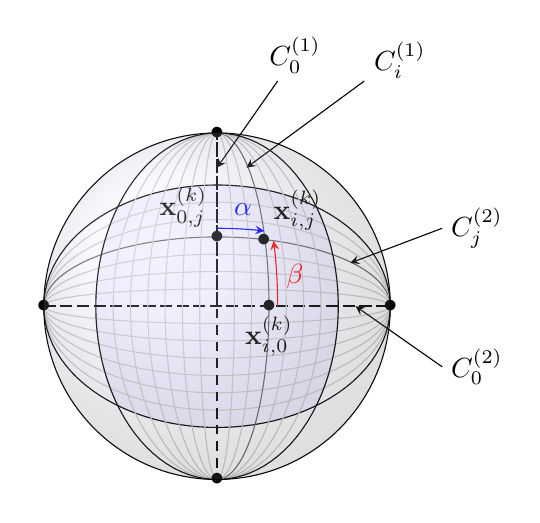
\begin{tikzpicture}[scale=2.2]
    \filldraw[draw=black,fill=blue!30!white,opacity=0.20]
	plot [smooth,domain=-35:35] ({0.7*cos(\x)},{sin(\x)})
	-- plot [smooth,domain=55:125] ({cos(\x)},{0.7*sin(\x)})
	-- plot [smooth,domain=140:215] ({0.7*cos(\x)},{sin(\x)})
	-- plot [smooth,domain=230:305] ({cos(\x)},{0.7*sin(\x)})
	-- cycle;	
	
	\draw [dashed, line width=0.8pt, samples=100,domain=180:-180] plot({cos(\x)},{0*sin(\x)});
	\draw [samples=100,domain=180:-180,color=gray!40] plot({cos(\x)},{0.1*sin(\x)});
	\draw [samples=100,domain=180:-180,color=gray!40] plot({cos(\x)},{0.2*sin(\x)});
	\draw [samples=100,domain=180:-180,color=gray!40] plot({cos(\x)},{0.3*sin(\x)});
	\draw [samples=100,domain=180:0,color=gray!120] plot({cos(\x)},{0.4*sin(\x)});
	\draw [samples=100,domain=0:-180,color=gray!40] plot({cos(\x)},{0.4*sin(\x)});
	\draw [samples=100,domain=180:-180,color=gray!40] plot({cos(\x)},{0.5*sin(\x)});
	\draw [samples=100,domain=180:-180,color=gray!40] plot({cos(\x)},{0.6*sin(\x)});
	\draw [samples=100,domain=180:-180] plot({cos(\x)},{0.7*sin(\x)});
	\draw [dashed, line width=0.8pt, samples=100,domain=180:-180] plot({0*cos(\x)},{sin(\x)});
	\draw [samples=100,domain=180:-180,color=gray!40] plot({0.1*cos(\x)},{sin(\x)});
	\draw [samples=100,domain=180:-180,color=gray!40] plot({0.2*cos(\x)},{sin(\x)});
	\draw [samples=100,domain=-90:90,color=gray!120] plot({0.3*cos(\x)},{sin(\x)});
	\draw [samples=100,domain=90:270,color=gray!40] plot({0.3*cos(\x)},{sin(\x)});
	\draw [samples=100,domain=180:-180,color=gray!40] plot({0.4*cos(\x)},{sin(\x)});
	\draw [samples=100,domain=180:-180,color=gray!40] plot({0.5*cos(\x)},{sin(\x)});
	\draw [samples=100,domain=180:-180,color=gray!40] plot({0.6*cos(\x)},{sin(\x)});
	\draw [samples=100,domain=180:-180] plot({0.7*cos(\x)},{sin(\x)}); 
	
	\draw [>=stealth, ->] (1.3,-.35) -- (.8,-0) ;
	\draw  (1.5,-.35) node {$C_0^{(2)}$} ;
	\draw [>=stealth, ->] (.35,1.3) -- (0,0.8) ;
	\draw  (.45,1.45) node {$C_0^{(1)}$} ;
	
	\draw [>=stealth, ->] (1.3,.45) -- (.77,0.25) ;
	\draw  (1.5,.45) node {$C_j^{(2)}$} ;
	
	\draw [>=stealth, ->] (.85,1.3) -- (.17,0.8) ;
	\draw  (.85,1.26) node[above right] {$C_i^{(1)}$} ;
	
	\draw  (0,1) node {$\bullet$} ;
	\draw  (0,-1) node {$\bullet$} ;
	\draw  (1,0) node {$\bullet$} ;
	\draw  (-1,0) node {$\bullet$} ;
	
	\draw  (.27,0.38) node {$\bullet$} ;
	\draw  (.27,0.38) node[above right] {$\mathbf{x}_{i,j}^{(k)}$} ;
	\draw  (0,0.4) node {$\bullet$} ;
	\draw  (0,0.4) node[above left] {$\mathbf{x}_{0,j}^{(k)}$} ;
	\draw  (0.3,0) node {$\bullet$} ;
	\draw  (.3,0) node[below] {$\mathbf{x}_{i,0}^{(k)}$} ;
	
	\draw [>=stealth, ->,samples=100,domain=90:75,color=blue] plot({1.05*cos(\x)},{0.45*sin(\x)});
	\draw  (.15,.65) node[color=blue, below] {$\alpha$} ;
	
	\draw [>=stealth, ->,samples=100,domain=0:21,color=red] plot({.35*cos(\x)},{1.05*sin(\x)});
	\draw  (.45,.3) node[color=red, below] {$\beta$} ;

	\draw (0,0) circle (1cm);
    \shade[ball color=blue!10!white,opacity=0.20] (0,0) circle (1cm);  
   
\end{tikzpicture}
\end{center}
\caption{Angles géodésiques $\alpha$ et $\beta$ pour le point $x_{i,j}^{(k)}$.}
\label{fig: alpha beta}
\end{figure}



\begin{figure}
\begin{center}
\begin{tikzpicture}[scale=2.5]
	\draw (1,3) -- (2,3) ; 
	\draw (0,2) -- (4,2) ; 	
	\draw (0,1) -- (4,1) ; 
	\draw (1,0) -- (2,0) ; 
	
	\draw (0,2) -- (0,1) ;
	\draw (1,3) -- (1,0) ;
	\draw (2,3) -- (2,0) ;
	\draw (3,2) -- (3,1) ;
	\draw (4,2) -- (4,1) ; 
	
	\draw [>=stealth, ->] (0.2,1.2) -- (0.5,1.2) ; 
	\draw (0.55,1.2) node[above]{$\alpha$} ; 
	\draw [>=stealth, ->] (0.2,1.2) -- (0.2,1.5) ; 
	\draw (0.3,1.4) node[above]{$\beta$} ; 
	\draw (0.7,1.7) node[above]{$(IV)$} ; 
	
	\draw [>=stealth, ->] (1.2,1.2) -- (1.5,1.2) ; 
	\draw (1.55,1.2) node[above]{$\alpha$} ; 
	\draw [>=stealth, ->] (1.2,1.2) -- (1.2,1.5) ; 
	\draw (1.3,1.4) node[above]{$\beta$} ; 
	\draw (1.7,1.7) node[above]{$(I)$} ; 
	
	\draw [>=stealth, ->] (2.2,1.2) -- (2.5,1.2) ; 
	\draw (2.55,1.2) node[above]{$\alpha$} ; 
	\draw [>=stealth, ->] (2.2,1.2) -- (2.2,1.5) ; 
	\draw (2.3,1.4) node[above]{$\beta$} ; 
	\draw (2.7,1.7) node[above]{$(II)$} ;
	
	\draw [>=stealth, ->] (3.2,1.2) -- (3.5,1.2) ; 
	\draw (3.55,1.2) node[above]{$\alpha$} ; 
	\draw [>=stealth, ->] (3.2,1.2) -- (3.2,1.5) ; 
	\draw (3.3,1.4) node[above]{$\beta$} ; 
	\draw (3.7,1.7) node[above]{$(III)$} ;  
	
	\draw [>=stealth, ->] (1.2,2.2) -- (1.5,2.2) ; 
	\draw (1.55,2.2) node[above]{$\alpha$} ; 
	\draw [>=stealth, ->] (1.2,2.2) -- (1.2,2.5) ; 
	\draw (1.3,2.4) node[above]{$\beta$} ; 
	\draw (1.7,2.7) node[above]{$(V)$} ; 
	
	\draw [>=stealth, ->] (1.2,0.2) -- (1.5,0.2) ; 
	\draw (1.55,0.2) node[above]{$\alpha$} ; 
	\draw [>=stealth, ->] (1.2,0.2) -- (1.2,0.5) ; 
	\draw (1.3,0.4) node[above]{$\beta$} ; 
	\draw (1.7,0.7) node[above]{$(VI)$} ; 
	
\end{tikzpicture}
\caption{Patron de la Cubed-Sphere avec orientation des directions $\alpha$ et $\beta$ par panel.}
\label{fig:patron cs}
\end{center}
\end{figure}

Soit $\mathbf{x}_{i,j}^{(I)}$ un point du panel $(I)$ de coordonnées $(x,y,z)$ dans $\mathbb{R}^3$. Alors les relations suivantes sont vérifiées :
\begin{equation}
\left\lbrace
\begin{array}{rcccc}
x & = & a \cos \alpha \cos \eta & = & a \cos \beta \cos \xi \\
y & = & a \sin \alpha & = & a \cos \beta \sin \xi \\
z & = & a \cos \alpha \sin \eta & = & a \sin \beta. \\
\end{array}
\right.
\label{eq: panel I xyz xi eta alpha beta}
\end{equation}
Des relations similaires existent sur tous les panels (voir Table \ref{tab: x y z fct de xi eta alfa beta}).

\begin{table}[htbp]
\begin{center}
%\rotatebox{90}{
\begin{tabular}{|c|c|}
\hline
\textbf{Panel} & $(x,y,z)$ \textbf{fonction de} $(\alpha, \eta)$ \textbf{et de} $(\xi, \beta)$ \\

\hline
\hline
    & $x=a \cos \alpha \cos \eta  =  a \cos \beta \cos \xi$ \\ 
$(I)$ & $y=a \sin \alpha  =  a \cos \beta \sin \xi$ \\
    & $z=a \cos \alpha \sin \eta  =  a \sin \beta$ \\
\hline
\hline
      & $x=- a \sin \alpha  = - a \cos \beta \sin \xi$ \\ 
$(II)$  & $y=a \cos \alpha \cos \eta  =  a \cos \beta \cos \xi$ \\
      & $z=a \cos \alpha \sin \eta  =  a \sin \beta$ \\
\hline
\hline
      & $x=- a \cos \alpha \cos \eta = a \cos \beta \cos \xi$ \\ 
$(III)$ & $y=- a \sin \alpha = - a \cos \beta \sin \xi$ \\
      & $z=a \cos \alpha \sin \eta = a \sin \beta$ \\
\hline
\hline
      & $x=a \sin \alpha = a \cos \beta \sin \xi$ \\ 
$(IV)$  & $y=- a \cos \alpha \cos \eta = - a \cos \beta \cos \xi$ \\
      & $z=a \cos \alpha \sin \eta = a \sin \beta$ \\
\hline
\hline
    & $x=-a \cos \alpha \sin \eta = - a \sin \beta$ \\ 
$(V)$ & $y=a \sin \alpha = a \cos \beta \sin \xi$ \\
    & $z=a \cos \alpha \cos \eta = a \cos \beta \cos \xi$ \\
\hline
\hline
     & $x=a \cos \alpha \sin \eta = a \sin \beta$ \\ 
$(VI)$ & $y=a \sin \alpha = a \cos \beta \sin \xi$ \\
     & $z=- a \cos \alpha \cos \eta = - a \cos \beta \cos \xi$ \\
\hline
\end{tabular}
%}
\end{center}
\caption{Coordonnées cartésiennes $(x,y,z)$ en fonction des angles $(\alpha, \eta)$ et de $(\xi, \beta)$  sur chaque panel.}
\label{tab: x y z fct de xi eta alfa beta}
\end{table}
Pour chaque panel, on peut déduire de \eqref{eq: panel I xyz xi eta alpha beta} les expressions de $\alpha$ et $\beta$ en fonction de $\xi$ et $\eta$. 

\begin{theoreme}
Les systèmes $(\alpha, \eta)$ et $(\xi, \beta)$ sont des systèmes de coordonnées admissibles sur chaque panel.
\end{theoreme} 

\begin{proof}
Sur le panel $(I)$ (d'après l'équation \eqref{eq: panel I xyz xi eta alpha beta} et le tableau \ref{tab: x y z fct de xi eta alfa beta}), on a :
\begin{equation}
\left\lbrace
\begin{array}{rcl}
x & = & a \cos \alpha \cos \eta \\
y & = & a \sin \alpha \\
z & = & a \cos \alpha \sin \eta
\end{array}
\right.
\label{eq:alfaeta_to_xyz}
\end{equation}
Or $x \neq 0$ sur le panel $(I)$ donc
\begin{eqsys}
\tan \eta = \frac{z}{x} \\
\sin \alpha = \frac{y}{a}
\label{eq:xyz_to_alfaeta}
\end{eqsys}
et par construction de la Cubed-Sphere, $\eta \in [- \pi/4, \pi/4]$ et $\alpha \in I \subset[- \pi/4, \pi/4]$. L'application
\begin{equation}
\varphi : (\alpha, \eta) \in \left[ - \dfrac{\pi}{4}, \dfrac{\pi}{4} \right]^2 \mapsto (x,y,z) \in \mathbb{R}^3
\end{equation}
donnée par \eqref{eq:alfaeta_to_xyz} est injective. La réciproque $\varphi^{-1} : (x,y,z) \in \Im(\varphi) \mapsto (\alpha, \eta) \in \left[ - \dfrac{\pi}{4}, \dfrac{\pi}{4} \right]^2$ est, d'après \eqref{eq:xyz_to_alfaeta}, donnée par $\alpha = \arcsin (y/a)$ et $\eta = \arctan(z/x)$ car $\sin$ et $\tan$ sont des bijections sur $\left[ - \dfrac{\pi}{4}, \dfrac{\pi}{4} \right]$. Comme $(x,y,z)$ est un système de coordonnées admissible sur le panel $(I)$ alors $(\alpha, \eta)$ en est un aussi. De plus, on a le même type de relations sur les autres panels.

La démonstration est la même pour montrer que $(\xi, \beta)$ est un système de coordonnées admissible par panel.
\end{proof}


\begin{proposition}
Les angles $\alpha$ et $\beta$ s'expriment en fonction des angles $\xi$ et $\eta$ par
\begin{eqsys}
\alpha(\xi, \eta) = \arctan \left[ \dfrac{\tan \xi}{\sqrt{1+\tan^2 \eta}} \right] \\
\beta(\xi,\eta) = \arctan \left[ \dfrac{\tan \eta}{\sqrt{1+\tan^2 \xi}} \right] .
\label{eq: alpha et beta fct de xi et eta}
\end{eqsys}
\label{prop:alfa_beta_xi_eta}
\end{proposition}

\begin{proof}
D'après l'équation \eqref{eq:alfaeta_to_xyz}, on a
\begin{equation}
x^2 + y^2 = a^2 \cos^2 \beta,
\end{equation}
ainsi que
\begin{equation}
z^2 = a^2 \sin^2 \beta,
\end{equation}
d'où on déduit facilement :
\begin{align*}
\tan^2 \beta & = \dfrac{z^2}{x^2+y^2} \\
	& = \dfrac{Y^2}{1+X^2}.
\end{align*}
L'expression de $\beta$ suivante se déduit
\begin{equation}
\beta(\xi, \eta) = \arctan \left[ \dfrac{\tan \eta}{\sqrt{1+\tan^2 \xi}} \right].
\end{equation}
De la même manière on obtient :
\begin{equation}
\alpha(\xi, \eta) = \arctan \left[ \dfrac{\tan \xi}{\sqrt{1+\tan^2 \eta}} \right].
\end{equation}
De plus, ces équations se retrouvent sur chaque panel.
\end{proof}


\begin{theoreme}
Les angles $(\alpha, \beta)$ forment un système de coordonnées admissible par panel.
\end{theoreme}

\begin{proof}
On définit l'application $\varphi$ permettant de passer des coordonnées gnomoniques $(X,Y) = (\tan \xi, \tan \eta)$ à $(\alpha,\beta)$. Cette application est donnée par
\begin{equation}
\varphi : \left\lbrace
\begin{array}{rcl}
[-1,1]^2 & \rightarrow & \Im (\varphi) \\
(X,Y) & \mapsto & (\alpha(X,Y), \beta(X,Y))
\end{array}
\right.
\end{equation}
avec $\alpha(X,Y)$ et $\beta(X,Y)$ vérifiant :
\begin{equation}
\alpha(X,Y) = \arctan \left[ \dfrac{X}{\sqrt{1+Y^2}} \right] \text{, et }
\beta(X,Y) = \arctan \left[ \dfrac{Y}{\sqrt{1+X^2}} \right].
\end{equation}
L'application $\varphi$ est continue, $[-1,1]^2$ est connexe donc $\Im (\varphi)$ est connexe. De plus, l'inclusion suivante est vérifiée :
\begin{equation}
\Im (\varphi ) \subset \left[ - \dfrac{\pi}{4}, \dfrac{\pi}{4}  \right]^2.
\end{equation}
L'application $\varphi$ est surjective par construction. Montrons qu'elle est injective. Supposons qu'il existe $(X_1,Y_1)$ et $(X_2,Y_2)$ dans $[-1,1]^2$ tels que 
\begin{equation}
\varphi(X_1,Y_1) = \varphi(X_2,Y_2).
\end{equation}
Comme $\arctan$ est bijective de $[-1,1]$ dans $[-\pi/4, \pi/4]$, cette relation est équivalente à
\begin{eqsys}
\dfrac{X_1}{\sqrt{1+Y_1^2}} = \dfrac{X_2}{\sqrt{1+Y_2^2}}\\
\dfrac{Y_1}{\sqrt{1+X_1^2}} = \dfrac{Y_2}{\sqrt{1+X_2^2}}.
\label{eq:sys1}
\end{eqsys} 
On pose $a = \dfrac{X_1}{\sqrt{1+Y_1^2}}$ et $b=\dfrac{Y_1}{\sqrt{1+X_1^2}}$. Le système \eqref{eq:sys1} implique :
\begin{eqsys}
X_2^2 - a^2 Y_2^2 = a^2 \\
-b^2 X_2^2 + Y_2^2 = b^2.
\label{eq:sys2}
\end{eqsys}
Le système \eqref{eq:sys2} est un système linéaire en $(X_2^2, Y_2^2)$. De plus, ce système est inversible, en effet pour que le système ne soit pas inversible, il faudrait que
\begin{align*}
0 & = \det \begin{bmatrix}
1 & - a^2 \\ -b^2 & 1
\end{bmatrix} \\
  & = 1 - a^2 b^2.
\end{align*}
En remplaçant $a$ et $b$ par leur valeur, cette dernière relation implique
\begin{equation}
0 = 1 + X_1^2 + Y_1^2,
\end{equation}
ce qui est impossible. Donc le système \eqref{eq:sys2} admet une unique solution et cette dernière est donnée par
\begin{eqsys}
X_2^2 = \dfrac{a^2(b^2 +1)}{1 - a^2 b^2} = X_1^2 \\
Y_2^2 = \dfrac{b^2(a^2 +1)}{1 - a^2 b^2} = Y_1^2.
\end{eqsys}
Donc on obtient $X_1 = \pm X_2$ et $Y_1 = \pm Y_2$. Or si $X_1 = - X_2$, on a
\begin{equation}
\dfrac{X_1}{\sqrt{1+Y_1^2}} = -\dfrac{X_1}{\sqrt{1+Y_2^2}},
\end{equation}
d'où on déduit directement
\begin{equation}
\sqrt{1+Y_1^2} = -\sqrt{1+Y_2^2},
\end{equation}
ce qui est absurde. Donc on ne peut pas avoir $X_1 = - X_2$. De la même manière, on ne peut pas avoir $Y_1 = - Y_2$. On en déduit que $(X_1,Y_1) = (X_2,Y_2)$ et l'application $\varphi$ est bijective.

Enfin on a vu que $(X,Y)$ est un système de coordonnées admissible par panel donc $(\alpha, \beta)$ est un système de coordonnées admissible par panel.
\end{proof}





















Chacune des sections de grand cercle peut être complétée en un grand cercle. Le grand cercle $C_i^{(1)}$ correspond à une isoligne $\xi$ constante et le grand cercle $C_j^{(2)}$ à une isoligne $\eta$ constante. Considérons l'isoligne $\eta$ constante sur le panel $(I)$. Sur ce panel, l'angle $\alpha$ est tel que :
\begin{equation}
- \alpha_0 (\eta) \leq \alpha \leq \alpha_0(\eta) \text{ avec } \alpha_0( \eta) = \arctan \left( \dfrac{\sqrt{2}}{2} \tan \eta \right).
\end{equation}
Le grand cercle $C_j^{(2)}$ traverse sur les panels $(II)$, $(III)$ et $(IV)$ dans cet ordre. On peut prolonger $\alpha$ comme étant l'angle curviligne le long du grand cercle complet. Sur le panel $(II)$, le grand cercle $C_j^{(2)}$ coupe d'autres grands cercles (ceux permettant de construire le panel $(II)$) en $\mathbf{M}_k$ ($-N/2 \leq k \leq N/2$) de coordonnées $(\xi^E_k = k \Delta \xi, \eta^E_k)$. Il coupe aussi le panel $(III)$ mais correspond aux points de maillage par symétrie, soit le grand cercle du panel $(III)$ correspondant à l'isoligne $\eta^B_k = \frac{\pi}{2} - \eta$. Enfin, le grand cercle $C_j^{(2)}$ traverse le panel $(IV)$ aux points de coordonnées $(\xi^W_k = k \Delta \xi, \eta^W_k)$. 

De la même manière, le grand cercle $C_i^{(1)}$ traverse les panels $(V)$, $(III)$ et $(VI)$ dans cet ordre et est paramétré par l'angle $\beta$.

Les autres panels $(II)$, $(III)$, $(IV)$, $(V)$, $(VI)$ sont traités de la même manière. Compte tenu des symétries de la Cubed-Sphere, six familles de grands cercles sont à considérer. On définit les familles de grands cercles suivants :

\begin{itemize}
\item $(I_{\alpha})$ et $(I_{\beta})$ sont les grands cercles passant par le panel $(I)$. Ils sont définis comme les isolignes en $\eta$ et en $\xi$ (du panel $(I)$) respectivement,
\item $(II_{\alpha})$ et $(II_{\beta})$ sont les grands cercles passant par le panel $(II)$. Ils sont définis comme les isolignes en $\eta$ et en $\xi$ (du panel $(II)$) respectivement,
\item $(V_{\alpha})$ et $(V_{\beta})$ sont les grands cercles passant par le panel $(V)$. Ils sont définis comme les isolignes en $\eta$ et en $\xi$ (du panel $(V)$) respectivement.
\end{itemize}

\begin{figure}
\begin{center}
\includegraphics[scale=0.3]{fig21.jpg}
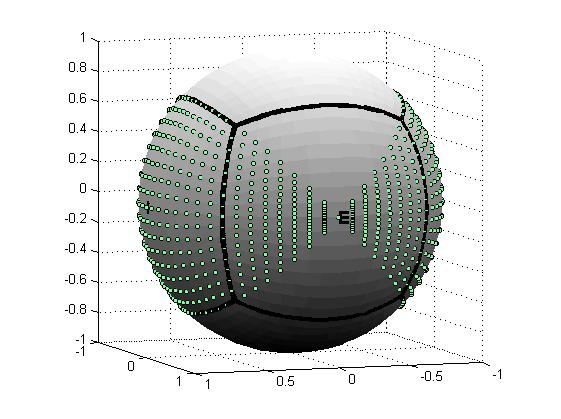
\includegraphics[scale=0.3]{fig22.jpg}
\end{center}
\caption{L'ensemble $(I_{\alpha})$ de grands cercles correspond aux isolignes $\eta$ constant du panel $(I)$ et du panel $(III)$.}
\end{figure}


La structure de la Cubed-Sphere décrite par des grands cercles est à la base du procédé de calcul des dérivées hermitiennes que nous utilisons dans ce travail. Le calcul du gradient suit la procédure suivante :
\begin{enumerate}
\item Construction de données le long de grands cercles complets,
\item Calcul des dérivées hermitiennes sur les grands cercles,
\item Assemblage pour obtenir le gradient.
\end{enumerate}

Pour calculer $\dfrac{\partial h}{\partial \alpha}_{|C_1}$ et $\dfrac{\partial h}{\partial \beta}_{|C_2}$ aux points de maillage, il est utile de connaître les coordonnées des points d'intersections de grands cercles entre les panels.

Soit $h_{i,j}^{(k)}$ donné avec $-N/2 \leq i,j \leq N/2$ et $(k) = (I), (II), (III), (IV), (V), (VI)$. Considérons le grand cercle $C_1 \in (I_{\alpha})$. Il correspond à l'isoligne $\eta = \eta_0^F = j_0 \Delta \eta$. Les valeurs $h_{i,j_0}^F$ sont localisée sur un grand cercle avec $-N/2 \leq i \leq N/2$. Le cercle $C_1$ traverse le panel $(II)$ sur lequel il faut interpoler les données pour compléter les valeurs le long de $C_1$ sur le panel $(II)$. Le cercle $C_1$ coupe chaque isoligne $\xi = \xi^E_{i_0} = i_0 \Delta \xi$ au point de coordonnées $(\xi_{i_0}^E, \beta_{i_0,j_0})$ dans le système de coordonnées $(\xi^E, \beta)$ du panel $(II)$. Un point $\mathbf{x}(x,y,z)\in \mathbb{R}^3$ d'un cercle de la famille $(II_{\beta})$ satisfait les relations :
\begin{equation}
\left\lbrace
\begin{array}{rcl}
x & = & - a \cos \beta \sin \xi^E \\
y & = & a \cos \beta \cos \xi^E \\
z & = & a \sin \beta.
\end{array}
\right.
\end{equation}
Le point $\mathbf{x}(x,y,z)$ se situe à l'intersection de $C_1$ (isocline $\eta^F_{j_0}$ du panel $(I)$) avec le grand cercle correspondant à l'isocline $\xi = \xi^E_{i_0} = i_0 \Delta \xi$. Alors $x$, $y$ et $z$ sont solutions du système suivant :

\begin{equation}
\left\lbrace
\begin{array}{rcccl}
x & = & a \cos \alpha_{i_0, j_0} \cos \eta^F_{j_0} & = & a \cos \beta_{i_0, j_0} \cos \xi^E_{i_0} \\
y & = & a \sin \alpha_{i_0, j_0} & = & a \cos \beta_{i_0, j_0} \cos \xi^E_{i_0} \\
z & = & a \cos \alpha_{i_0, j_0} \sin \eta^F_{j_0}  & = & a \sin \beta_{i_0, j_0}.
\end{array}
\right.
\end{equation}
De là, il découle :
\begin{equation}
\dfrac{z}{x} = \tan \eta^F_{j_0} = - \dfrac{\sin \beta_{i_0, j_0}}{\cos \beta_{i_0, j_0} \sin \xi^E_{i_0}}
\end{equation}
donc :
\begin{equation}
\beta_{i_0, j_0} = \arctan \left[ - \tan \eta^F_{j_0} \sin \xi^E_{i_0} \right].
\label{eq:coord_cross}
\end{equation}
Ainsi, le point du panel $(II)$ de coordonnées $(\xi, \beta)$, représentant l'intersection de l'isocline $\eta^F_{j_0}$ du panel $(I)$ avec l'isocline $\xi_{i_0}^E$ du panel $(II)$, est donné par $(\xi^E_{i_0}, \beta_{i_0, j_0})$. En général, il ne s'agit pas d'un point de la Cubed-Sphere. Nous utilisons une méthode de spline cubique pour obtenir des valeurs $u_{i_0,j}^{(II)}$ interpolées sur la totalité de $C$.
En continuant ce procédé, nous obtenons des valeurs sur le cercle $C$.







On calcule à présent les dérivées partielles $\dfrac{\partial h}{\partial \alpha}_{|C_1}$ et $\dfrac{\partial h}{\partial \beta}_{|C_2}$ en fonction des paramètres $\xi$ et $\eta$. Par composition, les relations suivantes sont vérifiées :
\begin{equation}
\begin{array}{rcl}
\dfrac{\partial h}{\partial \alpha}_{|C_1} & = &  \dfrac{1}{\frac{\partial \alpha}{\partial \xi}_{|C_1}} \dfrac{\partial h}{\partial \xi}_{|C_1} \\
\dfrac{\partial h}{\partial \beta}_{|C_2} & = &  \dfrac{1}{\frac{\partial \beta}{\partial \eta}_{|C_2}} \dfrac{\partial h}{\partial \eta}_{|C_2} \\
\end{array}
\label{eq: derivee partiel link}
\end{equation}
car $\eta \mapsto \alpha$ est constant le long de $C_2 \in (I_{\alpha})$ et $\xi \mapsto \beta$ est constant le long de $C_1 \in (I_{\beta})$. 






On calcule les vecteurs $\mathbf{g}_{\alpha}$, $\mathbf{g}_{\beta}$, $\mathbf{g}^{\alpha}$ et $\mathbf{g}^{\beta}$ en fonction de $\mathbf{g}_{\xi}$, $\mathbf{g}_{\eta}$, $\mathbf{g}^{\xi}$ et $\mathbf{g}^{\eta}$ :

\begin{proposition}
Les expressions suivantes sont vérifiées :
\begin{itemize}
\item $\mathbf{e}_{\alpha} = \dfrac{1}{\frac{\partial \alpha}{\partial \xi}_{|C_1}} \mathbf{g}_{\xi}$ le long de $C_1$,
\item $\mathbf{e}_{\beta} = \dfrac{1}{\frac{\partial \beta}{\partial \eta}_{|C_2}} \mathbf{g}_{\eta}$ le long de $C_2$,
\item $\mathbf{e}^{\alpha} = \dfrac{\partial \alpha}{\partial \xi}_{|C_1} \mathbf{g}^{\xi}$ le long de $C_1$,
\item $\mathbf{e}^{\beta} = \dfrac{\partial \beta}{\partial \eta}_{|C_2} \mathbf{g}^{\eta}$ le long de $C_2$.
\end{itemize}
\label{prop: g_alpha g_beta fct de g_xi g_eta}
\end{proposition}

\begin{proof}
\begin{itemize}
\item Par définition et composition, le long de $C_1$, on a :
\begin{align*}
\mathbf{g}_{\xi} & = \dfrac{d \mathbf{x}}{d \xi}_{|\eta}\\
	& = \dfrac{\partial \alpha}{\partial \xi}_{|\eta} \dfrac{\partial \mathbf{x}}{\partial \alpha}_{|\eta} + \dfrac{\partial \beta}{\partial \xi}_{|\eta} \dfrac{\partial \mathbf{x}}{\partial \beta}_{|\eta}\\
	& = \dfrac{\partial \alpha}{\partial \xi}_{|\eta} \dfrac{\partial \mathbf{x}}{\partial \alpha}_{|\eta}.
\end{align*}
De cette dernière relation, il découle la première égalité :
\begin{equation}
\mathbf{e}_{\alpha} = \dfrac{1}{\frac{\partial \alpha}{\partial \xi}_{|\eta}} \mathbf{g}_{\xi}.
\end{equation}
De la même manière :
\begin{equation}
\mathbf{e}_{\beta} = \dfrac{1}{\frac{\partial \beta}{\partial \eta}_{|\xi}} \mathbf{g}_{\eta}.
\end{equation}

\item On pose $\mathbf{u} = \dfrac{\partial \alpha}{\partial \xi}_{|\eta} \mathbf{g}^{\xi}$ et $\mathbf{v} = \dfrac{\partial \beta}{\partial \eta}_{|\xi} \mathbf{g}^{\eta}$. Donc le long de $C_1$, on a:
\begin{equation}
\mathbf{e}_{\alpha} \cdot \mathbf{u} = \dfrac{\frac{\partial \alpha}{\partial \xi}_{|\eta}}{\frac{\partial \alpha}{\partial \xi}_{|\eta}} \mathbf{g}_{\xi} \cdot \mathbf{g}^{\xi} = 1.
\end{equation}
De plus :
\begin{equation}
\mathbf{e}_{\beta} \cdot \mathbf{u} = \dfrac{\frac{\partial \alpha}{\partial \xi}_{|\eta}}{\frac{\partial \beta}{\partial \eta}_{|\xi}} \mathbf{g}_{\eta} \cdot \mathbf{g}^{\xi} = 0
\end{equation}
Donc $\mathbf{e}^{\alpha} = \mathbf{u}$. De la même manière, on montre que $\mathbf{e}^{\beta} = \mathbf{v}$ le long de $C_2$.
\end{itemize}
\end{proof}




\begin{theoreme}
Soit $h : \mathbb{S}_a^2 \rightarrow \mathbb{R}$ une fonction régulière. Alors :
\begin{equation}
\nabla_T h = \dfrac{\partial h}{\partial \xi}_{|\eta = \bar{\eta}} \mathbf{g}^{\xi} + \dfrac{\partial h}{\partial \eta}_{|\xi = \bar{\xi}} \mathbf{g}^{\eta}.
\end{equation}
\label{th:gradient_xieta}
\end{theoreme}


\begin{proof}
Les égalités suivantes sont vérifiées grâce à la proposition \ref{prop: g_alpha g_beta fct de g_xi g_eta} et aux équations \eqref{eq: derivee partiel link} :
\begin{equation}
\dfrac{\partial h}{\partial \alpha}_{|C_1} \mathbf{e}^{\alpha} = \dfrac{1}{\alpha'(\xi)} \dfrac{\partial h}{\partial \xi}_{|\eta = \bar{\eta}} \alpha'(\xi) \mathbf{g}^{\xi} = \dfrac{\partial h}{\partial \xi}_{|\eta = \bar{\eta}} \mathbf{g}^{\xi}
\end{equation}
De même on a:
\begin{equation}
\dfrac{\partial h}{\partial \beta}_{|C_2} \mathbf{e}^{\beta} =  \dfrac{\partial h}{\partial \eta}_{|\xi = \bar{\xi}} \mathbf{g}^{\eta}
\end{equation}
d'où le résultat à l'aide de la formule \eqref{eq: gradient}.
\end{proof}































\section{Harmoniques Sphériques sur la Cubed-Sphere}

Pour résoudre des problèmes sur la sphère, les harmoniques sphériques jouent un rôle particulièrement important \cite{Atkinson2012, Frye2012}. On les utilise pour décomposer des fonctions de carré intégrable. On note $\mathbf{Y}^l_m$ les harmoniques sphériques avec $l \in \mathbb{N}$ et $|m| \leq l$, $m \in \mathbb{Z}$. Les harmoniques sphériques sur $\mathbb{S}_a^2$ s'expriment en fonction de $(\lambda, \theta)$, les coordonnées longitude-latitude, par
\begin{equation}
\mathbf{Y}_m^l(\mathbf{x}) = \mathbf{Y}_m^l(\lambda, \theta) = \dfrac{(-1)^m}{a} \sqrt{\dfrac{(2l+1)}{4 \pi} \dfrac{(l-|m|)!}{(l+|m|)!}} P^{|m|}_l (\sin (\theta)) \exp \left( i m \lambda \right),
\label{eq:harmoniques_spheriques}
\end{equation}
où $P^m_l$ désignent les polynômes de Legendre associés \cite{Atkinson2012, Lagrange1939}. Ils s'expriment grâce à la formule
\begin{equation}
P^m_l(x) = \dfrac{1}{2^l l!}(1-x^2)^{m/2} \dfrac{d^l}{dx^l} \left( (x^2-1)^l \right).
\end{equation}
En particulier, on a 
\begin{equation}
\mathbf{Y}_0^0(\mathbf{x}) = \dfrac{1}{a \sqrt{4 \pi}}.
\end{equation}

Toute fonction $f : \mathbf{x} \in \mathbb{S}_a^2 \mapsto f(\mathbf{x})$ de carré intégrable s'écrit comme combinaison linéaire des harmoniques sphériques. Autrement dit, il existe une famille $(f_{m,l})_{l \in \mathbb{N}, |m| \leq l}$ de $\mathbb{C}$ telle que
\begin{equation}
f = \gsum_{l \in \mathbb{N}} \gsum_{m= -l}^l f_{m,l} \mathbf{Y}^l_m.
\end{equation}
Les harmoniques sphériques $\mathbf{Y}^l_m$ forment une famille orthonormée de $L^2(\mathbb{S}^2_a)$ \cite{Atkinson2012}, c'est à dire
\begin{equation}
\gint_{\mathbb{S}_a^2} \mathbf{Y}^l_m(\mathbf{x}) \bar{\mathbf{Y}}^{l'}_{m'}(\mathbf{x}) d \sigma (\mathbf{x}) = \delta_{m, m'}\delta_{l, l'}
\label{eq:HS_perp}
\end{equation}
où $\delta_{p,q}$ désigne le symbole de Kronecker de $p$ et $q$.

Dans cette partie, on s'intéresse à la version discrète sur la Cubed-Sphere de ces résultats. Pour cela nous définissons un produit scalaire pondéré sur le maillage et analysons la version discrète de l'équation \eqref{eq:HS_perp}. La conception et l'étude d'un produit scalaire sur la Cubed-Sphere sont liées à la conception d'une méthode de quadrature. Une étude a déjà été réalisée dans \cite{Portelenelle2018} dans le cadre de méthodes permettant d'approcher l'intégrale.











\subsection{Produit scalaire discret sur la Cubed-Sphere}

Sur un panel $(k) = (I), \cdots , (VI)$ donné, on note $I^{(k)}(f)$ l'intégrale d'une fonction $f : \mathbf{x} \in \mathbb{S}_a^2 \mapsto f(\mathbf{x}) \in \mathbb{C}$ (supposée intégrable) :
\begin{equation}
I^{(k)}(f) = \gint_{(k)}f(\mathbf{x}) d\sigma(\mathbf{x}).
\end{equation}

\begin{proposition}
Soit  $f : \mathbf{x} \in \mathbb{S}_a^2 \mapsto f(\mathbf{x}) \in \mathbb{C}$ une fonction intégrable sur la sphère $\mathbb{S}_a^2$. Alors pour tout panel $(k)=(I), \cdots, (VI)$, nous avons
\begin{equation}
I^{(k)} = \gint_{[-\pi/4, \pi/4]^2} f(\xi, \eta) \sqrt{\det (\mathbf{G})} d\xi d\eta.
\end{equation}
où $(\xi, \eta)$ sont les coordonnées d'un point du panel définies dans la section \ref{sec:gnomonique}.
\end{proposition}

\begin{proof}
On définit $\psi_{(k)}$ l'application permettant de passer des coordonnées $(\xi, \eta)$ associées au panel $(k)$ aux coordonnées cartésiennes . L'application $\psi_{(k)}$ est bien définie car $(\xi, \eta)$ est un système de coordonnées admissibles sur le panel $(k)$. On a
\begin{equation}
\psi_{(k)} : (\xi, \eta) \in \left[ - \dfrac{\pi}{4}, \dfrac{\pi}{4} \right]^2 \mapsto \mathbf{x}(\xi, \eta) \in (k).
\end{equation}
Par exemple, sur le panel $(I)$ on a :
\begin{equation}
\psi_{(I)} : (\xi, \eta) \in \left[ - \dfrac{\pi}{4}, \dfrac{\pi}{4} \right]^2 \mapsto \mathbf{x}(\xi, \eta) = (x,y,z) \in (I) \subset \mathbb{R}^3,
\end{equation}
or les relations suivantes sont vérifiées :
\begin{eqsys}
X= \tan \xi = \dfrac{y}{x} \\
Y= \tan \eta = \dfrac{z}{x} \\
a^2 = x^2+y^2+z^2.
\end{eqsys}
Donc $\mathbf{x}(x,y,z)$ est donné par
\begin{equation}
\left\lbrace
\begin{array}{rcl}
x & = & \dfrac{a}{\sqrt{1 + \tan^2 (\xi) + \tan^2 (\eta)}} \\
y & = & \dfrac{a \tan (\xi)}{\sqrt{1 + \tan^2 (\xi) + \tan^2 (\eta)}} \\
z & = & \dfrac{a \tan ( \eta )}{\sqrt{1 + \tan^2 (\xi) + \tan^2 (\eta)}}.
\end{array}
\right.
\end{equation}
Des relations similaires peuvent être déduites sur tous les panels. 
\begin{align*}
\gint_{(k)} f(\mathbf{x}) d \sigma(\mathbf{x}) & = \gint_{[-\pi/4, \pi/4]^2} f_k(\psi_{(k)}(\xi, \eta)) |\det J_{\psi_{(k)}}(\xi, \eta)| d\xi d\eta \\
	&  = \gint_{[-\pi/4, \pi/4]^2} f(\psi_{(k)}(\xi, \eta)) \sqrt{\det (\mathbf{G})} d\xi d\eta \\
\end{align*}
avec $J_{\psi_{(k)}}$ la matrice Jacobienne de $\psi_{(k)}$. En notant $f_k = f \circ \psi_{(k)}$, on a
\begin{equation}
I^{(k)} = \gint_{[-\pi/4, \pi/4]^2} f_k(\xi, \eta) \sqrt{\det (\mathbf{G})} d\xi d\eta.
\end{equation}
\end{proof}

Les panels $(I), \cdots, (VI)$ couvrent la totalité de la Cubed-Sphere et sont disjoints. Donc en notant
\begin{equation}
I(f) = \gint_{\mathbb{S}_a^2}f(\mathbf{x}) d \sigma(\mathbf{x}),
\end{equation}
on obtient la relation
\begin{equation}
I(f) = \gsum_{(k)=(I)}^{(VI)} I^{(k)}(f).
\end{equation}
Par analogie avec l'intégrale, nous nous intéressons à des produits scalaires de la forme
\begin{equation}
<\bu, \bv>_{\CS} = \gsum_{(k)=(I)}^{(VI)} \left( \Delta \xi \Delta \eta \gsum_{i=-N/2}^{N/2} \gsum_{j=-N/2}^{N/2} \omega_{i,j} \bu_{i,j}^{(k)} \bar{\bv}_{i,j}^{(k)} \sqrt{\bar{\mathbf{G}}_{i,j}} \right)
\end{equation}
où $\bu$ et $\bv$ sont des fonctions de grille sur la Cubed-Sphere. De plus, nous notons $\bar{\mathbf{G}}_{i,j} = \det (\mathbf{G}(\xi_i, \eta_j))$. Pour tout $-N/2 \leq i,j \leq N/2$, on note $\omega_{i,j}>0$ un poids donné.

\begin{proposition}
$<\cdot, \cdot>_{\CS}$ définit un produit scalaire hermitien sur l'espace des fonctions de grille sur la Cubed-Sphere.
\end{proposition}















\subsection{Harmoniques sphériques sur la Cubed-Sphere}

Pour les produits scalaires de la forme $<\cdot, \cdot>_{\CS}$, on analyse l'orthogonalité des harmoniques sphériques restreintes au maillages. Pour cela, on commence par observer les propriétés de symétrie suivantes :

\begin{lemme}
Soit $l \in \mathbb{N}$ et $m$ tel que $|m| \leq l$. Alors à tout harmonique sphérique $\mathbf{Y}_m^l$, si $(\lambda, \theta) \in ]0,2 \pi] \times ]-\pi/2, \pi/2[$ représente les coordonnées longitude-latitude, on a les relations de symétrie suivantes :
\begin{itemize}
\item $\mathbf{Y}^l_m (\lambda, \theta) = (-1)^{m+l} \mathbf{Y}^l_m (\lambda, -\theta)$,
\item $\mathbf{Y}^l_m (\lambda + \alpha, \theta) = e^{i m \alpha} \mathbf{Y}^l_m \left(\lambda, \theta \right)$,
\item $\mathbf{Y}^l_m (\lambda, \theta) = \bar{\mathbf{Y}}^l_m (-\lambda, \theta)$.
\end{itemize}
\label{lem:HS_sym}
\end{lemme}

En tenant compte de ces symétries sur les harmoniques sphériques, il suffit d'ajouter des symétries semblables aux poids $\omega_{i,j}$ dans la définition du produit scalaire $<\cdot, \cdot>_{\CS}$ pour que des compensations apparaissent entre les panels de la Cubed-Sphere. On a le résultat suivant :

\begin{theoreme}
Soient $\mathbf{Y}_m^{l}$ et $\mathbf{Y}_{m'}^{l'}$ deux harmoniques sphériques avec $l, l' \in \mathbb{N}$, $|m| \leq l$ et $|m'| \leq l'$. On suppose que pour tout $-N/2 \leq i,j \leq N/2$, les poids $(\omega_{i,j})_{-N/2 \leq i,j \leq N/2}$ satisfont
\begin{equation}
\omega_{i,j} = \omega_{-i,j} = \omega_{-i,-j} = \omega_{i,-j}>0
\label{eq:sym_omega}
\end{equation}
alors les fonctions de grilles restreintes à la Cubed-Sphere $\mathbf{Y}_m^{l,*}$ et $\mathbf{Y}_{m'}^{l',*}$ satisfont
\begin{equation}
<\mathbf{Y}_{m}^{l,*},\mathbf{Y}_{m'}^{l',*}>_{\CS} = 0 
\end{equation}
si $m+m'$ ou $l+l'$ est impair.
En particulier on a
\begin{equation}
<\mathbf{Y}_{m}^{l,*},\mathbf{Y}_{0}^{0,*}>_{\CS} = 0 
\end{equation}
lorsque
\begin{itemize}
\item $m$ impair ou bien,
\item $l$ impair ou bien,
\item $l$ pair et $m \equiv 2 [4]$.
\end{itemize}
\label{th:pdtscal_HS}
\end{theoreme}

\begin{proof}
Soit $(k) = (I) , \cdots, (VI)$. Nous adoptons la notation
\begin{equation}
S_{(k)} = \Delta \xi \Delta \eta \gsum_{i=-N/2}^{N/2} \gsum_{j=-N/2}^{N/2} \omega_{i,j} (\mathbf{Y}_m^{l,*})_{i,j}^{(k)} (\bar{\mathbf{Y}}_{m'}^{l',*})_{i,j}^{(k)} \sqrt{\bar{\mathbf{G}}_{i,j}}.
\end{equation}
Donc la relation suivante est vérifiée :
\begin{equation}
S = <\mathbf{Y}_{m}^{l,*},\mathbf{Y}_{m'}^{l',*}>_{\CS} = \gsum_{(k)=(I)}^{(VI)} S_{(k)}.
\end{equation}
D'après les relations de symétrie sur $\omega_{i,j}$ \eqref{eq:sym_omega} et sur les harmoniques sphériques (lemme \ref{lem:HS_sym}), on a
\begin{align*}
S_{(I)} & = \Delta \xi \Delta \eta \gsum_{i=-N/2}^{N/2} \gsum_{j=-N/2}^{N/2} \omega_{i,j} (\mathbf{Y}_m^{l,*})_{i,j}^{(I)} (\bar{\mathbf{Y}}_{m'}^{l',*})_{i,j}^{(I)} \sqrt{\bar{\mathbf{G}}_{i,j}} \\
	& = (-1)^{l+l'} \Delta \xi \Delta \eta \gsum_{i=-N/2}^{N/2} \gsum_{j=-N/2}^{N/2} \omega_{i,j} (\mathbf{Y}_m^{l,*})_{i,j}^{(III)} (\bar{\mathbf{Y}}_{m'}^{l',*})_{i,j}^{(III)} \sqrt{\bar{\mathbf{G}}_{i,j}} \\
	& = (-1)^{l+l'}S_{(III)}.
\end{align*}
De la même manière, on a
\begin{equation}
S_{(II)} = (-1)^{l+l'}S_{(IV)}.
\label{proof:symII_IV}
\end{equation}
Les panels $(V)$ et $(VI)$ étant symétriques par rapport à l'équateur, en utilisant le premier point du lemme \ref{lem:HS_sym}, on a
\begin{equation}
S_{(V)} = (-1)^{m+m'+l+l'} S_{(VI)}.
\label{proof:symV_VI}
\end{equation}
En combinant \eqref{proof:symII_IV} et \eqref{proof:symV_VI}, on montre que
\begin{equation}
S=(1+(-1)^{l+l'})(S_{(I)} + S_{(II)}) + (1+(-1)^{l+l'+m+m'})S_{(V)}.
\end{equation}
Les points du panel $(I)$ se déduisent par rotation d'angle $\pi/2$ à partir de ceux du panel $(II)$. De plus, d'après le lemme \ref{lem:HS_sym}, on a
\begin{equation}
\mathbf{Y}^{l}_m(\lambda + \pi/2, \theta) = \exp \left( - i m \dfrac{\pi}{2}  \right) \mathbf{Y}^{l}_m(\lambda, \theta).
\end{equation}
Partant de ces relations entre les panels $(I)$ et $(II)$, on trouve
\begin{equation}
S = (1+(-1)^{l+l'})\left( \exp \left( -i(m+m') \dfrac{\pi}{2} \right) +1 \right)S_{(I)} + (1+(-1)^{l+l'+m+m'})S_{(V)}.
\end{equation}
Le problème est à présent de savoir si on peut avoir $S_{(I)}=0$ ou $S_{(V)} = 0$.

Considérons d'abord le panel $(I)$. On a
\begin{align*}
S_{(I)} & = \Delta \xi \Delta \eta \gsum_{i=-N/2}^{N/2} \gsum_{j=-N/2}^{N/2} \omega_{i,j} (\mathbf{Y}_m^{l,*})_{i,j}^{(I)} (\bar{\mathbf{Y}}_{m'}^{l',*})_{i,j}^{(I)} \sqrt{\bar{\mathbf{G}}_{i,j}} \\
	& = S_1 + S_2 + S_3 +S_4,
\end{align*}
avec $S_1$ donné par
\begin{align*}
S_1 = & \Delta \xi \Delta \eta \gsum_{i=-N/2}^{1} \gsum_{j=1}^{N/2} \omega_{i,j} (\mathbf{Y}_m^{l,*})_{i,j}^{(I)} (\bar{\mathbf{Y}}_{m'}^{l',*})_{i,j}^{(I)} \sqrt{\bar{\mathbf{G}}_{i,j}} \\
	& + \dfrac{\Delta \xi \Delta \eta}{2} \gsum_{i=-N/2}^{1} \omega_{i,0} (\mathbf{Y}_m^{l,*})_{i,0}^{(I)} (\bar{\mathbf{Y}}_{m'}^{l',*})_{i,0}^{(I)} \sqrt{\bar{\mathbf{G}}_{i,0}}\\
		& + \dfrac{\Delta \xi \Delta \eta}{2} \gsum_{j=1}^{N/2} \omega_{0,j} (\mathbf{Y}_m^{l,*})_{0,j}^{(I)} (\bar{\mathbf{Y}}_{m'}^{l',*})_{0,j}^{(I)} \sqrt{\bar{\mathbf{G}}_{0,j}}\\
		& + \dfrac{\Delta \xi \Delta \eta}{4} (\mathbf{Y}_m^{l,*})_{0,0}^{(I)} (\bar{\mathbf{Y}}_{m'}^{l',*})_{0,0}^{(I)} \sqrt{\bar{\mathbf{G}}_{0,0}},
\end{align*}
$S_2$ donné par
\begin{align*}
S_2 = & \Delta \xi \Delta \eta \gsum_{i=-N/2}^{1} \gsum_{j=-N/2}^{1} \omega_{i,j} (\mathbf{Y}_m^{l,*})_{i,j}^{(I)} (\bar{\mathbf{Y}}_{m'}^{l',*})_{i,j}^{(I)} \sqrt{\bar{\mathbf{G}}_{i,j}} \\
	& + \dfrac{\Delta \xi \Delta \eta}{2} \gsum_{i=-N/2}^{1} \omega_{i,0} (\mathbf{Y}_m^{l,*})_{i,0}^{(I)} (\bar{\mathbf{Y}}_{m'}^{l',*})_{i,0}^{(I)} \sqrt{\bar{\mathbf{G}}_{i,0}}\\
		& + \dfrac{\Delta \xi \Delta \eta}{2} \gsum_{j=-N/2}^{1} \omega_{0,j} (\mathbf{Y}_m^{l,*})_{0,j}^{(I)} (\bar{\mathbf{Y}}_{m'}^{l',*})_{0,j}^{(I)} \sqrt{\bar{\mathbf{G}}_{0,j}}\\
		& + \dfrac{\Delta \xi \Delta \eta}{4} (\mathbf{Y}_m^{l,*})_{0,0}^{(I)} (\bar{\mathbf{Y}}_{m'}^{l',*})_{0,0}^{(I)} \sqrt{\bar{\mathbf{G}}_{0,0}},
\end{align*}
$S_3$ donné par
\begin{align*}
S_3 = & \Delta \xi \Delta \eta \gsum_{i=1}^{N/2} \gsum_{j=-N/2}^{1} \omega_{i,j} (\mathbf{Y}_m^{l,*})_{i,j}^{(I)} (\bar{\mathbf{Y}}_{m'}^{l',*})_{i,j}^{(I)} \sqrt{\bar{\mathbf{G}}_{i,j}} \\
	& + \dfrac{\Delta \xi \Delta \eta}{2} \gsum_{i=1}^{N/2} \omega_{i,0} (\mathbf{Y}_m^{l,*})_{i,0}^{(I)} (\bar{\mathbf{Y}}_{m'}^{l',*})_{i,0}^{(I)} \sqrt{\bar{\mathbf{G}}_{i,0}}\\
		& + \dfrac{\Delta \xi \Delta \eta}{2} \gsum_{j=-N/2}^{1} \omega_{0,j} (\mathbf{Y}_m^{l,*})_{0,j}^{(I)} (\bar{\mathbf{Y}}_{m'}^{l',*})_{0,j}^{(I)} \sqrt{\bar{\mathbf{G}}_{0,j}}\\
		& + \dfrac{\Delta \xi \Delta \eta}{4} (\mathbf{Y}_m^{l,*})_{0,0}^{(I)} (\bar{\mathbf{Y}}_{m'}^{l',*})_{0,0}^{(I)} \sqrt{\bar{\mathbf{G}}_{0,0}},
\end{align*}
$S_4$ donné par
\begin{align*}
S_4 = & \Delta \xi \Delta \eta \gsum_{i=1}^{N/2} \gsum_{j=1}^{N/2} \omega_{i,j} (\mathbf{Y}_m^{l,*})_{i,j}^{(I)} (\bar{\mathbf{Y}}_{m'}^{l',*})_{i,j}^{(I)} \sqrt{\bar{\mathbf{G}}_{i,j}} \\
	& + \dfrac{\Delta \xi \Delta \eta}{2} \gsum_{i=1}^{N/2} \omega_{i,0} (\mathbf{Y}_m^{l,*})_{i,0}^{(I)} (\bar{\mathbf{Y}}_{m'}^{l',*})_{i,0}^{(I)} \sqrt{\bar{\mathbf{G}}_{i,0}}\\
		& + \dfrac{\Delta \xi \Delta \eta}{2} \gsum_{j=1}^{N/2} \omega_{0,j} (\mathbf{Y}_m^{l,*})_{0,j}^{(I)} (\bar{\mathbf{Y}}_{m'}^{l',*})_{0,j}^{(I)} \sqrt{\bar{\mathbf{G}}_{0,j}}\\
		& + \dfrac{\Delta \xi \Delta \eta}{4} (\mathbf{Y}_m^{l,*})_{0,0}^{(I)} (\bar{\mathbf{Y}}_{m'}^{l',*})_{0,0}^{(I)} \sqrt{\bar{\mathbf{G}}_{0,0}}.
\end{align*}
Une représentation des zones attribuées à $S_1$, $S_2$, $S_3$ et $S_4$ sur le panel $(I)$ est donnée en Figure \ref{fig: zones panel I}.

\begin{figure}
\begin{center}
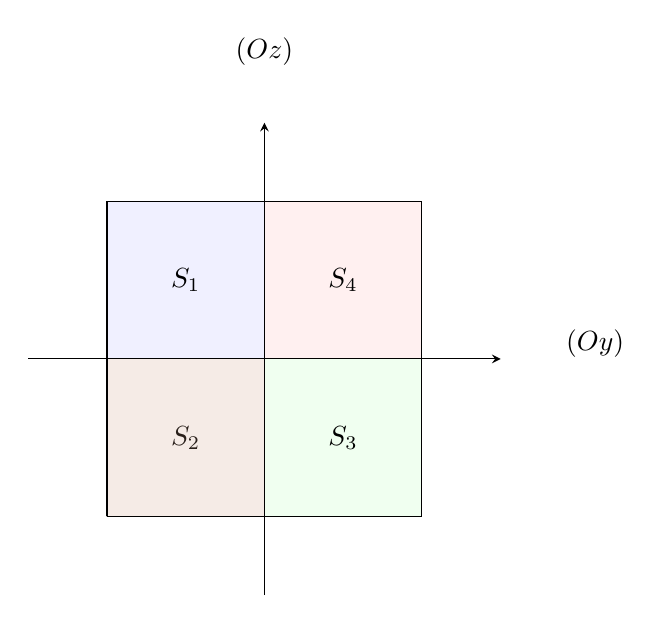
\begin{tikzpicture}[scale=2]
\filldraw[draw=black,fill=blue!30!white,opacity=0.20]
	plot (-1,0)
	-- plot (-1,1)
	-- plot (0,1)
	-- plot (0,0)
	-- cycle;	
\draw (-0.5,0.5) node{$S_1$} ;

\filldraw[draw=black,fill=red!30!white,opacity=0.20]
	plot (0,0)
	-- plot (0,1)
	-- plot (1,1)
	-- plot (1,0)
	-- cycle;	
\draw (-0.5,-0.5) node{$S_2$} ;

\filldraw[draw=black,fill=green!30!white,opacity=0.20]
	plot (0,0)
	-- plot (1,0)
	-- plot (1,-1)
	-- plot (0,-1)
	-- cycle;	
\draw (0.5,-0.5) node{$S_3$} ;

\filldraw[draw=black,fill=Sepia!30!white,opacity=0.20]
	plot (0,0)
	-- plot (0,-1)
	-- plot (-1,-1)
	-- plot (-1,0)
	-- cycle;	
\draw (0.5,0.5) node{$S_4$} ;

\draw (-1,-1) -- (1,-1) ;
\draw (-1,1) -- (1,1) ;
\draw (1,1) -- (1,-1) ;
\draw (-1,1) -- (-1,-1) ;
\draw [>=stealth, ->](-1.5,0) -- (1.5,0) ;
\draw (2.1,0.25) node[below]{$(Oy)$} ;
\draw [>=stealth, ->](0,-1.5) -- (0,1.5) ;
\draw (0,2.1) node[below]{$(Oz)$} ;
\end{tikzpicture}
\end{center}
\caption{Représentation schématique des zones $S_1$ à $S_4$ sur le panel $(I)$}
\label{fig: zones panel I}
\end{figure}

Compte tenu des symétries des harmoniques sphériques ainsi que des symétries des poids $\omega_{i,j}$, on a
\begin{equation}
\left\lbrace
\begin{array}{rcl}
S_3 & = & \bar{S}_1 \\
S_4 & = & \bar{S}_2 \\
\bar{S}_1 & = & (-1)^{m+m'+l+l'} S_1
\end{array}
\right.
\end{equation}
donc il vient :
\begin{align*}
S_{(I)} & = S_1 + S_2 + S_3 + S_4 \\
	& = S_1 + S_2 + \bar{S}_1 + \bar{S}_2 \\
	& = (1+(-1)^{l+l'+m+m'})(S_1+S_2)
\end{align*}
De plus, on a le même type de résultat pour $S_{(II)}$.

Pour le panel $(V)$, on nomme $S_a$ et $S_b$ les quantités suivantes :
\begin{align*}
S_a = & \Delta \xi \Delta \eta \gsum_{i=-N/2}^{1} \gsum_{j=-N/2}^{N/2} \omega_{i,j} (\mathbf{Y}_m^{l,*})_{i,j}^{(I)} (\bar{\mathbf{Y}}_{m'}^{l',*})_{i,j}^{(I)} \sqrt{\bar{\mathbf{G}}_{i,j}} \\
		& + \dfrac{\Delta \xi \Delta \eta}{2} \gsum_{j=-N/2}^{N/2} \omega_{0,j} (\mathbf{Y}_m^{l,*})_{0,j}^{(I)} (\bar{\mathbf{Y}}_{m'}^{l',*})_{0,j}^{(I)} \sqrt{\bar{\mathbf{G}}_{0,j}},
\end{align*}
$S_b$ est donné par la relation suivante 
\begin{align*}
S_b = & \Delta \xi \Delta \eta \gsum_{i=1}^{N/2} \gsum_{j=-N/2}^{N/2} \omega_{i,j} (\mathbf{Y}_m^{l,*})_{i,j}^{(I)} (\bar{\mathbf{Y}}_{m'}^{l',*})_{i,j}^{(I)} \sqrt{\bar{\mathbf{G}}_{i,j}} \\
		& + \dfrac{\Delta \xi \Delta \eta}{2} \gsum_{j=-N/2}^{N/2} \omega_{0,j} (\mathbf{Y}_m^{l,*})_{0,j}^{(I)} (\bar{\mathbf{Y}}_{m'}^{l',*})_{0,j}^{(I)} \sqrt{\bar{\mathbf{G}}_{0,j}}.
\end{align*}
Les zones attribuées à $S_a$ et $S_b$ sont représentées schématiquement dans la Figure \ref{fig: zones panel V}. 

\begin{figure}
\begin{center}
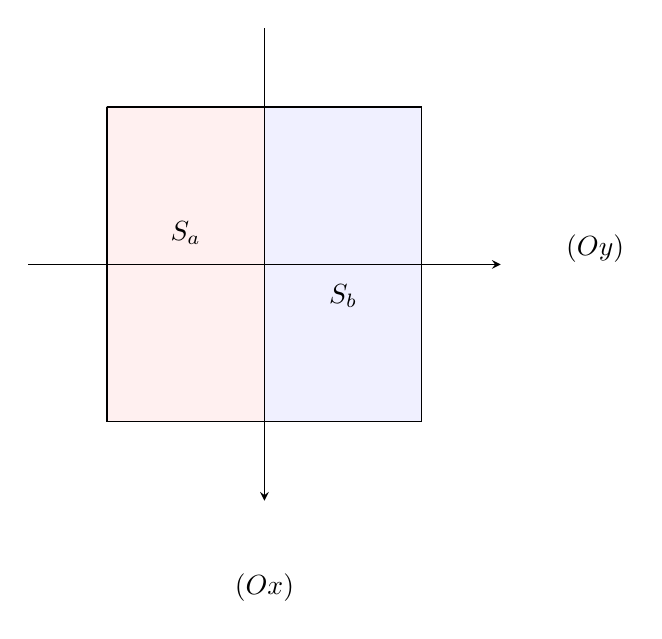
\begin{tikzpicture}[scale=2]
\filldraw[draw=black,fill=red!30!white,opacity=0.20]
	plot (-1,-1)
	-- plot (-1,1)
	-- plot (0,1)
	-- plot (0,-1)
	-- cycle;	
\filldraw[draw=black,fill=blue!30!white,opacity=0.20]
	plot (0,1)
	-- plot (1,1)
	-- plot (1,-1)
	-- plot (0,-1)
	-- cycle;	

\draw (-1,-1) -- (1,-1) ;
\draw (-1,1) -- (1,1) ;
\draw (1,1) -- (1,-1) ;
\draw (-1,1) -- (-1,-1) ;

\draw [>=stealth, ->](-1.5,0) -- (1.5,0) ;
\draw (2.1,0.25) node[below]{$(Oy)$} ;

\draw [>=stealth, ->](0,1.5) -- (0,-1.5) ;
\draw (0,-1.9) node[below]{$(Ox)$} ;

\draw (-0.5,0.2) node{$S_a$} ;
\draw (0.5,-0.2) node{$S_b$} ;

\end{tikzpicture}
\end{center}
\caption{Représentation schématique des zones $S_a$ et $S_b$ sur le panel V}
\label{fig: zones panel V}
\end{figure}
On note que :
\begin{align*}
S_{(V)} & = S_a + S_b \\
		& = S_a + (-1)^{l-l'}S_a \\
		& = (1 + (-1)^{l+l'})S_a.
\end{align*}

En faisant le bilan et en considérant les égalités démontrées, on obtient :
\begin{multline}
S = (1+(-1)^{l+l'})\left( \exp \left( -i(m+m') \dfrac{\pi}{2} \right) +1 \right)(1 +(-1)^{l+l'+m+m'})(S_1+S_2) + ...  \\
... + (1+(-1)^{l+l'+m+m'})(1 + (-1)^{l+l'})S_a.
\end{multline}
Donc $S=0$ si $m+m'$ est impair ou si $l+l'$ est impair.

Dans le cas où $m=0$ et $l=0$, on a
\begin{equation}
<\mathbf{Y}_m^{l,*},\mathbf{Y}_0^{0,*} >_{\CS} = (1+(-1)^l)\left( 1 + \exp \left( -im \dfrac{\pi}{2} \right) \right) (1 + (-1)^{l+m}) (S_1+S_2) + (1+(-1)^{l+m})(1+(-1)^l)S_a.
\end{equation}
On a déjà vu que $<\mathbf{Y}_m^{l,*},\mathbf{Y}_0^{0,*} >_{\CS} = 0$ si $l$ est impair ou $m$ impair. Dans le cas où $l \equiv 2 [4]$, on a
\begin{equation}
<\mathbf{Y}_m^{l,*},\mathbf{Y}_0^{0,*} >_{\CS} = 4 S_a.
\end{equation}
De plus $S_a = 0$ d'après le second point du lemme \ref{lem:HS_sym}. Le résultat est alors prouvé. 
\end{proof}

Dans le cas où $m+m'$ et $l+l'$ sont pairs, le produit scalaire $<\mathbf{Y}_m^l, \mathbf{Y}_{m'}^{l'}>_{\CS}$ n'est a priori pas nul. Un choix judicieux des coefficients $(\omega_{i,j})_{-N/2 \leq i,j  \leq N/2}$ permet d'assurer que cette quantité reste faible lorsque $m \neq m'$ et $l \neq l'$. C'est l'objet de la prochaine section.








































\subsection{Quadrature sur la sphère}

Les équations que nous allons résoudre sur la sphère sont des relations de conservation. De manière à étudier les propriétés de conservation du schéma utilisé, il est utile de connaître une formule de quadrature adaptée. Dans \cite{Ahrens2009, Fornberg2014}, la méthode de quadrature est conçue pour être adaptée aux harmoniques sphériques, voir aussi \cite{Mclaren1963} ou les livres \cite{Atkinson2012, Hesse2010}. Les méthodes de quadratures considérées visent à approcher l'intégrale
\begin{equation}
I(f) = \gint_{\mathbb{S}_a^2} f(\mathbf{x}) d \sigma(\mathbf{x}).
\label{eq:integrale_sphere}
\end{equation}
On note que lorsque $f = \mathbf{Y}_m^l$ est une harmonique sphérique, il s'agit d'un cas particulier de la formule \eqref{eq:HS_perp} avec $m'=l'=0$. Ainsi, on a 
\begin{equation}
I(\mathbf{Y}_m^l) = 0
\end{equation}
sauf si $m=l=0$.
Pour approcher $I(f)$, on considère des méthodes de quadrature de la forme
\begin{equation}
Q(f) = \gsum_p \omega_p f(\mathbf{x}_p)
\label{eq:quadrature_sphere}
\end{equation}
où $f : \mathbf{x} \in \mathbb{S}_a^2 \mapsto f(\mathbf{x}) \in \mathbb{C}$ est une fonction définie sur la sphère. Les points $(\mathbf{x}_p)_p$ représentent un nombre fini de points de $\mathbb{S}_a^2$, les valeurs $(\omega_p)_p$ sont des poids permettant d'approcher \eqref{eq:integrale_sphere}.

Compte tenu de la structure de la Cubed-Sphere, il est possible de construire des méthodes de quadrature par panel. On cherche des formules de quadrature proches du produit scalaire $< \cdot, \cdot >_{\CS}$ car si $f : \mathbb{S}_a^2 \mapsto \mathbb{C}$ est une fonction de $L^2(\mathbb{S}_a^2, \mathbb{C})$ alors
\begin{equation}
\gint_{\mathbb{S}_a^2} f(\mathbf{x}) d\sigma(\mathbf{x}) = <f,1>_{L^2(\mathbb{S}_a^2, \mathbb{C})}.
\end{equation}
On utilise donc des formules de quadrature de la forme
\begin{equation}
Q(\mathfrak{f}) = \gsum_{(k) = (I)}^{(VI)} Q^{(k)}(\mathfrak{f})
\end{equation}
avec $Q^{(k)}(f^*)$ une formule de quadrature par panel de la forme
\begin{equation}
Q^{(k)}(\mathfrak{f}) = \Delta \xi \Delta \eta \gsum_{i=-N/2}^{N/2} \gsum_{j=-N/2}^{N/2} \omega_{i,j} \mathfrak{f}_{i,j}^{(k)} \sqrt{\bar{\mathbf{G}}_{i,j}} \approx \gint_{(k)} f(\mathbf{x}) d \sigma(\mathbf{x})
\end{equation}
avec $\bar{\mathbf{G}}_{i,j} = \det(\mathbf{G}_{i,j})$.
Ces formules de quadratures sont étudiées dans \cite{Portelenelle2018} et donnent de très bon résultats grâce aux symétries de la Cubed-Sphere. De plus, il est possible de les améliorer en perturbant les valeurs de $(\omega_{i,j})_{-N/2 \leq i,j \leq N/2}$. Le lien avec le produit scalaire du chapitre \ref{chap:3} peut être fait directement en notant que
\begin{equation}
Q(\mathfrak{f}) = <\mathfrak{f}, \mathfrak{1}>_{\CS},
\end{equation}
où $\mathfrak{1}$ est la fonction de grille constante égale à $1$.
Or, $\mathbf{1} = a \sqrt{4 \pi} \mathbf{Y}_0^{0,*}$, donc en utilisant le théorème \ref{th:pdtscal_HS}, on obtient le corollaire suivant :
\begin{corollaire}
Toute formule de quadrature $Q$ vérifiant
\begin{equation}
\omega_{i,j} = \omega_{-i,j} = \omega_{i,-j} = \omega_{-i,-j}
\end{equation}
pour tout $-N/2 \leq i,j \leq N/2$ satisfait exactement la relation 
\begin{equation}
Q \left( \mathbf{Y}_m^{l,*} \right) = 0,
\end{equation}
avec $l \in \mathbb{N}$ et $|m| \leq l$, si
\begin{itemize}
\item $m$ est impair ou,
\item $l$ impair ou,
\item $l$ pair et $m \equiv 2 [4]$.
\end{itemize}
pour tout $N$ paramètre de la Cubed-Sphere.
\label{cor:quadrature_exacte}
\end{corollaire}

Dans la suite de ce chapitre, nous étudions différents choix de $(\omega_{i,j})_{-N/2 \leq i,j \leq N/2}$ donnant des formules de quadratures \eqref{eq:quadrature_sphere} sur la sphère $\mathbb{S}_a^2$.






















\subsection{Formules de quadrature de type trapèze}

Soient $\tf : (\xi, \eta) \in \mathbb{R}^2 \mapsto \tf(\xi, \eta) \in \mathbb{C}$ une fonction régulière et $(a,b) \in \mathbb{R}^2$ deux réels tels que $a<b$. Alors il existe un unique polynôme $P(\xi, \eta) \in \mathbb{C}[\xi, \eta]$ de degré 1 en $\xi$ et 1 en $\eta$ tel que 
\begin{equation}
\left\lbrace
\begin{array}{rcl}
P(a,a) & = & \tf(a,a) \\
P(a,b) & = & \tf(a,b) \\
P(b,a) & = & \tf(b,a) \\
P(b,b) & = & \tf(b,b).
\end{array}
\right.
\end{equation}
Ce polynôme est égal à, pour tous $(\xi, \eta) \in \mathbb{R}^2$,
\begin{equation}
P(\xi, \eta) = \dfrac{\tf(b,b)}{(a-b)^2}(\xi-a)(\eta-a) - \dfrac{\tf(a,b)}{(a-b)^2}(\xi-a)(\eta-b) -\dfrac{\tf(b,a)}{(a-b)^2}(\xi-b)(\eta-a)+ \dfrac{\tf(a,a)}{(a-b)^2}(\xi-b)(\eta-b).
\end{equation}
L'idée de la méthode des trapèzes est d'approcher l'intégrale de $\tf$ à l'aide de l'intégrale de $P$, c'est à dire
\begin{equation}
\gint_{[a,b]^2} \tf(\xi, \eta) d\xi d\eta \approx (b-a)^2 \dfrac{\tf(a,a) + \tf(a,b) + \tf(b,a) + \tf(b,b)}{4}.
\label{eq:tpzapprox}
\end{equation}
La méthode des trapèzes composite consiste à juxtaposer un ensemble de carrés pour calculer une intégrale. Plus le nombre de carrés est grand, plus l'intégrale approchée sera précise. On remarque que
\begin{equation}
\gint_{[-\pi/4,\pi/4]^2} \tf(\xi, \eta) d\xi d\eta = \gsum_{i=-N/2}^{N/2-1} \gsum_{j=-N/2}^{N/2-1} \gint_{\xi_i}^{\xi_{i+1}} \gint_{\eta_i}^{\eta_{i+1}} \tf(\xi, \eta) d\xi d\eta,
\end{equation}
avec $\xi_i = \dfrac{\pi}{4} + i \Delta \xi$ et $\eta_j = \dfrac{\pi}{4} + j \Delta \eta$. Les pas d'espace $\Delta \xi$ et $\Delta \eta$ sont
\begin{equation}
\Delta \xi = \Delta \eta = \dfrac{\pi}{2N}.
\end{equation}
On souhaite approcher l'intégrale
\begin{equation}
\gint_{[-\pi/4,\pi/4]^2} \tf(\xi, \eta) d\xi d\eta
\end{equation}
en considérant la formule \eqref{eq:tpzapprox} sur chaque carré $\left[ \xi_i, \xi_{i+1} \right] \times \left[ \eta_i, \eta_{i+1} \right]$. La formule de quadrature prend alors la forme suivante :
\begin{align*}
\gint_{[-\pi/4,\pi/4]^2} \tf(\xi, \eta) d\xi d\eta & \approx \Delta \xi \Delta \eta \gsum_{i=-N/2}^{N/2-1} \gsum_{j=-N/2}^{N/2-1} \dfrac{\tf(\xi_{i}, \eta_{j}) + \tf(\xi_{i+1}, \eta_{j}) + \tf(\xi_{i}, \eta_{j+1}) + \tf(\xi_{i+1}, \eta_{j+1}) }{4} \\
	& = \Delta \xi \Delta \eta \gsum_{i = -N/2+1}^{N/2-1} \gsum_{j = -N/2+1}^{N/2-1} \tf(\xi_i, \eta_j) + ... \\
	& \hspace{5mm} ... + \dfrac{\Delta \xi \Delta \eta}{2} \left[ \gsum_{i=-N/2+1}^{N/2-1} \left( \tf(\xi_i, \eta_{N/2} + \tf(\xi_i, \eta_{-N/2} \right) \right] + ...\\
	& \hspace{5mm} ... + \dfrac{\Delta \xi \Delta \eta}{2} \left[ \gsum_{j=-N/2+1}^{N/2-1} \left( \tf(\xi_{N/2}, \eta_{j} + \tf(\xi_{-N/2}, \eta_{j} \right) \right]+ ... \\
	& \hspace{5mm} ... + \dfrac{\Delta \xi \Delta \eta}{4} \left( \tf(\xi_{N/2}, \eta_{N/2}) + \tf(\xi_{-N/2}, \eta_{N/2}) + \tf(\xi_{N/2}, \eta_{-N/2})+ \tf(\xi_{-N/2}, \eta_{-N/2}) \right)\\
	& = \Delta \xi \Delta \eta \gsum_{i=-N/2}^{N/2} \gsum_{j=-N/2}^{N/2} \omega_{i,j} \tf(\xi_i, \eta_j).
\end{align*}
Les coefficients $(\omega_{i,j})_{-N/2 \leq i,j \leq N/2}$ sont donnés par
\begin{itemize}
\item $\omega_{-\frac{N}{2},-\frac{N}{2}}=\omega_{\frac{N}{2},-\frac{N}{2}}=\omega_{-\frac{N}{2},\frac{N}{2}}=\omega_{\frac{N}{2},\frac{N}{2}}=\frac{1}{4}$,
\item $\omega_{i,\frac{N}{2}}=\omega_{i,-\frac{N}{2}}=\frac{1}{2}$ pour $-\frac{N}{2}+1 \leq i \leq \frac{N}{2}-1$,
\item $\omega_{\frac{N}{2},j}=\omega_{-\frac{N}{2},j}=\frac{1}{2}$ pour $-\frac{N}{2}+1 \leq j \leq \frac{N}{2}-1$,
\item $\omega_{i,j}=1$ dans tous les autres cas.
\end{itemize}

Soit $f : \mathbf{x} \in \mathbb{S}_a^2 \mapsto f(\mathbf{x}) \in \mathbb{C}$ une fonction régulière. On peut appliquer la méthode des trapèzes composites à la fonction $\tf$ définie par
\begin{equation}
\tf(\xi,\eta) = f(\xi,\eta) \sqrt{\det(\mathbf{G}(\xi,\eta))} \text{ avec } -\pi/4 \leq \xi,\eta \leq \pi/4.
\end{equation}
On obtient la formule de quadrature $Q_{\tpz}$ agissant sur les fonctions de grille sur la Cubed-Sphere et définie par
\begin{equation}
Q_{\tpz}(\mathfrak{f}) = \gsum_{(k) = (I)}^{(VI)}Q_{\tpz}^{(k)}(\mathfrak{f}).
\end{equation}
Pour tout $(k) = (I), ..., (VI)$, on a
\begin{equation}
Q_{\tpz}^{(k)}(\mathfrak{f}) = \Delta \xi \Delta \eta \gsum_{i=-N/2}^{N/2} \gsum_{j=-N/2}^{N/2} \omega_{i,j} \mathfrak{f}_{i,j}^{(k)} \sqrt{\bar{\mathbf{G}}_{i,j}},
\end{equation}
où $\bar{\mathbf{G}}_{i,j}=\det(\mathbf{G}(\xi_i,\eta_j))$ pour tout $-N/2 \leq i,j \leq N/2$.

\begin{theoreme}
La formule $Q_{\tpz}$ est consistante à l'ordre 2. De plus, pour toute fonction $f : \mathbf{x} \in \mathbb{S}_a^2 \mapsto f(\mathbf{x}) \in \mathbb{C}$ régulière, on a
\begin{align*}
\gint_{(k)} f(\mathbf{x})d\sigma(\mathbf{x}) & = Q_{\tpz}^{(k)}(f^*) + ... \\
& ... + \dfrac{\Delta \xi^3}{12} \left( \gsum_{i=-N/2+1}^{N/2-1} \left( \partial_{\eta}\tf_{i, N/2} - \partial_{\eta}\tf_{i, -N/2} \right) + \gsum_{j=-N/2+1}^{N/2-1} \left( \partial_{\eta}\tf_{N/2,j} - \partial_{\eta}\tf_{-N/2,j} \right) \right) - ...  \\
	&  ... - \dfrac{\Delta \xi^3}{24} \left( \partial_{\eta}\tf_{-N/2,N/2} - \partial_{\eta}\tf_{-N/2,-N/2} + \partial_{\eta}\tf_{N/2,N/2}  - \partial_{\eta}\tf_{N/2,-N/2} \right) - ...  \\
& ... - \dfrac{\Delta \xi^3}{24} \left( \partial_{\xi}\tf_{N/2,N/2} + \partial_{\xi}\tf_{N/2,-N/2} - \partial_{\xi}\tf_{-N/2,N/2}  - \partial_{\xi}\tf_{-N/2,-N/2} \right)+...\\
& ... + \mathcal{O} \left( \Delta \xi^4 \right).
\end{align*}
en notant que $\Delta \xi = \Delta \eta$ ainsi que $\partial _{\xi} f_{i,j} = \partial_{\xi}f(\xi_i, \eta_j)$ et $\partial _{\eta} f_{i,j} = \partial_{\eta}f(\xi_i, \eta_j)$ pour tous $-N/2 \leq i,j \leq N/2$, et
\begin{equation}
\tf(\xi,\eta) = f(\xi,\eta) \sqrt{\det(\mathbf{G}(\xi,\eta))} \text{ avec } -\pi/4 \leq \xi,\eta \leq \pi/4.
\end{equation}
\label{th:quadrature_tpz}
\end{theoreme}

\begin{proof}
La fonction $\tf$ est régulière sur $[-\pi/4, \pi/4]^2$ comme produit de fonctions régulières.
La formule d'Euler MacLaurin \cite{Demailly2016, Hardy2000, Monegato1998} permet de donner une estimation de l'intégrale sur $[a,b] \subset \mathbb{R}$ :
\begin{equation}
\dfrac{1}{b-a} \gint_a^b \tf(x) dx = \dfrac{\tf(a) + \tf(b)}{2} - \gsum_{j=1}^n (b-a)^{2j-1} \dfrac{b_{2j}}{(2j)!} \left( \tf^{(2j-1)}(b) - \tf^{(2j-1)}(a)  \right) + \mathcal{O}\left( (b-a)^{2n+2}  \right) 
\end{equation}
avec $(b_{2j})$ les nombres de Bernoulli \cite{Conway2012}. En particulier on note que $b_2 = 1/6$, donc
\begin{equation}
\dfrac{1}{b-a} \gint_a^b \tf(x) dx = \dfrac{\tf(a) + \tf(b)}{2} - \dfrac{(b-a)^2}{6 \cdot 2!} \left( \tf'(a) - \tf'(b) \right) - \dfrac{(b-a)^3}{30 \cdot 4!} \left( \tf^{(3)}(a) - \tf^{(3)}(b) \right) + \mathcal{O}\left( (b-a)^4 \right). 
\end{equation}
Ainsi, la formule suivante est vérifiée :
\begin{align*}
\gint_{-\pi/4}^{\pi/4} \tf(\xi, \eta) d\xi & = \gsum_{i=-N/2}^{N/2-1} \gint_{\xi_i}^{\xi_{i+1}} \tf(\xi, \eta) d\xi \\
	& = \dfrac{\Delta \xi}{2} \tf(\xi_{-N/2}, \eta) + \Delta \xi \gsum_{-N/2+1}^{N/2-1} \tf(\xi_i, \eta) + \dfrac{\Delta \xi}{2} \tf(\xi_{N/2}, \eta) - ... \\
	& \hspace{1cm}... - \dfrac{\Delta \xi^3}{24} \left( \gsum_{i=-N/2+1}^{N/2-1} \left( \partial_{\eta}\tf_{i, N/2} - \partial_{\eta}\tf_{i, -N/2} \right) + \gsum_{j=-N/2+1}^{N/2-1} \left( \partial_{\eta}\tf_{N/2,j} - \partial_{\eta}\tf_{-N/2,j} \right) \right) - ...  \\
	& \hspace{1cm} ... - \dfrac{\Delta \xi^2}{12} \left(\partial_{\xi} \tf(\xi_{N/2},\eta)- \partial_{\xi} \tf(\xi_{-N/2},\eta)  \right) + ...\\
	& \hspace{1cm} ... - \dfrac{\Delta \xi^3}{720} \left(\partial_{\xi}^{(3)} \tf(\xi_{N/2},\eta)- \partial_{\xi}^{(3)}\tf(\xi_{-N/2},\eta)  \right) + \mathcal{O} \left( \Delta \xi^4 \right).
\end{align*}
On intègre cette dernière relation par rapport à $\eta \in [- \pi/4, \pi/4]$ et en utilisant à nouveau la formule d'Euler-MacLaurin, on obtient
\begin{align*}
\gint_{(k)} f(\mathbf{x})d\sigma(\mathbf{x}) & = Q_{\tpz}^{(k)}(f^*) + ... \\
& ... + \dfrac{\Delta \xi^3}{12} \left( \gsum_{i=-N/2+1}^{N/2-1} \left( \partial_{\eta}\tf_{i, N/2} - \partial_{\eta}\tf_{i, -N/2} \right) + \gsum_{j=-N/2+1}^{N/2-1} \left( \partial_{\eta}\tf_{N/2,j} - \partial_{\eta}\tf_{-N/2,j} \right) \right) - ...  \\
	&  ... - \dfrac{\Delta \xi^3}{24} \left( \partial_{\eta}\tf_{-N/2,N/2} - \partial_{\eta}\tf_{-N/2,-N/2} + \partial_{\eta}\tf_{N/2,N/2}  - \partial_{\eta}\tf_{N/2,-N/2} \right) - ...  \\
& ... - \dfrac{\Delta \xi^3}{24} \left( \partial_{\xi}\tf_{N/2,N/2} + \partial_{\xi}\tf_{N/2,-N/2} - \partial_{\xi}\tf_{-N/2,N/2}  - \partial_{\xi}\tf_{-N/2,-N/2} \right)+...\\
& ... + \mathcal{O} \left( \Delta \xi^4 \right).
\end{align*}
Cette dernière relation permet d'obtenir
\begin{equation}
Q_{\tpz}(f^*) - \gint_{(k)} f(\mathbf{x})d\sigma(\mathbf{x}) = \mathcal{O}(\Delta \xi^2).
\end{equation}
Alors par somme sur $(k)$, on montre que la formule $Q_{\tpz}$ est consistante avec l'intégrale à l'ordre 2.
\end{proof}


\begin{remarque}
On note que si $-N/2 \leq i,j \leq N/2$ alors on a 
\begin{equation}
\omega_{i,j} = \omega_{-i,j} = \omega_{i,-j} = \omega_{-i,-j} > 0
\end{equation}
donc le corollaire \ref{cor:quadrature_exacte} est vérifié pour la formule de quadrature $Q_{\tpz}$.
\end{remarque}



























\subsection{Formule de quadrature de type Simpson}

Dans cette section, on considère $N$ pair.
La formule de quadrature de Simpson est basée sur une approximation polynomiale de $\tf$ en trois points. L'approximation de Simpson s'exprime sous la forme :
\begin{equation}
\gint_a^b \tf(\xi, \eta) d\xi \approx \dfrac{b-a}{6} \left( \tf(a,\eta) + 4  \tf \left( \dfrac{a+b}{2},\eta \right) + \tf(b,\eta) \right) 
\end{equation}
Il s'agit d'une approximation plus précise que la méthode des trapèzes. En effet si $g : x \in [a,b] \mapsto g(x) \in \mathbb{C}$ alors
\begin{equation}
\gint_a^b g(x)dx - \dfrac{b-a}{6} \left( g(a) + 4 g\left( \dfrac{a+b}{2} \right) + g(b) \right) = \mathcal{O}((b-a)^5).
\end{equation}
Il s'agit d'une méthode classique d'approximation d'intégrale \cite{Hammerlin1991}.

Ainsi, la formule de Simpson composite s'obtient en juxtaposant des intervalles de la forme $\left[ \xi_{i-1}, \xi_{i+1} \right]$ pour calculer l'intégrale sur $\left[ -\dfrac{\pi}{4} , \dfrac{\pi}{4} \right]$ :
\begin{equation}
\gint_{- \pi/4}^{\pi/4} \tf(\xi, \eta) d\xi = \gsum_{i=-N/2, \text{pair}}^{N/2} \gint_{\xi_{i-1}}^{\xi_{i+1}} \tf(\xi, \eta) d\xi.
\end{equation}
En considérant l'approximation de Simpson sur chaque intervalle $\left[ \xi_{i-1}, \xi_{i+1} \right]$, on obtient
\begin{equation}
\gint_{-\pi/4}^{\pi/4} \tf(\xi, \eta) d\xi = \dfrac{\Delta \xi}{3} \left[ \tf(\xi_{-N/2}, \eta) + 2 \gsum_{i=-N/4-1}^{N/4} \tf(\xi_{2i}, \eta)  + 4 \gsum_{i=-N/4}^{N/4} \tf(\xi_{2i-1}, \eta) + \tf(\xi_{N/2}, \eta) \right] + \mathcal{O}\left( \Delta \xi^4\right).
\end{equation}
On intègre cette équation par rapport à $\eta$ et on utilise la même approximation dans la direction $\eta$ :
\begin{equation}
\gint_{-\frac{\pi}{4}}^{\frac{\pi}{4}} \gint_{-\frac{\pi}{4}}^{\frac{\pi}{4}} \tf(\xi, \eta) d\xi  d\eta= \Delta\xi \Delta \eta \gsum_{i=-N/2}^{N/2}\gsum_{j=-N/2}^{N/2} \omega_{i,j} \tf(\xi_i, \eta_j) + \mathcal{O}\left( \Delta \xi^4\right)
\label{eq:simpson 2d}
\end{equation}
où les coefficients $(\omega_{i,j})_{-N/2 \leq i,j \leq N/2}$ sont donnés par
\begin{itemize}
\item $\omega_{\frac{N}{2},\frac{N}{2}}=\omega_{\frac{N}{2},-\frac{N}{2}}=\omega_{-\frac{N}{2},\frac{N}{2}}=\omega_{-\frac{N}{2},-\frac{N}{2}}=1/9$,
\item $\omega_{\frac{N}{2},i}=\omega_{-\frac{N}{2},i}=\omega_{i,\frac{N}{2}}=\omega_{i,-\frac{N}{2}}=4/9$ si $i$ est pair,
\item $\omega_{\frac{N}{2},i}=\omega_{-\frac{N}{2},i}=\omega_{i,\frac{N}{2}}=\omega_{i,-\frac{N}{2}}=2/9$ si $i$ est impair,
\item $\omega_{i,j}=16/9$ si $i$ et $j$ sont pairs,
\item $\omega_{i,j}=4/9$ si $i$ et $j$ sont impairs,
\item $\omega_{i,j}=8/9$ dans les autres cas.
\end{itemize}

On déduit la formule de quadrature sur la sphère. Soit $\tf$ la fonction défini par
\begin{equation}
\tf(\xi, \eta) = f(\xi, \eta) \sqrt{\det(\mathbf{G}(\xi, \eta)}.
\end{equation}
On trouve la formule de quadrature de type Simpson,
pour tout $(k) = (I), ..., (VI)$, on a
\begin{equation}
Q_{\sps}^{(k)}(\mathfrak{f}) = \Delta \xi \Delta \eta \gsum_{i=-N/2}^{N/2} \gsum_{j=-N/2}^{N/2} \omega_{i,j} \mathfrak{f}_{i,j}^{(k)} \sqrt{\bar{\mathbf{G}}_{i,j}},
\end{equation}
où $\bar{\mathbf{G}}_{i,j}=\det(\mathbf{G}(\xi_i,\eta_j))$ pour tout $-N/2 \leq i,j \leq N/2$. On note aussi la formule de quadrature
\begin{equation}
Q_{\sps}(\mathfrak{f}) = \gsum_{(k)=(I)}^{(VI)}Q_{\sps}^{(k)}(\mathfrak{f}).
\end{equation}
La formule $Q_{\sps}$ est consistante à l'ordre 4 au sens du théorème suivant :


\begin{theoreme}
Soit $f : \mathbf{x} \in \mathbb{S}_a^2 \mapsto f(\mathbf{x}) \in \mathbb{C}$ une fonction régulière, alors
\begin{equation}
\gint_{\mathbb{S}_a^2} f(\mathbf{x}) d\sigma(\mathbf{x}) - Q_{\sps}(f^*) = \mathcal{O} \left( \Delta \xi^4 \right),
\end{equation}
ainsi que pour $(k) = (I), ..., (VI)$
\begin{equation}
\gint_{(k)} f(\mathbf{x}) d\sigma(\mathbf{x}) - Q_{\sps}^{(k)}(f^*) = \mathcal{O} \left( \Delta \xi^4 \right),
\end{equation}
lorsque $N$ est pair.
\end{theoreme}

\begin{remarque}
Comme pour la formule de quadrature $Q_{\tpz}$, si $-N/2 \leq i,j \leq N/2$ alors on a 
\begin{equation}
\omega_{i,j} = \omega_{-i,j} = \omega_{i,-j} = \omega_{-i,-j} > 0
\end{equation}
donc le corollaire \ref{cor:quadrature_exacte} est vérifié pour la formule de quadrature $Q_{\sps}$.
\end{remarque}





















\subsection{Formule de quadrature de type $Q_{\alpha}$}

La formule de quadrature $Q_{\tpz}$ est précise à l'ordre 2. De plus, elle ne dépend pas de la parité de $N$ le paramètre de la Cubed-Sphere. Dans cette partie, nous considérons la formule de quadrature $Q_{\alpha}$ basée sur une perturbation de $Q_{\tpz}$.
\begin{definition}
On définit $Q_{\alpha}$ la formule de quadrature agissant sur les fonctions de grilles sur la Cubed-Sphere $\mathfrak{f}$ par
\begin{equation}
Q_{\alpha}(\mathfrak{f})= \gsum_{(k)=(I)}^{(VI)} Q^{(k)}_{\alpha}(\mathfrak{f})
\end{equation}
où $Q^{(k)}_{\alpha}$ est la règle de quadrature par panel donnée par
\begin{equation}
Q_{\alpha}^{(k)}(\mathfrak{f})=\gsum_{i = -\frac{N}{2}}^{\frac{N}{2}}\gsum_{j = -\frac{N}{2}}^{\frac{N}{2}} \Delta \xi \Delta \eta \omega_{i,j} \mathfrak{f}_{i,j}^{(k)} \sqrt{\mathbf{\bar{G}}^{(k)}(\xi_i, \eta_j)}.
\label{eq:alpha par panel}
\end{equation}
Les coefficients $(\omega_{i,j})_{-N/2 \leq i,j \leq N/2}$ vérifient :
\begin{itemize}
\item $\omega_{-\frac{N}{2},-\frac{N}{2}}=\omega_{\frac{N}{2},-\frac{N}{2}}=\omega_{-\frac{N}{2},\frac{N}{2}}=\omega_{\frac{N}{2},\frac{N}{2}}=\alpha$,
\item $\omega_{i,\frac{N}{2}}=\omega_{i,-\frac{N}{2}}=\frac{1}{2}$ pour $-\frac{N}{2}+1 \leq i \leq \frac{N}{2}-1$,
\item $\omega_{\frac{N}{2},j}=\omega_{-\frac{N}{2},j}=\frac{1}{2}$ pour $-\frac{N}{2}+1 \leq j \leq \frac{N}{2}-1$,
\item $\omega_{i,j}=1$ dans tous les autres cas.
\end{itemize}
\end{definition} 

Le paramètre $\alpha$ est un paramètre qui permettra d'optimiser cette formule de quadrature.
En particulier, on a
\begin{equation}
Q_{\tpz} = Q_{1/4}.
\end{equation}

La formule ainsi perturbée permet de retrouver des résultats de précision semblables à ceux que $Q_{\tpz}$. En effet, on a la proposition suivante :
\begin{proposition}
Soit $f: \mathbf{x} \in \mathbb{S}_a^2 \rightarrow f(\mathbf{x}) \in \mathbb{C}$ une fonction régulière alors :
\begin{equation}
I^{(k)}(f) - Q^{(k)}_{\alpha}(f^*) = \mathcal{O} \left( \Delta \xi^2 \right)
\end{equation}
pour tout $(k) \in \lbrace (I), ..., (VI) \rbrace$.
De plus, on a
\begin{equation}
I(f) - Q_{\alpha}(f^*) = \mathcal{O}(\Delta \xi^2).
\end{equation}
\label{prop:consistance alpha panel}
\end{proposition}

\begin{proof}
La fonction $f$ est régulière, donc on a
\begin{align*}
I^{(k)}(f) - Q^{(k)}_{\alpha}(f^*) & = I^{(k)}(f) - Q^{(k)}_{\tpz}(f^*) + Q^{(k)}_{\tpz}(f^*) - Q^{(k)}_{\alpha}(f^*)\\
	& =  Q^{(k)}_{\tpz}(f^*) - Q^{(k)}_{\alpha}(f^*) + \mathcal{O}(\Delta \xi^2) \\
	& = 3\Delta \xi \Delta \eta \left( \dfrac{1}{4} - \alpha \right) \gsum_{(\xi, \eta) \in C} f(\xi, \eta) \sqrt{\det(\mathbf{G}(\xi, \eta))}  + \mathcal{O}(\Delta \xi^2)
\end{align*}
où $C$ désigne l'ensemble des coins de la Cubed-Sphere.

De plus $(\xi, \eta) \in [-\pi/4, \pi/4]^2 \mapsto f(\xi, \eta) \sqrt{\det(\mathbf{G}(\xi, \eta))}$ est continue sur un compact donc bornée. Ainsi
\begin{equation}
I^{(k)}(f) - Q^{(k)}_{\alpha}(f^*) = \mathcal{O}(\Delta \xi^2).
\end{equation}
En sommant cette formule sur chaque panel, on montre la consistance de $Q_{\alpha}$ avec l'intégrale sur la sphère $\mathbb{S}_a^2$.
\end{proof}

\begin{proposition}
La méthode $Q_{\alpha}$ est d'ordre 2.
\end{proposition}

\begin{proof}
La preuve de ce résultat consiste à montrer que la formule $Q_{\alpha}$ est d'ordre 2 mais pas d'ordre supérieur.
On pose
\begin{equation}
\bar{\mathbf{G}}(\mathbf{x}) = \det (\mathbf{G}(\mathbf{x})).
\end{equation}
On choisit $f$ tel que pour tout $\mathbf{x} \in \mathbb{S}_a^2$, on ait $f(\mathbf{x})=\dfrac{1}{\sqrt{\overline{\mathbf{G}}(\mathbf{x})}}$. Alors on sait que l’égalité suivante est exactement vérifiée pour tout $N$ paramètre de maillage de la Sphère.
\begin{equation}
Q_{\tpz}(f^*)-I(f)=0
\end{equation}
De plus pour tout $(\xi,\eta) \in C=\{(\pi/4,\pi/4),(-\pi/4,\pi/4),(\pi/4,-\pi/4),(-\pi/4,-\pi/4) \}$, on a :
\begin{equation}
f(\xi,\eta)\sqrt{\overline{\mathbf{G}}(\xi,\eta}=1
\end{equation}
d'où :
\begin{align*}
Q_{\alpha}(f^*)-Q_{\tpz}(f) & = 3 \Delta \xi \Delta \eta \left( \alpha - \dfrac{1}{4} \right)\gsum_{(\xi,\eta)\in C} f(\xi,\eta)\sqrt{\overline{\mathbf{G}}(\xi,\eta)} \\
                         & = 24 \Delta \xi \Delta \eta \left( \alpha - \dfrac{1}{4} \right),
\end{align*}
donc :
\begin{align*}
Q_{\alpha}(f^*) - I(f) & = Q_{\alpha}(f^*) - Q_{\tpz}(f^*) + Q_{\tpz}(f^*) - I(f) \\
                    & = 24 \Delta \xi \Delta \eta \left( \alpha - \dfrac{1}{4} \right) + \mathcal{O} \left( \Delta \xi^2 \right)
\end{align*}
La méthode de quadrature $Q_{\alpha}$ ne peut donc pas être d'un ordre supérieur à 2. 
\end{proof}



\begin{proposition}
Soit $(k) = (I), \cdots , (VI)$ un panel fixé.
Le coefficient $\alpha=1/3$ optimise la quantité
\begin{equation}
|Q_{\alpha}^{(k)}(\mathbf{1}) - I^{(k)}(\mathbf{1}) |
\end{equation}
au sens où
\begin{equation}
|Q_{1/3}^{(k)}(\mathbf{1}) - I^{(k)}(\mathbf{1}) | = \mathcal{O}\left( \Delta \xi^4 \right).
\end{equation}
\end{proposition}

\begin{proof}
On pose $f = \sqrt{\det(\mathbf{G})}$, alors par comparaison avec la méthode des trapèzes, on a 
\begin{align*}
Q_{\alpha}^{(k)}(\mathbf{1}) - I^{(k)}(\mathbf{1}) & = Q_{\alpha}(\mathbf{1}) - Q_{\tpz}(\mathbf{1}) + Q_{\tpz}(\mathbf{1}) - I^{(k)}(\mathbf{1})\\
	& = \Delta \xi^2 \left( \alpha - \dfrac{1}{4} \right) \left( f_{N/2,N/2} + f_{-N/2,N/2}+ f_{N/2,-N/2}+ f_{-N/2,-N/2} \right) + ...\\
	& \hspace{.6cm} ... + \dfrac{\Delta \xi^3}{12} \left( \gsum_{i=-N/2+1}^{N/2-1} \left( \partial_{\eta}\tf_{i, N/2} - \partial_{\eta}\tf_{i, -N/2} \right) + \gsum_{j=-N/2+1}^{N/2-1} \left( \partial_{\eta}\tf_{N/2,j} - \partial_{\eta}\tf_{-N/2,j} \right) \right) - ...  \\
	&  \hspace{.6cm}... - \dfrac{\Delta \xi^3}{24} \left( \partial_{\eta}\tf_{-N/2,N/2} - \partial_{\eta}\tf_{-N/2,-N/2} + \partial_{\eta}\tf_{N/2,N/2}  - \partial_{\eta}\tf_{N/2,-N/2} \right) - ...  \\
& \hspace{.6cm}... - \dfrac{\Delta \xi^3}{24} \left( \partial_{\xi}\tf_{N/2,N/2} + \partial_{\xi}\tf_{N/2,-N/2} - \partial_{\xi}\tf_{-N/2,N/2}  - \partial_{\xi}\tf_{-N/2,-N/2} \right)+...\\
& \hspace{.6cm}... + \mathcal{O} \left( \Delta \xi^4. \right).
\end{align*}
On note en particulier que 
\begin{equation}
f_{N/2,N/2} = f_{-N/2,N/2} = f_{N/2,-N/2} = f_{-N/2,-N/2} = \sqrt{\bar{\mathbf{G}}(\pi/4,\pi/4)} = \dfrac{4a^2}{3 \sqrt{3}} 
\end{equation}
en posant $\bar{\mathbf{G}} = \det (\mathbf{G})$.

De plus, en dérivant $\sqrt{\bar{\mathbf{G}}} = a^2 \dfrac{(1+X^2)(1+Y^2)}{(1+X^2+Y^2)^{3/2}}$ avec $X=\tan (\xi)$ et $Y=\tan (\eta)$ on obtient les relations suivantes :
\begin{equation}
\partial_{\xi} f = X \left(\dfrac{3Y^2}{1+X^2+Y^2}-1\right) \sqrt{\bar{\mathbf{G}}}
\end{equation}
\begin{equation}
\partial_{\eta} f = Y \left(\dfrac{3X^2}{1+X^2+Y^2}-1\right) \sqrt{\bar{\mathbf{G}}}.
\end{equation}
Ainsi :
\begin{itemize}
\item $\partial_{\xi} f_{N/2,j} = -\partial_{\xi} f_{-N/2,j} = 4 \dfrac{Y^4-1}{(Y^2+2)^{5/2}} a^2$,
\item $\partial_{\eta} f_{i,N/2} = -\partial_{\eta} f_{i,-N/2} = 4 \dfrac{X^4-1}{(X^2+2)^{5/2}} a^2$.
\end{itemize}
d'où le terme d'ordre 2 est
\begin{equation}
\Delta \xi^2 a^2 \left( \alpha - \dfrac{1}{4} \right) \dfrac{16}{3 \sqrt{3}} + \dfrac{4}{3}S
\label{eq:optimalite alpha 2}
\end{equation}
avec $S=\Delta \xi \gsum_{i=-N/2+1}^{N/2-1} g(i \Delta \xi)$ avec $g$ la fonction $g:x \mapsto g(x)=\dfrac{\tan(x)^4 -1}{(\tan(x)^2+2)^{5/2}}$.

Comme $g\left(-\frac{\pi}{4} \right)=g\left(\frac{\pi}{4} \right)=0$ et par propriété de la formule des trapèzes, on note que :
\begin{equation}
S = \dfrac{g\left(-\frac{\pi}{4} \right)+g\left(\frac{\pi}{4} \right)}{2} + \gint_{-\pi/4}^{\pi/4} g(x)dx + \mathcal{O}\left( \Delta \xi^2 \right) = -\dfrac{1}{3\sqrt{3}} + \mathcal{O}\left( \Delta \xi^2 \right).
\end{equation}
Donc le terme d'ordre 2 s’annule à condition que :
\begin{equation}
\left(\alpha - \dfrac{1}{4} \right) \dfrac{16}{3 \sqrt{3}} - \dfrac{4}{9 \sqrt{3}} = 0.
\end{equation}
Cette condition est vérifiée pour $\alpha = 1/3$.

Le terme d'ordre 3 s'écrit
\begin{multline}
- \dfrac{\Delta \xi^3}{24} \left[ \partial_{\eta} f_{-\frac{N}{2},\frac{N}{2}} - \partial_{\eta} f_{-\frac{N}{2},-\frac{N}{2}} + \partial_{\eta} f_{\frac{N}{2},\frac{N}{2}} -\partial_{\eta} f_{\frac{N}{2},-\frac{N}{2}}  \right] \\
-\dfrac{\Delta \xi^3}{24} \left[ \partial_{\xi} f_{\frac{N}{2},\frac{N}{2}} + \partial_{\xi} f_{\frac{N}{2},-\frac{N}{2}} - \partial_{\xi} f_{-\frac{N}{2},\frac{N}{2}} -\partial_{\xi} f_{-\frac{N}{2},-\frac{N}{2}}  \right]
\label{eq:opimalite alpha 3}
\end{multline}
on note que :
\begin{equation}
\partial_{\eta} f_{\frac{N}{2},\frac{N}{2}} = \partial_{\eta} f_{-\frac{N}{2},\frac{N}{2}} = \partial_{\eta} f_{\frac{N}{2},-\frac{N}{2}} = \partial_{\eta} f_{-\frac{N}{2},-\frac{N}{2}} = 0.
\end{equation}
De la même manière, en $\xi$ :
\begin{equation}
\partial_{\xi} f_{\frac{N}{2},\frac{N}{2}} = \partial_{\xi} f_{-\frac{N}{2},\frac{N}{2}} = \partial_{\xi} f_{\frac{N}{2},-\frac{N}{2}} = \partial_{\xi} f_{-\frac{N}{2},-\frac{N}{2}} = 0 
\end{equation}
d'où le résultat :
\begin{equation}
|Q_{1/3}^{(k)}(\mathbf{1}) - I^{(k)}(\mathbf{1}) | = \mathcal{O}\left( \Delta \xi^4 \right)
\end{equation}
\end{proof}

\begin{remarque}
Ce résultat d'optimalité s'écrit également sur la sphère $\mathbb{S}_a^2$ :
\begin{equation}
|Q_{1/3}(\mathbf{1}) - I(\mathbf{1}) | = \mathcal{O}\left( \Delta \xi^4 \right).
\end{equation}
\end{remarque}

\begin{remarque}
La formule de quadrature $Q_{\alpha}$ vérifie le corollaire \ref{cor:quadrature_exacte}.
\end{remarque}





















\subsection{Résultats numériques pour les formules de quadratures}

Pour tester numériquement les performances des formules de quadrature introduites dans les sections précédentes, on s’intéresse à un ensemble de fonctions sur la sphère dont l'intégrale est connue. Ces fonctions sont utilisées pour tester la précision des formules de quadrature sphériques \cite{Fornberg2014}. Elles sont données pour $(x,y,z) \in \mathbb{S}_a^2$ par
\begin{itemize}
\item $f_0(x,y,z)=1$,
\begin{equation}
\gint_{\mathbb{S}_a^2} f_0(\mathbf{x}) d\sigma (\mathbf{x})=4 \pi a^2,
\end{equation}
\item $f_1(x,y,z)=1+x+y^2+y\cdot x^2+x^4+y^5+x^2 \cdot y^2 \cdot z^2$,
\begin{equation}
\gint_{\mathbb{S}_a^2} f_1(\mathbf{x}) d\sigma (\mathbf{x})=\dfrac{216 \pi}{35} a^2,
\end{equation}
\item la fonction $f_2$ vérifie 
\begin{equation}
\begin{array}{rcl}
f_2(x,y,z) & = & \dfrac{3}{4} \exp \left[ - \dfrac{(9x-2)^2}{4} - \dfrac{(9y-2)^2}{4} - \dfrac{(9z-2)^2}{4} \right] + ...\\
& & ... + \dfrac{3}{4} \exp \left[ - \dfrac{(9x+1)^2}{49} - \dfrac{9y+1}{10} - \dfrac{9z+1}{10} \right] + ...\\
& & ... + \dfrac{1}{2} \exp \left[ - \dfrac{(9x-7)^2}{4} - \dfrac{(9y-3)^3}{4} - \dfrac{(9z-5)^2}{4} \right] + ...\\
& &... + \dfrac{1}{5} \exp \left[ - (9x-4)^2 - (9y-7)^2 - (9z-5)^2 \right]
\end{array}
\end{equation}
et s'intègre :
\begin{equation}
\gint_{\mathbb{S}_a^2} f_2(\mathbf{x}) d\sigma (\mathbf{x})=a^2 \cdot 6.6961822200736179523...
\end{equation}
\item $f_3(x,y,z)=\frac{1+\tanh(-9x-9y+9z)}{9}$,
\begin{equation}
\gint_{\mathbb{S}_a^2} f_3(\mathbf{x}) d\sigma (\mathbf{x})=\frac{4\pi}{9} a^2,
\end{equation}
\item $f_4(x,y,z)=\frac{1+\sign(-9x-9y+9z)}{9}$,
\begin{equation}
\gint_{\mathbb{S}_a^2} f_4(\mathbf{x}) d\sigma (\mathbf{x})=\frac{4\pi}{9} a^2,
\end{equation}
\item $f_5(x,y,z)=\frac{1-\sign(\pi x + y)}{\nu}$,
\begin{equation}
\gint_{\mathbb{S}_a^2} f_5(\mathbf{x}) d\sigma (\mathbf{x})=\frac{4\pi}{\nu} a^2.
\end{equation}
Dans les tests effectués, nous choisissons $\nu = 7$.
\end{itemize}

On note en particulier que la fonction $f_1$ est polynomiale donc régulière et elle ne fait intervenir qu'un nombre fini d'harmoniques sphériques dans sa décomposition. Les fonctions $f_2$ et $f_3$ font intervenir un plus grand nombre d'harmoniques sphériques et sont régulières.
Les fonctions $f_4$ et $f_5$ sont discontinues. 

Pour chacune de ces fonctions, on mesure l'erreur relative donnée par
\begin{equation}
e_r(f) = \dfrac{|I(f) - Q(f^*)|}{|I(f)|}
\end{equation}
où $I(f)$ représente l'intégrale exacte sur la sphère $\mathbb{S}_a^2$, $Q(f^*)$ est la valeur approchée obtenue par une formule de quadrature.
Nous retenons l'erreur maximale obtenue après $1000$ rotations aléatoires de $f$.

Cette erreur est mesurée pour différentes grilles Cubed-Sphere de taille $N \times N \times 6$ avec $N=8$, $N=16$, $N=32$, $N=64$, $N=128$ et $N=256$. On peut ainsi mesurer l'ordre de convergence. Les résultats sont donnés dans la figure \ref{fig:rate_quad}.


\begin{figure}[htbp]
\begin{center}
\includegraphics[width=8cm]{quadf0.jpg}
\includegraphics[width=8cm]{quadf1.jpg}\\
\includegraphics[width=8cm]{quadf2.jpg}
\includegraphics[width=8cm]{quadf3.jpg}\\
\includegraphics[width=8cm]{quadf4.jpg}
\includegraphics[width=8cm]{quadf5.jpg}\\
\end{center}
\caption{Taux de convergence pour différentes méthodes de quadratures pour les fonctions tests $(f_p)_{0 \leq p \leq 5}$. Nous retenons l'erreur maximale après $1000$ rotations aléatoires pour chaque grille Cubed-Sphere de paramètre $N=8$, $N=16$, $N=32$, $N=64$, $N=128$ et $N=256$. De haut en bas et de gauche à droite, les fonctions sont $f_0$, $f_1$, $f_2$, $f_3$, $f_4$ et $f_5$. Le taux de convergence est proche de $4$ pour $Q_{\sps}$ et $Q_{1/3}$, il est proche de $2$ pour $Q_{\tpz}$ et $Q_1$.}
\label{fig:rate_quad}
\end{figure}

Les taux de convergence observées sont ceux attendus. Pour $Q_{\tpz}$ et $Q_{\alpha}$ avec $\alpha=1$, le taux de convergence est proche de $2$. Pour la formule de quadrature $Q_{\sps}$, l'ordre de convergence est proche de $4$. La formule de quadrature $Q_{\alpha}$ avec $\alpha = 1/3$ présente de meilleurs résultats que ceux attendus. On observe que la méthode est d'ordre $4$ pour tous les tests effectués.

Nous avons étudié ici différents type de formules de quadrature sur la grille Cubed-Sphere qui sera utilisée pour la résolution des équations. Toutes les formules étudiées définissent un produit scalaire possédant de bonnes propriétés d'orthogonalité des harmoniques sphériques.

La formule $Q_{\tpz}$ est basée sur la formule des trapèzes composites, cette formule est consistante avec l'intégrale à l'ordre 2. La formule $Q_{\sps}$ est conçue à partir de la méthode de Simpson, elle est consistante à l'ordre 4 lorsque $N$ est pair. Cette propriété de précision est fausse lorsque $N$ est impair.
Les formules de quadrature $Q_{\alpha}$ sont des perturbations de la formule $Q_{\tpz}$. Le paramètre $\alpha>0$ permet de pondérer les coins de la Cubed-Sphere. Quel que soit le choix de $\alpha$, la formule $Q_{\alpha}$ est consistante avec l'intégrale au moins à l'ordre 2. Lorsque $\alpha = 1/3$, on prouve que la méthode est plus précise pour intégrer les fonctions constantes.

Lors des tests numériques, nous avons pu vérifier les ordres de convergence théoriques. De plus, la formule $Q_{1/3}$ semble particulièrement efficace puisqu'une convergence à l'ordre 4 est observée.

Dans la suite de ce travail, nous retenons la formule de quadrature $Q_{\alpha}$ avec $\alpha = 1/3$ pour étudier les propriétés de conservation des schémas numériques utilisés.







\textcolor{white}{
\begin{flushright}
\textit{"En mathématiques, on ne comprend pas les choses, on s'y habitue." },
John Von Neumann.
\end{flushright}
}










